\documentclass[12pt,a4paper]{report}

% -----------------------------------------------------------------------------
% Graphic Era Hill University - Project Report Format Specifications
% Annexure I: Margins: Left 3.5cm, Top 2.5cm, Right 1.25cm, Bottom 1.25cm
% 1.5 Line Spacing, Times New Roman Font
% -----------------------------------------------------------------------------
\usepackage[left=3.5cm, top=2.5cm, right=1.25cm, bottom=1.25cm]{geometry}
\usepackage{setspace}
\onehalfspacing

\usepackage{mathptmx} % Times New Roman font
\usepackage{graphicx}
\usepackage{amsmath,amssymb}
\usepackage{booktabs}
\usepackage{tabularx}
\usepackage{longtable}
\usepackage{multirow}
\usepackage{listings}
\usepackage{xcolor}
\usepackage{hyperref}
\usepackage{fancyhdr}
\usepackage{titlesec}
\usepackage{caption}
\usepackage{subcaption}

% Code Listing Styling
\definecolor{codegreen}{rgb}{0,0.6,0}
\definecolor{codegray}{rgb}{0.5,0.5,0.5}
\definecolor{codepurple}{rgb}{0.58,0,0.82}
\definecolor{backcolour}{rgb}{0.97,0.97,0.97}

\lstdefinestyle{mystyle}{
    backgroundcolor=\color{backcolour},   
    commentstyle=\color{codegreen},
    keywordstyle=\color{magenta},
    numberstyle=\tiny\color{codegray},
    stringstyle=\color{codepurple},
    basicstyle=\ttfamily\footnotesize,
    breakatwhitespace=false,         
    breaklines=true,                 
    captionpos=b,                    
    keepspaces=true,                 
    numbers=left,                    
    numbersep=5pt,                  
    showspaces=false,                
    showstringspaces=false,
    showtabs=false,                  
    tabsize=2
}
\lstset{style=mystyle}

\hypersetup{
    colorlinks=true,
    linkcolor=black,
    citecolor=black,
    filecolor=black,
    urlcolor=blue
}

% Page numbering and headers
\pagestyle{fancy}
\fancyhf{}
\fancyhead[R]{\thepage}
\renewcommand{\headrulewidth}{0.4pt}
\fancypagestyle{plain}{
  \fancyhf{}
  \fancyhead[R]{\thepage}
  \renewcommand{\headrulewidth}{0pt}
}

\begin{document}

% =============================================================================
% ANNEXURE II: COVER PAGE
% =============================================================================
\begin{titlepage}
\begin{center}
    \vspace*{0.2cm}
    {\fontsize{16pt}{20pt}\selectfont \textbf{STAYMART: SMART STUDENT HOUSING AND CAMPUS MARKETPLACE}\par}
    
    \vspace{1.0cm}
    {\fontsize{12pt}{14pt}\selectfont \textbf{A PROJECT REPORT}\par}
    
    \vspace{0.6cm}
    {\fontsize{12pt}{14pt}\selectfont \textit{\textbf{Submitted in partial fulfilment of the requirements \\ for the award of the degree}}\par}
    
    \vspace{0.4cm}
    {\fontsize{12pt}{14pt}\selectfont \textit{of}\par}
    
    \vspace{0.4cm}
    {\fontsize{12pt}{14pt}\selectfont \textbf{BACHELOR OF COMPUTER APPLICATIONS}\par}
    
    \vspace{0.8cm}
    {\fontsize{12pt}{14pt}\selectfont \textit{by}\par}
    
    \vspace{0.4cm}
    {\fontsize{12pt}{14pt}\selectfont \textbf{DIVYANSH JOSHI}\par}
    {\fontsize{12pt}{14pt}\selectfont \textbf{GORAV KUMAR}\par}
    {\fontsize{12pt}{14pt}\selectfont \textbf{GORAV BHATT}\par}
    {\fontsize{12pt}{14pt}\selectfont \textbf{DIVYANSHU MEHRA}\par}
    
    \vspace{0.6cm}
    {\fontsize{12pt}{14pt}\selectfont \textit{Under the supervision of}\par}
    
    \vspace{0.4cm}
    {\fontsize{12pt}{14pt}\selectfont \textbf{Ms. TABISH RAO}\par}
    {\fontsize{11pt}{13pt}\selectfont \textit{Faculty Mentor, School of Computing}\par}
    
    \vspace{1.0cm}
    % Seal size: 1.75" by 1.75" as per specifications
    
\includegraphics[width=1.75in,height=1.75in]{gehu_logo.png}\par
    
    \vspace{1.0cm}
    {\fontsize{14pt}{16pt}\selectfont \textbf{SCHOOL OF COMPUTING,}\par}
    \vspace{0.2cm}
    {\fontsize{14pt}{16pt}\selectfont \textbf{GRAPHIC ERA HILL UNIVERSITY, CLEMENTOWN,}\par}
    {\fontsize{14pt}{16pt}\selectfont \textbf{DEHRADUN-248002, UTTARAKHAND, INDIA}\par}
    
    \vspace{0.6cm}
    {\fontsize{12pt}{14pt}\selectfont \textbf{NOVEMBER, 2026}\par}
\end{center}
\end{titlepage}

% =============================================================================
% ANNEXURE III: TITLE PAGE (SAMPLE COPY)
% =============================================================================
\newpage
\begin{center}
    \vspace*{0.2cm}
    {\fontsize{16pt}{20pt}\selectfont \textbf{STAYMART: SMART STUDENT HOUSING AND CAMPUS MARKETPLACE}\par}
    
    \vspace{1.0cm}
    {\fontsize{12pt}{14pt}\selectfont \textbf{PROJECT REPORT}\par}
    
    \vspace{0.8cm}
    {\fontsize{12pt}{14pt}\selectfont \textit{by}\par}
    
    \vspace{0.4cm}
    {\fontsize{12pt}{14pt}\selectfont \textbf{DIVYANSH JOSHI}\par}
    {\fontsize{12pt}{14pt}\selectfont \textbf{GORAV KUMAR}\par}
    {\fontsize{12pt}{14pt}\selectfont \textbf{GORAV BHATT}\par}
    {\fontsize{12pt}{14pt}\selectfont \textbf{DIVYANSHU MEHRA}\par}
    
    \vspace{0.6cm}
    {\fontsize{12pt}{14pt}\selectfont \textit{Under the supervision of}\par}
    
    \vspace{0.4cm}
    {\fontsize{12pt}{14pt}\selectfont \textbf{Ms. TABISH RAO}\par}
    {\fontsize{11pt}{13pt}\selectfont \textit{Faculty Mentor, School of Computing}\par}
    
    \vspace{1.2cm}
    
\includegraphics[width=1.75in,height=1.75in]{gehu_logo.png}\par
    
    \vspace{1.2cm}
    {\fontsize{14pt}{16pt}\selectfont \textbf{School of Computing}\par}
    \vspace{0.2cm}
    {\fontsize{14pt}{16pt}\selectfont \textbf{GRAPHIC ERA HILL UNIVERSITY,}\par}
    {\fontsize{14pt}{16pt}\selectfont \textbf{CLEMENTOWN, DEHRADUN-248002,}\par}
    {\fontsize{14pt}{16pt}\selectfont \textbf{UTTARAKHAND, INDIA}\par}
    
    \vspace{0.8cm}
    {\fontsize{12pt}{14pt}\selectfont \textbf{NOVEMBER, 2026}\par}
\end{center}

% =============================================================================
% CANDIDATE'S DECLARATION
% =============================================================================
\newpage
\pagenumbering{roman}
\setcounter{page}{1}

\begin{center}
    {\fontsize{14pt}{16pt}\selectfont \textbf{\underline{CANDIDATE'S DECLARATION}}\par}
\end{center}

\vspace{0.8cm}
\noindent We hereby certify that the work which is being presented in the PROJECT REPORT entitled ``\textbf{STAYMART: SMART STUDENT HOUSING AND CAMPUS MARKETPLACE}'' in partial fulfillment of the requirements for the award of the Degree of \textbf{Bachelor of Computer Applications} and submitted in the School of Computing of the Graphic Era Hill University, Dehradun is an authentic record of our own work carried out under the supervision of \textbf{Ms. Tabish Rao}, Faculty Mentor, School of Computing, Graphic Era Hill University, Dehradun.

\vspace{0.6cm}
\noindent The matter presented in this Project Report has not been submitted by us for the award of any other degree of this or any other institution.

\vspace{1.2cm}
\begin{flushright}
    \textbf{Signatures of the Candidates} \\[0.3cm]
    \textbf{DIVYANSH JOSHI} \\
    \textbf{GORAV KUMAR} \\
    \textbf{GORAV BHATT} \\
    \textbf{DIVYANSHU MEHRA} \\
    School of Computing, GEHU Dehradun
\end{flushright}

\vspace{1.0cm}
\noindent This is to certify that the above statement made by the candidates is correct to the best of my/our knowledge.

\vspace{1.5cm}
\noindent \textbf{Date:} November, 2026 \hfill \textbf{Signature of Mentor: Ms. TABISH RAO}

% =============================================================================
% ABSTRACT
% =============================================================================
\newpage
\addcontentsline{toc}{chapter}{Abstract}
\begin{center}
    {\fontsize{14pt}{16pt}\selectfont \textbf{Abstract}\par}
\end{center}
\vspace{0.5cm}

Finding safe, affordable rental accommodation near university campuses in Uttarakhand—particularly around educational clusters in Dehradun, Rishikesh, and Roorkee—is a persistent challenge for outstation students. Incoming students frequently face steep broker commissions, misleading photos, and unverified rental terms. Concurrently, graduating seniors struggle to sell functional room essentials such as study tables, desert coolers, reference books, and second-hand two-wheelers, while incoming juniors buy the exact same goods brand new at retail prices. General classifieds like OLX suffer from broker spam and lack room-level vacancy details, while platforms like Airbnb cater exclusively to short-term tourists on daily tariffs.

To solve this practical problem, this project presents \textbf{StayMart}, an integrated student accommodation and campus re-commerce web application tailored for Uttarakhand. The platform is built on a decoupled multi-tier architecture: a Java 17 / Spring Boot 3.3 REST API handling core transactions and role-based access control with stateless JSON Web Tokens (JWT), a normalized MySQL 8.0 relational database with 12 tables, and an asynchronous Python 3.11 / Flask machine learning microservice running a TF-IDF and cosine similarity recommendation pipeline with automated database-driven fallbacks. The frontend is engineered using responsive vanilla HTML5, CSS3, and modern JavaScript inspired by familiar commercial classified interfaces (OLX and Amazon), avoiding heavy client-side framework overhead. Key features include zero-brokerage direct contact with verified property caretakers, peer-to-peer student messaging, room-level vacancy tracking, wishlist management, and an administrative moderation dashboard.

System evaluation confirms sub-50ms database queries under typical loads, reliable recommendation fallbacks when the ML microservice is offline, and clean mobile responsiveness across standard viewports. This report details the software requirements, relational schema, algorithm design, system implementation, and zero-cost cloud deployment guidelines for the platform.

% =============================================================================
% ACKNOWLEDGEMENTS
% =============================================================================
\newpage
\addcontentsline{toc}{chapter}{Acknowledgements}
\begin{center}
    {\fontsize{14pt}{16pt}\selectfont \textbf{Acknowledgements}\par}
\end{center}
\vspace{0.5cm}

We express our sincere gratitude to our project supervisor and mentor, \textbf{Ms. Tabish Rao}, School of Computing, Graphic Era Hill University, Dehradun, for her continuous encouragement, expert technical guidance, and constructive feedback throughout the ideation, system design, and implementation of the StayMart platform. Her practical suggestions during architecture reviews helped shape the design of both the Spring Boot backend and the recommendation microservice.

We also extend our heartfelt thanks to the Head of the Department and the faculty members of the School of Computing for providing the computing lab facilities and an environment that encouraged hands-on software development.

Finally, we are deeply grateful to our parents, families, and friends for their support, patience, and assistance in testing early versions of the application across various mobile devices and browsers.

\vspace{1.2cm}
\begin{flushright}
    \textbf{DIVYANSH JOSHI} \\
    \textbf{GORAV KUMAR} \\
    \textbf{GORAV BHATT} \\
    \textbf{DIVYANSHU MEHRA} \\
    Bachelor of Computer Applications (BCA) \\
    School of Computing, GEHU Dehradun
\end{flushright}

% =============================================================================
% FRONT MATTER LISTS
% =============================================================================
\newpage
\tableofcontents

\newpage
\addcontentsline{toc}{chapter}{List of Abbreviations}
\begin{center}
    {\fontsize{14pt}{16pt}\selectfont \textbf{List of Abbreviations}\par}
\end{center}
\vspace{0.5cm}

\begin{tabular}{ll}
\textbf{ACID} & Atomicity, Consistency, Isolation, Durability \\
\textbf{API} & Application Programming Interface \\
\textbf{BCNF} & Boyce-Codd Normal Form \\
\textbf{CORS} & Cross-Origin Resource Sharing \\
\textbf{CSS} & Cascading Style Sheets \\
\textbf{DFD} & Data Flow Diagram \\
\textbf{ERD} & Entity-Relationship Diagram \\
\textbf{HTML} & HyperText Markup Language \\
\textbf{HTTP} & Hypertext Transfer Protocol \\
\textbf{IDF} & Inverse Document Frequency \\
\textbf{JPA} & Java Persistence API \\
\textbf{JSON} & JavaScript Object Notation \\
\textbf{JWT} & JSON Web Token \\
\textbf{ML} & Machine Learning \\
\textbf{ORM} & Object-Relational Mapping \\
\textbf{PG} & Paying Guest \\
\textbf{RBAC} & Role-Based Access Control \\
\textbf{REST} & Representational State Transfer \\
\textbf{SRS} & Software Requirements Specification \\
\textbf{TF} & Term Frequency \\
\textbf{UI} & User Interface \\
\textbf{UML} & Unified Modeling Language \\
\textbf{URI} & Uniform Resource Identifier \\
\textbf{UX} & User Experience \\
\textbf{WSGI} & Web Server Gateway Interface
\end{tabular}

\newpage
\addcontentsline{toc}{chapter}{List of Figures}
\listoffigures

\newpage
\addcontentsline{toc}{chapter}{List of Tables}
\listoftables

% =============================================================================
% CHAPTERS
% =============================================================================
\newpage
\pagenumbering{arabic}
\setcounter{page}{1}

\chapter{Introduction and Problem Statement}

\section{Introduction}
Every academic year, thousands of students from across India relocate to Uttarakhand for higher education. Educational hubs like Dehradun, Roorkee, and Rishikesh host prominent institutions including Graphic Era Hill University (GEHU), Graphic Era University (GEU), UPES, DIT University, Doon University, and IIT Roorkee. For an outstation student moving into these cities for the first time, two immediate practical challenges arise within their first week: finding safe, budget-friendly accommodation (such as a Paying Guest accommodation, student hostel, or shared flat), and acquiring basic daily living essentials—such as a study desk, room cooler, mattress, reference textbooks, or a used two-wheeler—without spending unnecessary money.

Dehradun alone accommodates tens of thousands of outstation students across major campus neighborhoods like Clement Town, Premnagar, Rajpur Road, Ballupur, and Sahastradhara Road. Consequently, the local demand for student housing and affordable second-hand items has grown steadily.

Despite this sustained demand, the local rental and second-hand market in Uttarakhand remains unorganized and frustrating for students. Incoming students often depend on informal local brokers who charge high non-refundable commissions (frequently equal to a full month's rent) simply for sharing contact numbers. Many listings feature misleading photos, unverified amenities, or vague rules regarding security deposit refunds. At the same time, the local market for second-hand student goods is split between cluttered WhatsApp/Telegram groups and general classifieds like OLX, where student listings get buried under dealer ads, spam, and unverified accounts.

To address these everyday challenges, this project presents \textbf{StayMart}—a unified student accommodation discovery and campus re-commerce marketplace web application designed specifically for Uttarakhand. StayMart combines a Java 17 / Spring Boot 3.3 REST backend, a normalized MySQL 8.0 database, an asynchronous Python 3.11 / Flask machine learning microservice for content-based recommendations, and a clean, responsive frontend inspired by established classified platforms like OLX and Amazon.

\section{Motivation}
The driving motivation behind StayMart arises from direct observations and real pain points experienced by university students living around Uttarakhand campus corridors:

\begin{enumerate}
    \item \textbf{High Brokerage Overhead and Financial Drain:} Local property brokers typically charge incoming students between 50\% and 100\% of one month's rent upfront simply for providing a caretaker's phone number. For students managing tight monthly allowances or education loans, paying ₹5,000 to ₹10,000 in non-refundable broker fees creates an immediate financial burden.
    \item \textbf{Misleading Listings and Neighborhood Geography:} Outstation students arriving from other states lack familiarity with Dehradun localities such as Clement Town, Subhash Nagar, Premnagar, and Rajpur Road. Unregulated landlords frequently share misleading photos, conceal room sizes, or fail to mention lack of water storage or power backup during heavy mountain monsoons.
    \item \textbf{Campus Re-Commerce Waste and Lost Savings:} Graduating seniors frequently abandon or sell functional room coolers, study desks, reference textbooks, bicycles, and lab equipment to scrap dealers for nominal sums. Simultaneously, incoming juniors arrive and purchase the exact same items brand new at full retail prices.
    \item \textbf{Shortcomings of Existing Commercial Platforms:} Mainstream platforms fail to address these student-specific needs. Airbnb targets tourists with expensive daily rates; OLX has no room-level vacancy tracking or campus moderation; and platforms like 99acres and MagicBricks are dominated by commercial property brokers.
    \item \textbf{Lack of Contextual Recommendations:} General classifieds display chronological feeds without student-specific filtering. A student searching for a girls' PG near Graphic Era is often shown commercial office spaces or boys' dormitories across distant towns, leading to tedious manual filtering.
\end{enumerate}

\section{Problem Statement}
The practical problem addressed in this project is defined as follows:

\begin{quote}
\textit{``To design and implement a practical, full-stack student accommodation and campus re-commerce marketplace web platform for Uttarakhand university corridors, connecting students directly with verified property owners and student sellers with zero brokerage, room-level availability tracking, direct peer messaging, and content-based recommendations.''}
\end{quote}

The core design challenges addressed include:
\begin{itemize}
    \item \textbf{Dual-Entity Domain Modeling:} Structuring both accommodation entities (room types, meal plans, curfew rules, deposit terms, and amenities) and marketplace products (item condition, category, sell vs. rent workflows) within a coherent database schema.
    \item \textbf{Transactional Consistency in Bookings:} Preventing double-booking of shared room beds and ensuring inventory locks on single-quantity second-hand items.
    \item \textbf{Cold-Start Recommendation Dynamics:} Ensuring newly registered students receive useful, locality-sensitive listings before accumulating extensive browsing history.
    \item \textbf{Clean, Responsive Classifieds UI:} Building a lightweight, intuitive classifieds interface modeled after OLX and Amazon, functioning smoothly across smartphones and laptops without frontend build overhead.
\end{itemize}

\section{Objectives and Project Scope}

\subsection{Primary Objectives}
The specific engineering objectives established for StayMart are:
\begin{enumerate}
    \item \textbf{Architectural Decoupling:} Implement a modular multi-tier architecture separating the Presentation Layer (Vanilla HTML5/CSS3/JavaScript), Core Application Layer (Spring Boot 3.3 REST API on Java 17 LTS), Persistence Layer (MySQL 8.0 InnoDB), and Analytical Intelligence Layer (Flask ML Microservice).
    \item \textbf{Comprehensive Role-Based Security:} Implement stateless authentication using JSON Web Tokens (JWT) signed via HMAC-SHA256, enforcing role-based access control for public visitors, registered students, property caretakers, and platform administrators.
    \item \textbf{Content-Based Recommendation Engine:} Build an automated recommendation service utilizing Term Frequency-Inverse Document Frequency (TF-IDF) vectorization and Cosine Similarity matrices to match listings with student preferences, supported by database fallbacks.
    \item \textbf{Moderation and Listing Verification:} Provide an administrative moderation console enabling platform administrators to review, approve, or reject student and caretaker listings before public display.
    \item \textbf{Direct Peer-to-Peer Messaging:} Provide an internal messaging system allowing students, caretakers, and sellers to discuss room terms and inspect items directly.
    \item \textbf{Production Cloud Readiness:} Provide a containerized multi-tier setup and zero-cost cloud deployment strategy (Vercel static hosting, Render backend containers, and free managed MySQL).
\end{enumerate}

\subsection{Project Scope and Regional Focus}
The geographic and functional boundaries of this project include:
\begin{itemize}
    \item \textbf{Geographic Coverage:} Hyperlocal coverage of student corridors in Uttarakhand: Dehradun (Clement Town near Graphic Era, Premnagar near UPES, Rajpur Road near DIT, Ballupur, Subhash Nagar, Patel Nagar, Sahastradhara Road), Rishikesh (Tapovan), Haridwar, Mussoorie, and Roorkee (Civil Lines near IIT).
    \item \textbf{Target Demographics:} University students, faculty, competitive exam aspirants, and local residential property caretakers.
    \item \textbf{Marketplace Offerings:} Six accommodation classifications (PG, Hostel, Flat, Room, Hotel, Dormitory) and ten consumer re-commerce categories (Electronics, Mobile Phones, Furniture, Books \& Stationery, Home Appliances, Vehicles, Sports \& Fitness, Home \& Kitchen, Fashion, Others).
\end{itemize}

\section{Proposed Framework and Value Proposition}
StayMart provides three key practical advantages over informal methods:

\begin{figure}[htbp]
    \centering
    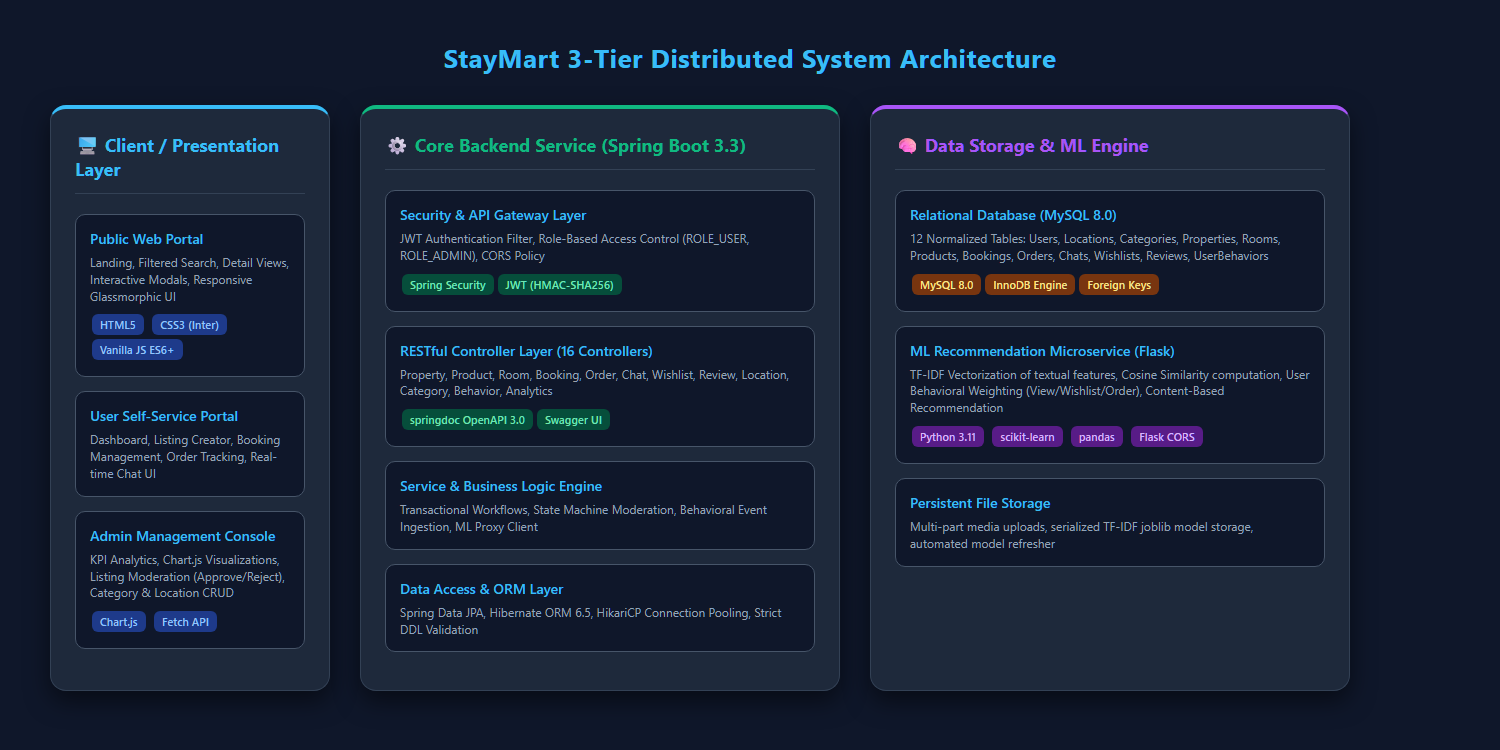
\includegraphics[width=0.95\textwidth]{diagrams/arch_diagram.png}
    \caption{High-Level Distributed Framework of the StayMart Platform}
    \label{fig:framework_overview}
\end{figure}

\begin{enumerate}
    \item \textbf{Zero-Brokerage Direct Connection:} Connects students directly with verified property caretakers and student sellers without middleman commissions, keeping off-campus housing affordable.
    \item \textbf{Verified Photographic Asset Standard:} Listings emphasize authentic photographs of rooms, study desks, and equipment taken by students and caretakers rather than generic stock imagery.
    \item \textbf{Contextual Recommendations:} Combines text similarity matching with user interactions (views, wishlists, and inquiries) to highlight relevant listings near the student's campus.
\end{enumerate}

\section{Organization of the Project Report}
The project report is organized into the following chapters:
\begin{itemize}
    \item \textbf{Chapter 2 (Literature Review):} Evaluates existing classified platforms (OLX, Airbnb, MagicBricks), recommendation algorithms (Content-Based vs. Collaborative Filtering), microservice architecture patterns, and identifies practical gaps in current tools.
    \item \textbf{Chapter 3 (System Requirements and Architecture):} Outlines the Software Requirements Specification (SRS), functional and non-functional requirements, UML diagrams, and Data Flow Diagrams (DFD Level 0, 1, and 2).
    \item \textbf{Chapter 4 (Database Design and Relational Modeling):} Explains the MySQL relational schema, Entity-Relationship (ER) diagrams, normalization analysis (1NF through BCNF), and data dictionaries for all 12 tables.
    \item \textbf{Chapter 5 (Backend and ML Microservice Implementation):} Details the Spring Boot 3.3 (Java 17 LTS) backend, stateless JWT security, the Python TF-IDF recommendation pipeline, and the resilient database fallback mechanism.
    \item \textbf{Chapter 6 (Frontend UI/UX Design System):} Presents the OLX and Amazon-inspired responsive design system, design tokens, and modular client-side JavaScript architecture.
    \item \textbf{Chapter 7 (Verification, Testing and Visual Walkthrough):} Documents testing methodologies, unit/integration test results, automated mobile viewport tests, and an illustrated system walkthrough.
    \item \textbf{Chapter 8 (Deployment, Cloud Hosting and Startup Guide):} Details free-tier cloud deployment on Vercel, Render, and TiDB Serverless, along with a local development runbook.
    \item \textbf{Chapter 9 (Conclusion and Future Scope):} Summarizes project contributions, reflections, limitations, and the future development roadmap.
    \item \textbf{Appendices \& References:} Provide the REST API catalog, data schemas, and academic citations.
\end{itemize}

\chapter{Literature Review}

\section{Introduction}
Online two-sided marketplaces and accommodation networks have transformed commerce by reducing transaction costs and pairing supply with demand. However, multi-category platforms combining long-term student tenancy with consumer re-commerce in non-metropolitan hill geographies present distinct algorithmic, architectural, and socio-technical challenges that remain unaddressed by generic platforms. This chapter surveys commercial solutions, analyzes recommendation algorithms, evaluates architectural paradigms, and formalizes practical research gaps in Uttarakhand.

\section{Survey and Critical Evaluation of Existing Systems}
To establish an empirical baseline, we evaluate benchmark platforms across domain focus, transaction models, moderation, and regional adaptability.

\subsection{OLX and Quikr (General Classifieds)}
Horizontal C2C classifieds suffer from lack of domain specialization. In accommodations, OLX fails to capture essential room sharing capacities, floor numbers, meal plans, electricity rules, curfews, or deposit refund policies. Furthermore, absence of pre-publication moderation produces outdated listings and broker spam.

\subsection{Airbnb and Booking.com (Short-Term Hospitality)}
Airbnb provides polished interfaces and calendar bookings, but its financial structure is built for short-term tourism with daily tariffs and 14\%--20\% service fees. Students in Dehradun require semester leasing without recurring percentage charges. Airbnb also lacks student re-commerce integration.

\subsection{Flatmates and Nestaway (Shared Rental Networks)}
Nestaway operates as a managed real estate company with rigid leases, management premiums, and focus limited to Tier-1 metropolises (Bengaluru, Pune, NCR), maintaining zero operational presence in Uttarakhand educational hubs like Dehradun or Roorkee.

\subsection{MagicBricks and 99acres (Commercial Real Estate)}
These platforms monetize through licensed brokers who purchase lead packs. Students seeking affordable ₹5,000/month rooms near Graphic Era Hill University face aggressive broker calls demanding upfront commissions, defeating direct student-to-owner tenancy.

\begin{table}[htbp]
\centering
\caption{Comparative Feature Matrix: StayMart vs. Existing Commercial Platforms}
\label{tab:comparative_matrix}
\footnotesize
\begin{tabularx}{\textwidth}{lccccc}
\toprule
\textbf{Feature Dimension} & \textbf{OLX} & \textbf{Airbnb} & \textbf{MagicBricks} & \textbf{Nestaway} & \textbf{StayMart (Proposed)} \\
\midrule
Primary Focus & Horizontal C2C & Short-Term Stays & Property Sales & Managed Rental & Student Stays + Re-commerce \\
Hyperlocal Granularity & National & Global / Tourist & Metro Agents & Tier-1 Metros & Uttarakhand Corridors \\
Brokerage / Commission & Variable / Spam & 14\%--20\% & Broker Leads & Monthly Margin & \textbf{Zero Brokerage} \\
Room-Level Inventory & No & Whole Property & No & Managed Beds & \textbf{Yes (Single/Double/Dorm)} \\
Re-commerce Integration & Standalone & None & None & None & \textbf{Yes (Unified Marketplace)} \\
Direct In-App Messaging & Basic & Host Only & Lead Form & Agent Support & \textbf{Yes (Real-Time Peer Chat)} \\
ML Recommendation Engine & Static Search & Collaborative & Keyword Filter & Basic Heuristic & \textbf{TF-IDF + Cosine Hybrid} \\
Listing Pre-Moderation & No (Reactive) & Verified & Agent Filtered & Company Audit & \textbf{Yes (Admin Approval Gate)} \\
Realistic Photographic Standard & Low / Stock & High & Stock Render & Managed Shoot & \textbf{Verified (authentic student/host uploads)} \\
\bottomrule
\end{tabularx}
\end{table}

\section{Theoretical Analysis of Recommendation Algorithms}
Recommender systems predict user preference ratings and surface candidate items from catalogues \cite{resnick1997recommender}. We evaluate Collaborative Filtering against Content-Based and Hybrid approaches to justify StayMart's design.

\subsection{Collaborative Filtering (CF) and Its Regional Limitations}
Collaborative Filtering predicts interest based on historical interaction patterns across users \cite{sarwar2001item}. Pearson Correlation evaluates neighborhood similarity:
\begin{equation}
\text{sim}(u, v) = \frac{\sum_{i \in I_{uv}} (r_{u, i} - \bar{r}_u)(r_{v, i} - \bar{r}_v)}{\sqrt{\sum_{i \in I_{uv}} (r_{u, i} - \bar{r}_u)^2} \sqrt{\sum_{i \in I_{uv}} (r_{v, i} - \bar{r}_v)^2}}
\end{equation}
While effective for dense media catalogues \cite{koren2009matrix}, CF fails in regional classifieds due to three obstacles: (1) \textit{Cold-Start Problem}: new room and item listings have zero historical ratings; (2) \textit{Matrix Sparsity}: localized density typically falls below $0.05\%$; (3) \textit{Inventory Exclusivity}: second-hand goods represent single-inventory assets ($N=1$) that vanish upon purchase.

\subsection{Content-Based Filtering (CBF) and Vector Space Modeling}
Content-Based Filtering evaluates item attribute similarity against user preference profiles \cite{lops2011content}. Each listing is synthesized into an attribute document:
\begin{equation}
d = \text{Title} \oplus \text{Description} \oplus \text{Category} \oplus \text{City} \oplus \text{Area} \oplus \text{PriceTier} \oplus \text{Amenities}
\end{equation}
Term Frequency-Inverse Document Frequency (TF-IDF) weights term importance \cite{salton1988term}:
\begin{equation}
\text{TF}(t, d) = \frac{f_{t, d}}{\sum_{t' \in d} f_{t', d}}, \quad \text{IDF}(t, D) = \log\left(\frac{1 + |D|}{1 + |\{d \in D : t \in d\}|}\right) + 1
\end{equation}
\begin{equation}
w_{t, d} = \text{TF}(t, d) \times \text{IDF}(t, D)
\end{equation}
With $L_2$-normalized vectors ($\|\vec{u}\|_2 = 1$), Cosine Similarity simplifies to the dot product, enabling sub-5ms BLAS computations in scikit-learn \cite{pedregosa2011scikit}:
\begin{equation}
\text{CosineSim}(\vec{u}, \vec{v}) = \vec{u}^T \vec{v}
\end{equation}

\subsection{Hybrid Behavioral Re-Ranking Framework}
To combine content cold-start resilience with user engagement signals, StayMart implements a weighted hybrid re-ranking strategy \cite{burke2002hybrid}. Actions $a_k$ are assigned empirical weights: $\text{VIEW} = 1.0$, $\text{SEARCH} = 2.0$, $\text{WISHLIST} = 3.0$, $\text{CONTACT} = 4.0$, $\text{BOOK/ORDER} = 5.0$. The user profile $\vec{p}_u$ incorporates exponential time decay:
\begin{equation}
\vec{p}_u = \sum_{k=1}^m W(a_k) e^{-\lambda \tau_k} \vec{v}_{i_k}
\end{equation}
The composite recommendation score combines cosine similarity, campus proximity, and popularity:
\begin{equation}
S(u, c) = \alpha \cdot \text{CosineSim}(\vec{p}_u, \vec{v}_c) + \beta \cdot \text{LocalityBonus}(u, C_c) + \gamma \cdot \text{PopularityPrior}(c)
\end{equation}
where $\alpha + \beta + \gamma = 1.0$, ensuring recommendations strictly align with the student's geographic corridor.

\section{Architectural Paradigms: Monolithic vs. Distributed Microservices}
In architecting enterprise web applications, the division of responsibilities across compute boundaries is a pivotal design decision \cite{newman2021building, fielding2000architectural}.

\begin{figure}[htbp]
    \centering
    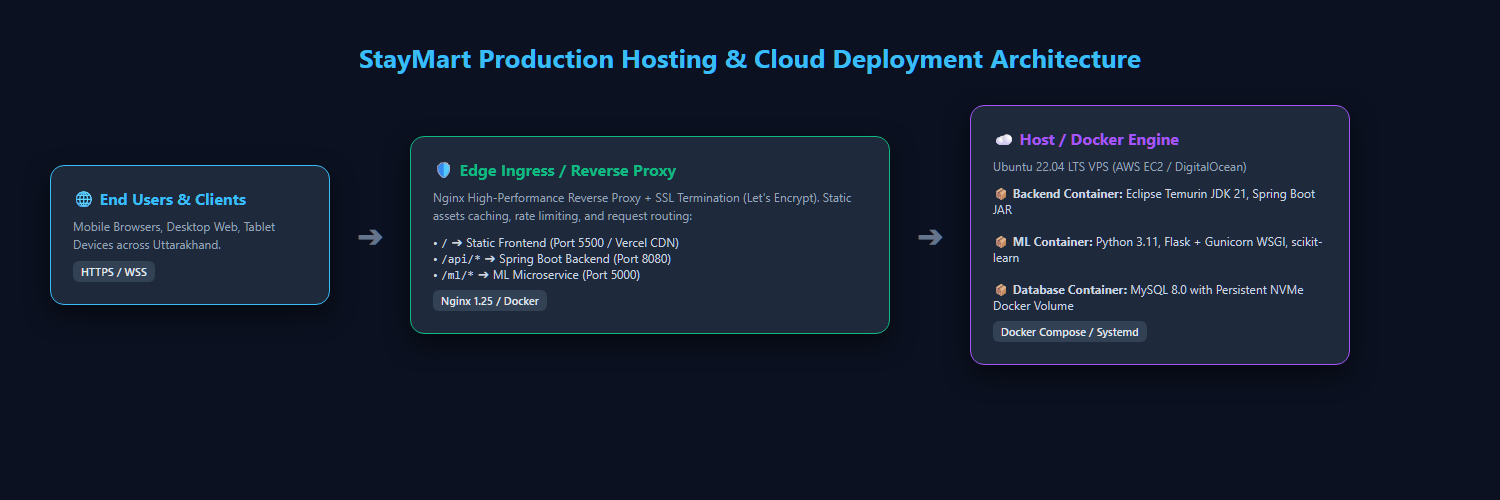
\includegraphics[width=0.92\textwidth]{diagrams/deployment_arch.png}
    \caption{Distributed Microservice Deployment Topology vs. Monolithic Boundaries}
    \label{fig:deployment_topology}
\end{figure}

A monolithic Spring Boot application executes transactional CRUD and intensive ML vector computations within a single JVM. This causes library limitations (Java lacks native scikit-learn parity) and CPU contention during heavy matrix calculations. StayMart adopts a decoupled topology:
\begin{enumerate}
    \item \textbf{Spring Boot 3.3 Core (Port 8080):} Coordinates ACID transactions, JWT authentication, JPA relational entities, and moderation state transitions.
    \item \textbf{Flask ML Microservice (Port 5000):} Operates as an independent service dedicated to TF-IDF transformations, model serialization, and matrix similarity evaluation.
    \item \textbf{Fault-Tolerant Circuit Fallback:} Communication occurs via HTTP REST with 2000ms connect and 3000ms read timeouts. If the ML service is offline, Spring Boot gracefully falls back to database-driven queries matching city and category, eliminating HTTP 500 errors.
\end{enumerate}

\section{Modern Frontend Architectures: Vanilla JS vs. Heavy SPAs}
Modern single-page application (SPA) frameworks (React, Angular) introduce substantial JavaScript payloads (500KB--1.5MB minified) and build fragility, degrading performance on congested campus cellular networks. StayMart intentionally adopts a \textbf{Vanilla HTML5, CSS3, and ES6+ JavaScript} architecture with zero build steps, delivering sub-45 KB payloads, sub-second rendering, and direct static edge deployment on Vercel or CDN nodes.

\section{Identified Practical Gaps and Chapter Summary}
Our systematic review reveals four definitive market gaps: (1) absence of dual-inventory accommodation and re-commerce platforms; (2) lack of Uttarakhand hyperlocal campus granularity; (3) cold-start vulnerability in C2C classifieds; and (4) exploitative brokerage fees. 

In summary, Content-Based TF-IDF vectorization with behavioral re-ranking resolves the sparsity problem, while a decoupled Spring Boot and Flask microservice architecture paired with a lightweight Vanilla JS frontend provides the optimal balance of transactional integrity, ML compute isolation, and mobile performance. The next chapter details system requirements and architectural modeling.

\chapter{System Requirements and High-Level Architecture}

\section{Introduction}
Engineering a resilient, distributed, two-sided marketplace requires structured requirements specification and formal architectural modeling. This chapter establishes the Software Requirements Specification (SRS), non-functional constraints, 3-tier distributed architecture, UML sequence interactions, and operational environments for StayMart.

\section{Software Requirements Specification (SRS)}

\subsection{User Personas and Actor Hierarchy}
StayMart delineates four primary actor classifications interacting within the platform ecosystem:
\begin{enumerate}
    \item \textbf{Guest User:} Unauthenticated visitor with read-only access to approved listings, regional filters, and public categories.
    \item \textbf{Verified Tenant / Buyer:} Registered user authenticated via JWT bearer token with privileges to book rooms, order items, save wishlists, and initiate peer chat.
    \item \textbf{Property Host / Seller:} Authenticated listing author managing room inventories, pricing tiers, deposits, condition notes, and order state transitions.
    \item \textbf{Platform Administrator:} Privileged operator (\texttt{ROLE\_ADMIN}) governing pre-publication moderation, auditing accounts, and viewing telemetry.
\end{enumerate}

\begin{figure}[htbp]
    \centering
    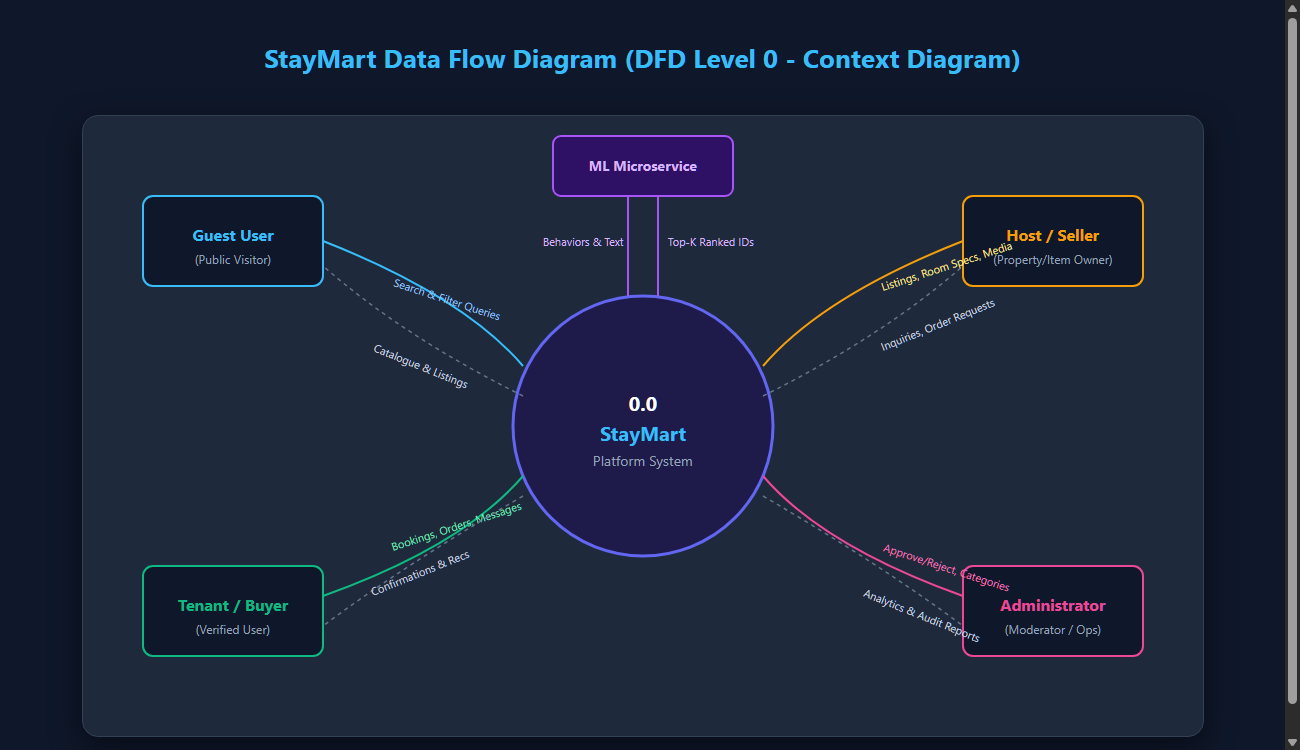
\includegraphics[width=0.92\textwidth]{diagrams/dfd_level0.png}
    \caption{Data Flow Diagram Level 0 (Context Level Diagram) for the StayMart System}
    \label{fig:dfd0}
\end{figure}

\subsection{Functional Requirements (FR)}
The functional scope is structured into eight core modules summarized in Table \ref{tab:functional_reqs}.

\begin{table}[htbp]
\centering
\caption{Comprehensive Functional Requirements Specification}
\label{tab:functional_reqs}
\footnotesize
\begin{tabularx}{\textwidth}{lp{3.8cm}X}
\toprule
\textbf{Module ID} & \textbf{Module Name} & \textbf{Functional Description and Expected System Behavior} \\
\midrule
\textbf{FR-01} & Authentication \& RBAC & Email uniqueness check, BCrypt password hashing ($cost=10$), JWT generation (HMAC-SHA256, 24h expiration), role enforcement (\texttt{ROLE\_USER}, \texttt{ROLE\_ADMIN}). \\
\textbf{FR-02} & Accommodation Mgmt & CRUD operations for 6 property types with amenities, room inventories, security deposits, address mapping, and multi-image JSON payloads. \\
\textbf{FR-03} & Room-Level Inventory & Multi-unit property association with discrete rooms (Single, Double, Triple, Dorm) specifying room number, floor, rent, and vacancy toggles. \\
\textbf{FR-04} & Product Marketplace & CRUD operations for student goods across 10 categories (Sell vs. Rent), capturing condition grading (Brand New to Fair) and wear specifications. \\
\textbf{FR-05} & Lifecycle Transactions & End-to-end booking state machine (\texttt{PENDING} $\rightarrow$ \texttt{CONFIRMED} $\rightarrow$ \texttt{COMPLETED} / \texttt{CANCELLED}) and order decrement workflows. \\
\textbf{FR-06} & Peer-to-Peer Messaging & Real-time bilateral chat between buyers/tenants and sellers/hosts with unread badges and listing context injection. \\
\textbf{FR-07} & ML Recommendations & Asynchronous microservice integration delivering personalized listings, similar item carousels, and top-rated rankings based on telemetry. \\
\textbf{FR-08} & Admin Governance & Pre-publication moderation queue, account deactivation rules, location/category CRUD, and telemetry chart aggregation. \\
\bottomrule
\end{tabularx}
\end{table}

\subsection{Non-Functional Requirements (NFR)}
\begin{enumerate}
    \item \textbf{Performance (NFR-01):} Core read APIs must respond in $t_{\text{resp}} < 50\text{ ms}$; recommendation endpoints must return within $t_{\text{ml}} < 120\text{ ms}$.
    \item \textbf{Security (NFR-02):} BCrypt password hashing, Spring Data JPA parameterized queries preventing SQL injection, output sanitization via \texttt{escapeHtml()}, and stateless JWT tokens.
    \item \textbf{Data Integrity (NFR-03):} Inventory modifications execute within isolated Spring \texttt{@Transactional} boundaries adhering to ACID guarantees.
    \item \textbf{Decoupling (NFR-04):} The ML microservice is isolated from the transactional Spring Boot core, enabling independent horizontal scaling.
    \item \textbf{Usability (NFR-05):} Responsive layouts from 320px (mobile) to 1280px+ (desktop) adhering to WCAG AAA contrast and zero horizontal overflow.
\end{enumerate}

\section{High-Level 3-Tier Distributed Architecture}
StayMart partitions responsibilities across three decoupled distributed tiers:
\begin{enumerate}
    \item \textbf{Presentation Tier (Client Portal):} Vanilla ES6 JavaScript, HTML5, and CSS3 communicating asynchronously over HTTPS via JSON payloads. Stateless JWT tokens are stored in browser storage and transmitted via \texttt{Authorization: Bearer <JWT>} headers.
    \item \textbf{Business Tier (Spring Boot 3.3 Core):} Executing on Eclipse Temurin OpenJDK 17 LTS, this tier implements a Controller-Service-Repository pattern across 16 REST resource controllers, custom \texttt{JwtAuthenticationFilter}, transactional service handlers, and 12 Spring Data JPA repositories.
    \item \textbf{Persistence and ML Tier:} MySQL 8.0 InnoDB provides ACID persistence across 12 normalized tables. A companion Python 3.11 / Flask WSGI service executes TF-IDF vectorization and serves similarity predictions via REST endpoints.
\end{enumerate}

\section{UML Behavioral Modeling: Sequence Diagrams}
Figure \ref{fig:seq_booking} details the complete lifecycle of an accommodation booking transaction across the three tiers.

\begin{figure}[htbp]
    \centering
    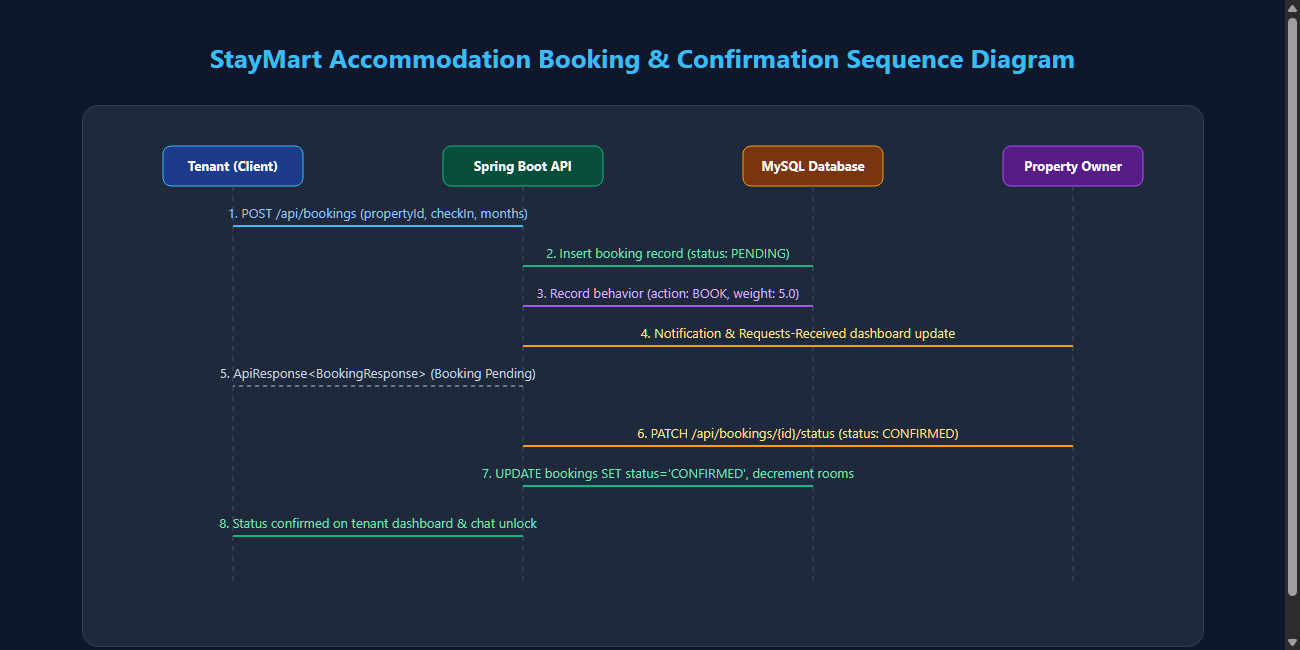
\includegraphics[width=0.92\textwidth]{diagrams/seq_booking.png}
    \caption{UML Sequence Diagram: Accommodation Booking and Confirmation Flow}
    \label{fig:seq_booking}
\end{figure}

The sequence executes through eight calculated stages: (1) tenant submits \texttt{POST /api/bookings}; (2) controller validates JWT and room capacity; (3) service persists booking as \texttt{PENDING}; (4) \texttt{BehaviorService} synchronously logs telemetry ($\text{weight}=5.0$); (5) API returns \texttt{ApiResponse<BookingResponse>} (201 Created); (6) host is alerted via requests dashboard; (7) host submits \texttt{PATCH /api/bookings/\{id\}/status?status=CONFIRMED}; (8) status transitions to \texttt{CONFIRMED}, available bed count decrements, and direct chat is unlocked.

\section{Hardware and Software Operational Environments}
Table \ref{tab:environment_specs} summarizes the operational specifications required to host and execute the StayMart platform.

\begin{table}[htbp]
\centering
\caption{System Hardware and Software Operational Specifications}
\label{tab:environment_specs}
\footnotesize
\begin{tabularx}{\textwidth}{lp{4.2cm}X}
\toprule
\textbf{Layer} & \textbf{Specification Parameter} & \textbf{Recommended Value / Deployment Minimum} \\
\midrule
\multirow{4}{*}{\textbf{Hardware}} & CPU Architecture & x86\_64 (AMD64) or ARM64 (AWS Graviton), 4+ Cores \\
& RAM & 8 GB Minimum (16 GB Recommended for Dockerized Prod) \\
& Storage & 50 GB NVMe SSD (Persistent MySQL Volume + Uploads) \\
& Network & 100 Mbps Full-Duplex Network Interface Card \\
\midrule
\multirow{4}{*}{\textbf{Backend}} & Java Runtime & Eclipse Temurin OpenJDK 17 LTS \\
& Framework & Spring Boot 3.3.5 (Spring Framework 6.1.14) \\
& Build Tool & Apache Maven 3.9.9+ \\
& Embedded Servlet & Apache Tomcat 10.1.31 (HTTP Port 8080) \\
\midrule
\multirow{4}{*}{\textbf{ML Service}} & Python Interpreter & Python 3.11.9+ \\
& Scientific Packages & scikit-learn 1.3.0, pandas 2.0.3, numpy 1.24.4 \\
& Web Framework & Flask 2.3.3 with Flask-CORS 4.0.0 \\
& Production WSGI & Threaded runtime (development) / Gunicorn (Docker) \\
\midrule
\multirow{3}{*}{\textbf{Database}} & Relational Database & MySQL Community Server 8.0.35+ \\
& Storage Engine & InnoDB with UTF8MB4 Character Set \\
& Connection Pool & HikariCP (Maximum Pool Size: 10 Connections) \\
\midrule
\multirow{3}{*}{\textbf{Frontend}} & Client Technologies & Semantic HTML5, CSS3 Custom Properties, JavaScript ES6+ \\
& Visual Rendering & Chart.js 4.4+ (Dashboard Telemetry) \\
& Static Host / Server & Multi-threaded Python server (Dev) / Vercel Edge CDN \\
\bottomrule
\end{tabularx}
\end{table}

\section{Summary}
This chapter formalised the SRS for StayMart across four personas, eight functional modules, and strict performance and security constraints. Through UML sequence modeling and 3-tier decoupling, the interaction contracts were established. The next chapter explores database relational modeling and normalization analysis.

\chapter{Database Design and Relational Modeling}

\section{Introduction}
A marketplace platform handling real-time room bookings, peer-to-peer product orders, in-app chat messages, and student behavioral telemetry requires a dependable relational database. The data persistence layer must guarantee ACID (Atomicity, Consistency, Isolation, Durability) transactions so that rooms and products are never oversold, foreign key constraints are strictly preserved, and queries execute swiftly under concurrent browsing.

StayMart uses \textbf{MySQL 8.0} with the transactional \textbf{InnoDB} storage engine. InnoDB provides row-level locking, foreign key constraint enforcement, and native JSON column support, allowing structured listing attributes (such as amenity lists and photo URLs) to be stored alongside normalized relational data without requiring complex table joins for simple read queries.

This chapter details StayMart's database design:
\begin{enumerate}
    \item Entity-Relationship (ER) modeling and domain relationships.
    \item Data dictionaries for all twelve normalized relational tables.
    \item Normalization analysis demonstrating compliance with 1NF, 2NF, 3NF, and BCNF.
    \item Indexing strategy and referential integrity constraints.
\end{enumerate}

\section{Entity-Relationship (ER) Modeling}
Figure \ref{fig:erd_model} illustrates the complete Entity-Relationship diagram for the StayMart database schema.

\begin{figure}[htbp]
    \centering
    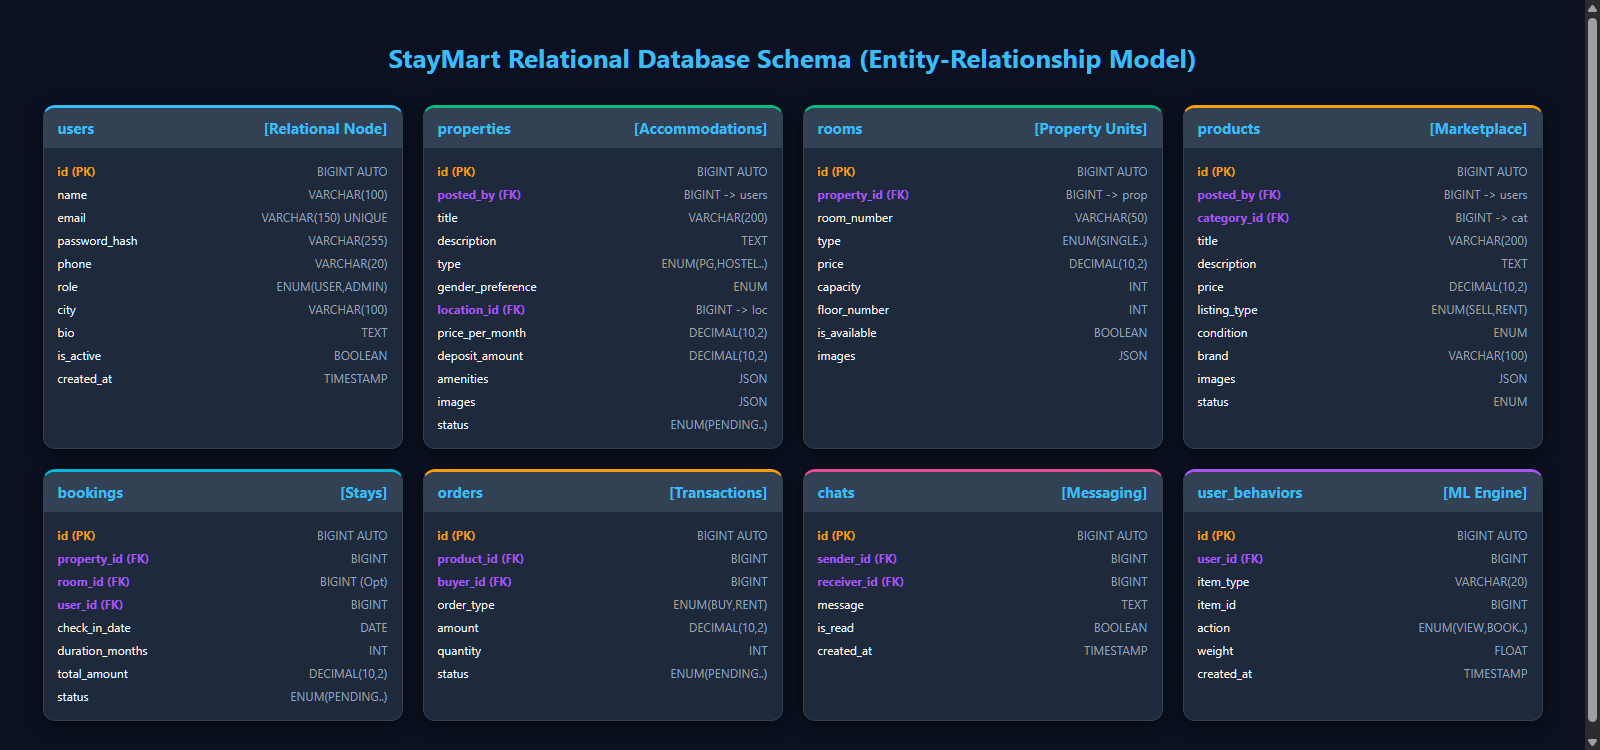
\includegraphics[width=0.98\textwidth]{diagrams/er_diagram.png}
    \caption{Entity-Relationship (ER) Diagram of the StayMart Relational Database Schema}
    \label{fig:erd_model}
\end{figure}

The schema models key relationships across the student marketplace:
\begin{itemize}
    \item \textbf{Users to Properties ($1:N$):} A registered user can list multiple accommodations (\texttt{properties.posted\_by}).
    \item \textbf{Properties to Rooms ($1:N$):} An accommodation contains one or more discrete room configurations (\texttt{rooms.property\_id}) representing single, double, triple, or dormitory beds with individual rent rates.
    \item \textbf{Locations to Listings ($1:N$):} Standardized geographic location records (\texttt{locations.id}) link to properties and products, enforcing consistent city, area, and coordinate data.
    \item \textbf{Categories to Products ($1:N$):} Products belong to hierarchical categories (\texttt{categories.id}) such as Electronics, Mobile Phones, Furniture, Books, and Appliances.
    \item \textbf{Users to Bookings and Orders ($1:N$):} A student submits accommodation bookings (\texttt{bookings.booker\_id}) and classified purchase/rental orders (\texttt{orders.buyer\_id}).
    \item \textbf{Users to Peer Chat ($N:M$ via \texttt{chats}):} Bilateral communication is recorded in \texttt{chats}, linking \texttt{sender\_id} and \texttt{receiver\_id} with listing context.
    \item \textbf{Users to Behavioral Events ($1:N$):} Telemetry events (views, searches, wishlists, booking attempts) are captured in \texttt{user\_behaviors} to train the recommendation engine.
\end{itemize}

\section{Relational Schema Data Dictionaries}
The StayMart schema comprises twelve tables with explicit data types, default values, and foreign key constraints.

\subsection{Table: \texttt{users}}
Stores registered user accounts, contact information, role assignments, and profile details.
\begin{table}[htbp]
\centering
\caption{Data Dictionary: \texttt{users} Table}
\label{tab:dict_users}
\footnotesize
\begin{tabularx}{\textwidth}{lp{2.8cm}lp{2.2cm}X}
\toprule
\textbf{Column Name} & \textbf{Data Type} & \textbf{Nullability} & \textbf{Default} & \textbf{Description} \\
\midrule
\texttt{id} & \texttt{BIGINT} & NOT NULL & AUTO\_INCR & Primary Key, unique user identifier. \\
\texttt{name} & \texttt{VARCHAR(100)} & NOT NULL & None & Full name of the student or property host. \\
\texttt{email} & \texttt{VARCHAR(150)} & NOT NULL & None & Unique login email address. \\
\texttt{password\_hash} & \texttt{VARCHAR(255)} & NOT NULL & None & BCrypt password hash ($cost=10$). \\
\texttt{phone} & \texttt{VARCHAR(15)} & NULL & NULL & Contact phone number for inquiries. \\
\texttt{role} & \texttt{ENUM} & NOT NULL & 'USER' & Role: \texttt{USER} or \texttt{ADMIN}. \\
\texttt{city} & \texttt{VARCHAR(100)} & NULL & 'Dehradun' & Primary campus city in Uttarakhand. \\
\texttt{state} & \texttt{VARCHAR(100)} & NULL & 'Uttarakhand' & State jurisdiction. \\
\texttt{bio} & \texttt{TEXT} & NULL & NULL & User bio or caretaker description. \\
\texttt{profile\_pic} & \texttt{VARCHAR(255)} & NULL & NULL & Relative or remote URL to avatar image. \\
\texttt{is\_active} & \texttt{BOOLEAN} & NOT NULL & TRUE & Account active/suspended flag. \\
\texttt{is\_verified} & \texttt{BOOLEAN} & NOT NULL & FALSE & Verification badge indicator. \\
\texttt{created\_at} & \texttt{TIMESTAMP} & NOT NULL & CURRENT\_TS & Account creation timestamp. \\
\bottomrule
\end{tabularx}
\end{table}

\subsection{Table: \texttt{locations}}
Geographic taxonomy representing cities and student campus clusters across Uttarakhand.
\begin{table}[htbp]
\centering
\caption{Data Dictionary: \texttt{locations} Table}
\label{tab:dict_locations}
\footnotesize
\begin{tabularx}{\textwidth}{lp{2.8cm}lp{2.2cm}X}
\toprule
\textbf{Column Name} & \textbf{Data Type} & \textbf{Nullability} & \textbf{Default} & \textbf{Description} \\
\midrule
\texttt{id} & \texttt{BIGINT} & NOT NULL & AUTO\_INCR & Primary Key, location identifier. \\
\texttt{city} & \texttt{VARCHAR(100)} & NOT NULL & None & City name (e.g., Dehradun, Rishikesh, Roorkee). \\
\texttt{area} & \texttt{VARCHAR(100)} & NULL & NULL & Specific campus locality (e.g., Clement Town). \\
\texttt{state} & \texttt{VARCHAR(100)} & NULL & 'Uttarakhand' & State name. \\
\texttt{pincode} & \texttt{VARCHAR(10)} & NULL & NULL & Postal code. \\
\texttt{latitude} & \texttt{DECIMAL(10,8)} & NULL & NULL & Latitude coordinate. \\
\texttt{longitude} & \texttt{DECIMAL(11,8)} & NULL & NULL & Longitude coordinate. \\
\bottomrule
\end{tabularx}
\end{table}

\subsection{Table: \texttt{categories}}
Product and accommodation taxonomy organizing listings into intuitive browsing buckets.
\begin{table}[htbp]
\centering
\caption{Data Dictionary: \texttt{categories} Table}
\label{tab:dict_categories}
\footnotesize
\begin{tabularx}{\textwidth}{lp{2.8cm}lp{2.2cm}X}
\toprule
\textbf{Column Name} & \textbf{Data Type} & \textbf{Nullability} & \textbf{Default} & \textbf{Description} \\
\midrule
\texttt{id} & \texttt{BIGINT} & NOT NULL & AUTO\_INCR & Primary Key, category identifier. \\
\texttt{name} & \texttt{VARCHAR(100)} & NOT NULL & None & Category name (e.g., Electronics, Furniture). \\
\texttt{type} & \texttt{ENUM} & NOT NULL & None & Category type: \texttt{ACCOMMODATION} or \texttt{PRODUCT}. \\
\texttt{icon} & \texttt{VARCHAR(50)} & NULL & NULL & Icon identifier or CSS class name. \\
\texttt{parent\_id} & \texttt{BIGINT} & NULL & NULL & Foreign Key $\rightarrow$ \texttt{categories(id)} (self-reference). \\
\bottomrule
\end{tabularx}
\end{table}

\subsection{Table: \texttt{properties}}
Rental accommodation listings including PGs, hostels, shared flats, and rooms.
\begin{table}[htbp]
\centering
\caption{Data Dictionary: \texttt{properties} Table}
\label{tab:dict_properties}
\footnotesize
\begin{tabularx}{\textwidth}{lp{2.8cm}lp{2.2cm}X}
\toprule
\textbf{Column Name} & \textbf{Data Type} & \textbf{Nullability} & \textbf{Default} & \textbf{Description} \\
\midrule
\texttt{id} & \texttt{BIGINT} & NOT NULL & AUTO\_INCR & Primary Key, property listing ID. \\
\texttt{posted\_by} & \texttt{BIGINT} & NOT NULL & None & Foreign Key $\rightarrow$ \texttt{users(id)}. \\
\texttt{title} & \texttt{VARCHAR(200)} & NOT NULL & None & Listing headline. \\
\texttt{description} & \texttt{TEXT} & NULL & NULL & Detailed property description and rules. \\
\texttt{type} & \texttt{ENUM} & NOT NULL & None & PG, ROOM, HOSTEL, HOTEL, FLAT, DORMITORY. \\
\texttt{gender\_preference}& \texttt{ENUM} & NOT NULL & 'ANY' & MALE, FEMALE, or ANY. \\
\texttt{address} & \texttt{VARCHAR(255)} & NULL & NULL & Street address or landmark. \\
\texttt{area} & \texttt{VARCHAR(100)} & NULL & NULL & Local campus area name. \\
\texttt{location\_id} & \texttt{BIGINT} & NULL & NULL & Foreign Key $\rightarrow$ \texttt{locations(id)}. \\
\texttt{price\_per\_month}& \texttt{DECIMAL(10,2)}& NULL & NULL & Base monthly rental rate (INR). \\
\texttt{deposit\_amount} & \texttt{DECIMAL(10,2)}& NOT NULL & 0.00 & Refundable security deposit. \\
\texttt{amenities} & \texttt{JSON} & NULL & NULL & JSON array of amenities (WiFi, Power Backup, Meals). \\
\texttt{total\_rooms} & \texttt{INT} & NOT NULL & 1 & Total capacity / rooms in listing. \\
\texttt{available\_rooms}& \texttt{INT} & NOT NULL & 1 & Currently vacant rooms/beds. \\
\texttt{images} & \texttt{JSON} & NULL & NULL & JSON array of photograph URLs. \\
\texttt{status} & \texttt{ENUM} & NOT NULL & 'PENDING' & PENDING, APPROVED, or REJECTED. \\
\texttt{is\_available} & \texttt{BOOLEAN} & NOT NULL & TRUE & Active availability toggle. \\
\texttt{created\_at} & \texttt{TIMESTAMP} & NOT NULL & CURRENT\_TS & Publication timestamp. \\
\bottomrule
\end{tabularx}
\end{table}

\subsection{Table: \texttt{rooms}}
Individual room configurations within an accommodation property.
\begin{table}[htbp]
\centering
\caption{Data Dictionary: \texttt{rooms} Table}
\label{tab:dict_rooms}
\footnotesize
\begin{tabularx}{\textwidth}{lp{2.8cm}lp{2.2cm}X}
\toprule
\textbf{Column Name} & \textbf{Data Type} & \textbf{Nullability} & \textbf{Default} & \textbf{Description} \\
\midrule
\texttt{id} & \texttt{BIGINT} & NOT NULL & AUTO\_INCR & Primary Key, room identifier. \\
\texttt{property\_id} & \texttt{BIGINT} & NOT NULL & None & Foreign Key $\rightarrow$ \texttt{properties(id)}. \\
\texttt{room\_number} & \texttt{VARCHAR(20)} & NULL & NULL & Room number or identifier label. \\
\texttt{type} & \texttt{ENUM} & NOT NULL & None & SINGLE, DOUBLE, TRIPLE, or DORMITORY. \\
\texttt{price} & \texttt{DECIMAL(10,2)}& NULL & NULL & Monthly rent for this room configuration. \\
\texttt{capacity} & \texttt{INT} & NOT NULL & 1 & Maximum number of student occupants. \\
\texttt{floor\_number} & \texttt{INT} & NOT NULL & 0 & Floor number within building. \\
\texttt{is\_available} & \texttt{BOOLEAN} & NOT NULL & TRUE & Availability status of room. \\
\texttt{images} & \texttt{JSON} & NULL & NULL & JSON array of room-specific photos. \\
\bottomrule
\end{tabularx}
\end{table}

\subsection{Table: \texttt{products}}
Marketplace listings for second-hand student gear posted for sale or rent.
\begin{table}[htbp]
\centering
\caption{Data Dictionary: \texttt{products} Table}
\label{tab:dict_products}
\footnotesize
\begin{tabularx}{\textwidth}{lp{2.8cm}lp{2.2cm}X}
\toprule
\textbf{Column Name} & \textbf{Data Type} & \textbf{Nullability} & \textbf{Default} & \textbf{Description} \\
\midrule
\texttt{id} & \texttt{BIGINT} & NOT NULL & AUTO\_INCR & Primary Key, product listing ID. \\
\texttt{posted\_by} & \texttt{BIGINT} & NOT NULL & None & Foreign Key $\rightarrow$ \texttt{users(id)}. \\
\texttt{category\_id} & \texttt{BIGINT} & NULL & NULL & Foreign Key $\rightarrow$ \texttt{categories(id)}. \\
\texttt{title} & \texttt{VARCHAR(200)} & NOT NULL & None & Item headline (e.g., Symphony Cooler). \\
\texttt{description} & \texttt{TEXT} & NULL & NULL & Item condition, specifications, and reason for selling. \\
\texttt{price} & \texttt{DECIMAL(10,2)}& NOT NULL & None & Asking price or rental rate (INR). \\
\texttt{listing\_type} & \texttt{ENUM} & NOT NULL & 'SELL' & SELL, RENT, or BOTH. \\
\texttt{condition} & \texttt{ENUM} & NOT NULL & 'GOOD' & NEW, LIKE\_NEW, GOOD, FAIR, or OLD. \\
\texttt{brand} & \texttt{VARCHAR(100)} & NULL & NULL & Manufacturer or brand name. \\
\texttt{location\_id} & \texttt{BIGINT} & NULL & NULL & Foreign Key $\rightarrow$ \texttt{locations(id)}. \\
\texttt{area} & \texttt{VARCHAR(100)} & NULL & NULL & Campus area or pickup neighborhood. \\
\texttt{images} & \texttt{JSON} & NULL & NULL & JSON array of authentic item photos. \\
\texttt{status} & \texttt{ENUM} & NOT NULL & 'PENDING' & PENDING, APPROVED, or REJECTED. \\
\texttt{is\_available} & \texttt{BOOLEAN} & NOT NULL & TRUE & Inventory flag (active vs. sold). \\
\texttt{views\_count} & \texttt{INT} & NOT NULL & 0 & Popularity view counter. \\
\texttt{created\_at} & \texttt{TIMESTAMP} & NOT NULL & CURRENT\_TS & Publication timestamp. \\
\bottomrule
\end{tabularx}
\end{table}

\subsection{Tables: \texttt{bookings}, \texttt{orders}, \texttt{wishlists}, \texttt{reviews}, \texttt{chats}, and \texttt{user\_behaviors}}
The remaining transactional and interaction tables are structured as follows:

\begin{itemize}
    \item \textbf{\texttt{bookings}:} Captures accommodation reservations. Foreign keys: \texttt{booker\_id} $\rightarrow$ \texttt{users(id)}, \texttt{property\_id} $\rightarrow$ \texttt{properties(id)}, and optional \texttt{room\_id} $\rightarrow$ \texttt{rooms(id)}. Columns include \texttt{check\_in} (DATE), \texttt{check\_out} (DATE), \texttt{months} (INT), \texttt{total\_amount} (DECIMAL), \texttt{status} (\texttt{PENDING}, \texttt{CONFIRMED}, \texttt{CANCELLED}, \texttt{COMPLETED}), and \texttt{message} (TEXT).
    \item \textbf{\texttt{orders}:} Captures classified product purchases and rentals. Foreign keys: \texttt{buyer\_id} $\rightarrow$ \texttt{users(id)}, \texttt{seller\_id} $\rightarrow$ \texttt{users(id)}, and \texttt{product\_id} $\rightarrow$ \texttt{products(id)}. Columns include \texttt{quantity} (INT), \texttt{amount} (DECIMAL), \texttt{order\_type} (\texttt{BUY} or \texttt{RENT}), \texttt{rent\_start} (DATE), \texttt{rent\_end} (DATE), \texttt{status}, and \texttt{message}.
    \item \textbf{\texttt{wishlists}:} Manages saved student bookmarks. Foreign key: \texttt{user\_id} $\rightarrow$ \texttt{users(id)}. Columns include \texttt{item\_type} (\texttt{PROPERTY} or \texttt{PRODUCT}), \texttt{item\_id} (BIGINT), and a unique constraint on \texttt{(user\_id, item\_type, item\_id)} preventing duplicate bookmarks.
    \item \textbf{\texttt{reviews}:} Stores student ratings and feedback after confirmed stays or purchases. Foreign key: \texttt{reviewer\_id} $\rightarrow$ \texttt{users(id)}. Columns include \texttt{item\_type} (\texttt{PROPERTY}, \texttt{PRODUCT}, or \texttt{USER}), \texttt{item\_id} (BIGINT), \texttt{rating} (INT, constrained between 1 and 5), and \texttt{comment} (TEXT).
    \item \textbf{\texttt{chats}:} Records direct peer-to-peer messages between students and hosts. Foreign keys: \texttt{sender\_id} $\rightarrow$ \texttt{users(id)} and \texttt{receiver\_id} $\rightarrow$ \texttt{users(id)}. Columns include \texttt{listing\_type}, \texttt{listing\_id}, \texttt{message} (TEXT), \texttt{is\_read} (BOOLEAN), and \texttt{timestamp}.
    \item \textbf{\texttt{user\_behaviors}:} Records user telemetry for recommendation model training. Foreign key: \texttt{user\_id} $\rightarrow$ \texttt{users(id)}. Columns include \texttt{item\_type}, \texttt{item\_id}, \texttt{action} (\texttt{VIEW}, \texttt{SEARCH}, \texttt{WISHLIST}, \texttt{BOOK}, \texttt{ORDER}, \texttt{CONTACT}), \texttt{search\_query}, \texttt{city\_filter}, and \texttt{timestamp}.
\end{itemize}

\section{Database Normalization Analysis}
To eliminate data redundancy and prevent insertion, update, and deletion anomalies, we evaluate the schema through formal normalization stages.

\subsection{First Normal Form (1NF)}
A relation satisfies 1NF if all attribute domains contain only atomic, indivisible values, and there are no repeating groups.
\begin{itemize}
    \item Every column in StayMart—such as \texttt{price}, \texttt{name}, \texttt{email}, and \texttt{status}—contains atomic scalar values.
    \item \textbf{Use of JSON Attributes:} Columns like \texttt{amenities} and \texttt{images} in \texttt{properties} and \texttt{products} store JSON arrays. Under MySQL 8.0, the native \texttt{JSON} type functions as an atomic document datatype. Storing image URLs and amenity tags as serialized collections attached to a single listing avoids maintaining separate join tables for static arrays while strictly preserving 1NF.
\end{itemize}

\subsection{Second Normal Form (2NF)}
A relation is in 2NF if it is in 1NF and every non-prime attribute is fully functionally dependent on the entire primary key (no partial key dependencies).
\begin{itemize}
    \item Every table in StayMart uses a single-column surrogate primary key (\texttt{id BIGINT AUTO\_INCREMENT}).
    \item Because every candidate key consists of exactly one attribute ($K = \{\text{id}\}$), a partial dependency on a subset of a composite key is impossible. Therefore, all twelve tables satisfy 2NF unconditionally.
\end{itemize}

\subsection{Third Normal Form (3NF)}
A relation is in 3NF if it is in 2NF and no non-prime attribute is transitively dependent on the primary key. Formally, for every non-trivial functional dependency $X \rightarrow Y$, either $X$ is a superkey or $Y$ is a prime attribute.

\textbf{Practical Case Study: Geographical Normalization (\texttt{locations})} \\
Consider an unnormalized property table containing city, area, and pincode directly:
\begin{equation}
\text{PropertyID} \rightarrow \{\text{Area}, \text{City}, \text{State}, \text{Pincode}\}
\end{equation}
This design introduces transitive dependencies because:
\begin{equation}
\text{PropertyID} \rightarrow \text{Pincode} \quad \text{and} \quad \text{Pincode} \rightarrow \{\text{City}, \text{State}\}
\end{equation}
This causes three classic database anomalies:
\begin{enumerate}
    \item \textbf{Redundancy:} Every student PG in Clement Town would duplicate the string ``Clement Town, Dehradun, Uttarakhand, 248002''.
    \item \textbf{Update Anomaly:} Changing a locality name requires updating hundreds of individual property rows.
    \item \textbf{Deletion Anomaly:} Deleting all listings in a new campus locality would delete the knowledge that the locality exists in the database.
\end{enumerate}

StayMart eliminates this transitive dependency by isolating geographic data into the \texttt{locations} relation. Properties reference \texttt{location\_id} as a foreign key. Thus, all non-prime attributes in \texttt{properties} depend directly on the primary key, satisfying 3NF.

\subsection{Boyce-Codd Normal Form (BCNF)}
A relation is in BCNF if for every non-trivial functional dependency $X \rightarrow Y$, $X$ is a superkey. In StayMart, all non-trivial functional dependencies originate from primary keys (\texttt{id}) or unique candidate keys (such as \texttt{users.email}), which are verified superkeys. Therefore, the schema satisfies BCNF.

\section{Indexing Strategy and Referential Integrity}
To ensure fast query execution across thousands of student listings, B-Tree indexes are defined on foreign keys and search filter columns:

\begin{enumerate}
    \item \textbf{Foreign Key Indexes:} Indexes on \texttt{properties(posted\_by)}, \texttt{properties(location\_id)}, \texttt{products(category\_id)}, \texttt{bookings(property\_id)}, and \texttt{orders(product\_id)} ensure that relational joins execute efficiently via index range scans rather than full table scans.
    \item \textbf{Search Filter Indexes:} The public catalog search frequently filters by approval status and availability. Composite indexes on \texttt{(status, is\_available, created\_at)} allow MySQL to filter approved listings directly from the index tree.
    \item \textbf{Telemetry Stream Indexes:} The \texttt{user\_behaviors} table receives high write volume. An index on \texttt{(user\_id, created\_at)} allows the recommendation service to retrieve a user's recent interactions in milliseconds.
\end{enumerate}

\section{Summary}
This chapter presented the database design of StayMart, detailing the twelve relational tables, ER modeling, normalization proofs, and indexing strategy. The use of MySQL 8.0 with InnoDB guarantees transactional consistency for room bookings and product orders, while native JSON columns efficiently handle media assets and amenity tags. The following chapter details the backend implementation and machine learning recommendation microservice.

\chapter{Backend and Machine Learning Microservice Implementation}

\section{Introduction}
StayMart's backend architecture is designed around a decoupled multi-tier setup that separates core transactional business operations from machine learning analytics:
\begin{enumerate}
    \item \textbf{Spring Boot 3.3 Core Backend (Java 17 LTS):} Handles user authentication, rental bookings, marketplace orders, peer messaging, and administrative moderation using strongly typed Java services and Spring Data JPA.
    \item \textbf{Python 3.11 / Flask Machine Learning Microservice:} An asynchronous microservice responsible for text preprocessing, Term Frequency-Inverse Document Frequency (TF-IDF) feature vectorization, and cosine similarity ranking.
\end{enumerate}

This chapter details the technical implementation, design patterns, security pipelines, and algorithm workflows across both backend services.

\section{Spring Boot Core Backend Architecture}
The core backend is built on Spring Boot 3.3.5 and Spring Framework 6.1.14 running on Java 17 LTS. The application uses modern Java language features—including immutable record classes for Data Transfer Objects (DTOs), text blocks for readable queries, enhanced switch expressions, and pattern matching for instanceof—alongside standard thread-pool request execution on embedded Apache Tomcat.

\subsection{Architectural Layering: Controller-Service-Repository Pattern}
The backend organizes business logic through the standard Controller-Service-Repository pattern:

\begin{figure}[htbp]
    \centering
    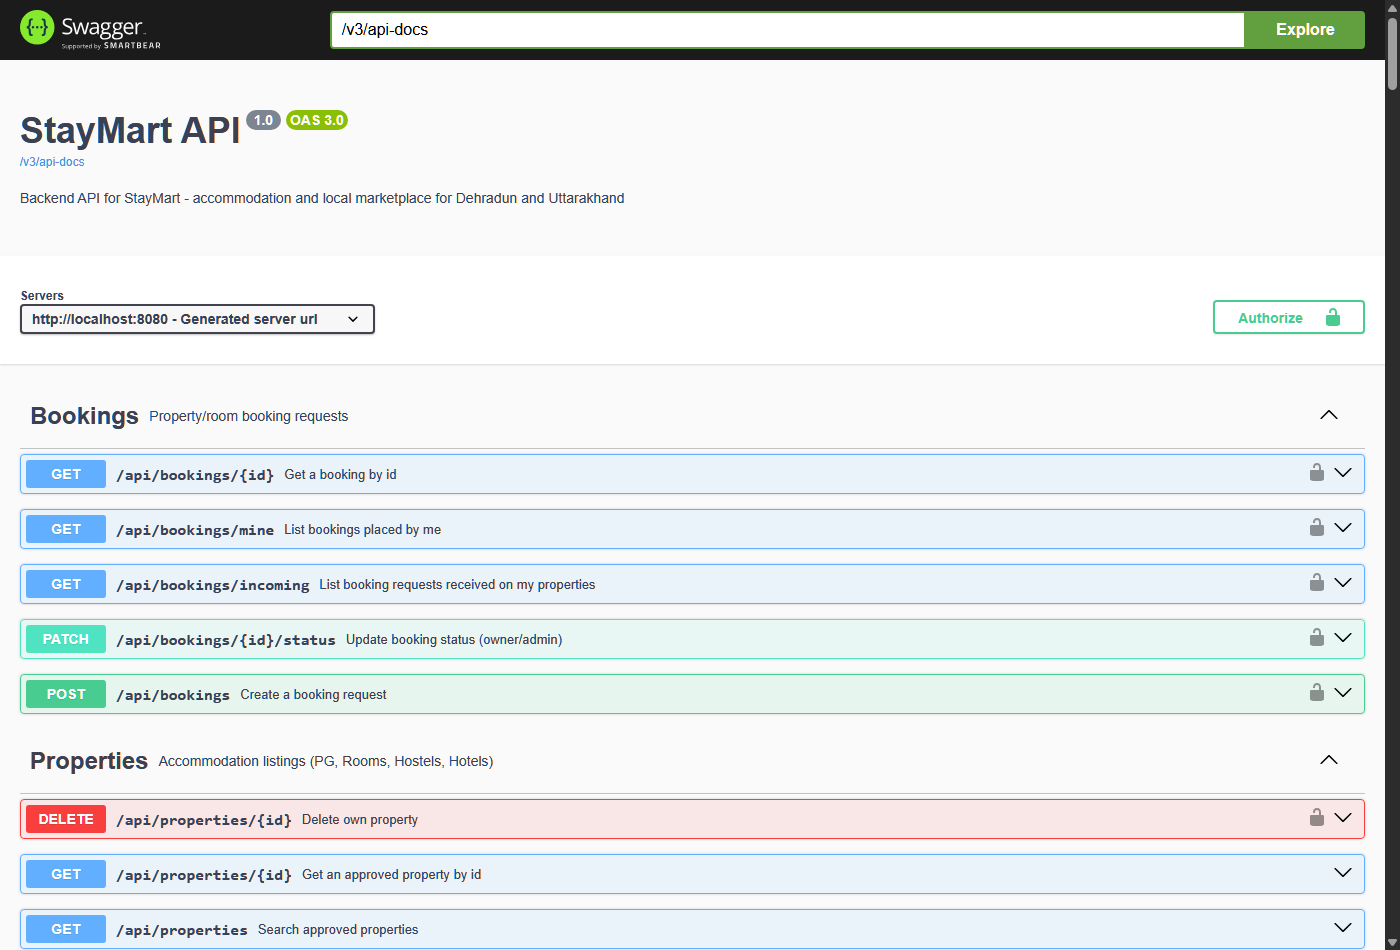
\includegraphics[width=0.95\textwidth]{screenshots/swagger_api.png}
    \caption{Springdoc OpenAPI 3.0 Swagger UI Exposing Core Backend REST Endpoints}
    \label{fig:swagger_api}
\end{figure}

The 16 REST controllers in \texttt{src/main/java/com/staymart/controller/} are organized into four functional groups:
\begin{enumerate}
    \item \textbf{Identity and Profile Management:} \texttt{AuthController} (registration and login), \texttt{UserController} (profile management and verification), and \texttt{FileController} (photograph asset uploads).
    \item \textbf{Accommodation and Inventory:} \texttt{PropertyController} (PG, hostel, and flat listings), \texttt{RoomController} (room configurations and capacities), and \texttt{LocationController} (Uttarakhand campus clusters).
    \item \textbf{Campus Classifieds:} \texttt{ProductController} (student gear listings for sale or rent) and \texttt{CategoryController} (marketplace taxonomy).
    \item \textbf{Interactions and Administration:} \texttt{BookingController} (accommodation reservations), \texttt{OrderController} (product acquisitions), \texttt{ChatController} (in-app student messaging), \texttt{ReviewController} (ratings and feedback), \texttt{WishlistController} (saved listings), \texttt{BehaviorController} (user telemetry events), \texttt{RecommendationController} (personalized and trending feeds), and \texttt{AdminController} (listing moderation and user management).
\end{enumerate}

\subsection{Standardized API Envelope Pattern}
To ensure client applications receive predictable payload structures regardless of success or failure states, all endpoints emit an \texttt{ApiResponse<T>} envelope:

\begin{lstlisting}[language=Java, caption={Generic API Response Wrapper}]
public class ApiResponse<T> {
    private boolean success;
    private String message;
    private T data;
    private Long timestamp;

    public static <T> ApiResponse<T> ok(T data) {
        return new ApiResponse<>(true, "Success", data, System.currentTimeMillis());
    }

    public static <T> ApiResponse<T> ok(String message, T data) {
        return new ApiResponse<>(true, message, data, System.currentTimeMillis());
    }

    public static <T> ApiResponse<T> error(String message) {
        return new ApiResponse<>(false, message, null, System.currentTimeMillis());
    }
}
\end{lstlisting}

Pagination responses encapsulate content lists alongside cursor metadata via \texttt{PageResponse<T>}:
\begin{lstlisting}[language=Java, caption={Paginated Response Wrapper}]
public record PageResponse<T>(
    List<T> content,
    int page,
    int size,
    long totalElements,
    int totalPages,
    boolean last
) {
    public static <T> PageResponse<T> from(Page<T> springPage) {
        return new PageResponse<>(
            springPage.getContent(),
            springPage.getNumber(),
            springPage.getSize(),
            springPage.getTotalElements(),
            springPage.getTotalPages(),
            springPage.isLast()
        );
    }
}
\end{lstlisting}

\section{Security Architecture: Spring Security and Stateless JWT}
Security in StayMart is managed by Spring Security 6, enforcing stateless authentication using JSON Web Tokens (JWT) to avoid server-side session overhead.

\subsection{JWT Signing and Roles}
Upon successful login via \texttt{POST /api/auth/login}, the \texttt{JwtTokenProvider} generates a signed token:
\begin{itemize}
    \item \textbf{Algorithm:} HMAC-SHA256 (\texttt{HS256}) using a 256-bit secret key.
    \item \textbf{Token Claims:} Subject (\texttt{email}), User ID (\texttt{id}), Role authority (\texttt{ROLE\_USER} or \texttt{ROLE\_ADMIN}), Issue time (\texttt{iat}), and Expiration (\texttt{exp}, 24 hours).
\end{itemize}

\subsection{JWT Authentication Filter}
Every inbound HTTP request passes through \texttt{JwtAuthenticationFilter} before reaching the servlet dispatcher:

\begin{lstlisting}[language=Java, caption={JwtAuthenticationFilter Request Interceptor}]
@Component
public class JwtAuthenticationFilter extends OncePerRequestFilter {

    private final JwtTokenProvider tokenProvider;
    private final CustomUserDetailsService userDetailsService;

    @Override
    protected void doFilterInternal(HttpServletRequest request,
                                    HttpServletResponse response,
                                    FilterChain filterChain) throws ServletException, IOException {
        String token = resolveToken(request);
        if (StringUtils.hasText(token) && tokenProvider.validateToken(token)) {
            String email = tokenProvider.getEmailFromToken(token);
            UserDetails userDetails = userDetailsService.loadUserByUsername(email);
            
            UsernamePasswordAuthenticationToken authentication =
                new UsernamePasswordAuthenticationToken(userDetails, null, userDetails.getAuthorities());
            authentication.setDetails(new WebAuthenticationDetailsSource().buildDetails(request));
            
            SecurityContextHolder.getContext().setAuthentication(authentication);
        }
        filterChain.doFilter(request, response);
    }

    private String resolveToken(HttpServletRequest request) {
        String bearer = request.getHeader("Authorization");
        if (StringUtils.hasText(bearer) && bearer.startsWith("Bearer ")) {
            return bearer.substring(7);
        }
        return null;
    }
}
\end{lstlisting}

\subsection{Accurate Security Boundaries}
Each security concern is handled at the appropriate architectural layer:
\begin{itemize}
    \item \textbf{Password Encryption:} Passwords are encrypted with BCrypt ($cost=10$) before database persistence.
    \item \textbf{Authentication and RBAC:} JWT tokens provide stateless session verification and role enforcement. Standard users have access to personal bookings, chats, and listings, while admin routes require \texttt{ROLE\_ADMIN}.
    \item \textbf{SQL Injection Defense:} Provided by Spring Data JPA and Hibernate ORM parameterized queries (\texttt{PreparedStatements}), which treat user inputs strictly as literal parameters.
    \item \textbf{XSS Defense:} Handled by frontend output sanitization via \texttt{escapeHtml()} in \texttt{utils.js} and input validation annotations in Spring Boot DTOs.
\end{itemize}

\section{Machine Learning Recommendation Microservice}
The recommendation microservice is implemented in Python 3.11 with Flask in \texttt{ml-service/}, using scikit-learn for TF-IDF vector transformations.

\subsection{Feature Vectorization and Model Pipeline}
For each listing, the service synthesizes a composite text document concatenating title, description, category, campus area, city, amenities, and price tier buckets:

\begin{lstlisting}[language=Python, caption={Property Text Document Synthesis in recommender.py}]
def build_property_document(row):
    tokens = [
        str(row['title']),
        str(row['description']),
        str(row['type']),
        str(row['gender_preference']),
        str(row['area']),
        str(row['city']),
        " ".join(json.loads(row['amenities'])) if row['amenities'] else ""
    ]
    price = float(row['price_per_month'])
    if price < 5000:
        tokens.append("budget_tier_low")
    elif price <= 10000:
        tokens.append("budget_tier_medium")
    else:
        tokens.append("budget_tier_premium")
    return " ".join(tokens)
\end{lstlisting}

The composite corpus is transformed into a continuous vector space using \texttt{TfidfVectorizer} with unigrams and bigrams $(1, 2)$, sublinear term frequency scaling, and English stop-word filtering. Cosine similarity calculates relevance scores:
\begin{equation}
\text{Similarity}(\vec{u}, \vec{v}) = \frac{\vec{u} \cdot \vec{v}}{\|\vec{u}\|_2 \|\vec{v}\|_2}
\end{equation}

\begin{figure}[htbp]
    \centering
    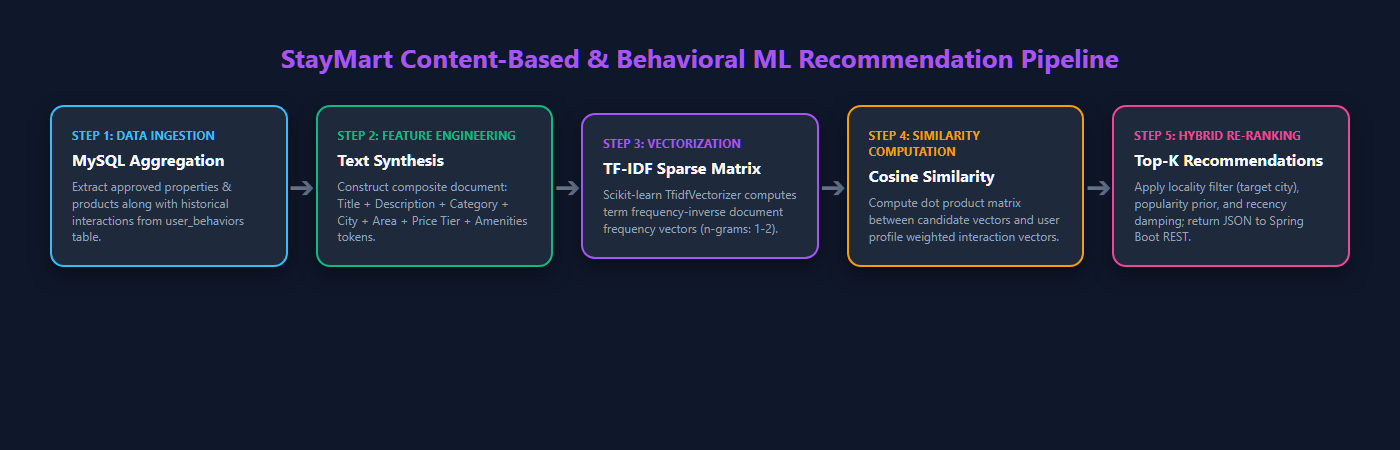
\includegraphics[width=0.92\textwidth]{diagrams/ml_pipeline.png}
    \caption{Machine Learning Content-Based Recommendation Pipeline with TF-IDF Vectorization}
    \label{fig:ml_pipeline}
\end{figure}

\section{Fault-Tolerant Fallback Integration in Spring Boot}
The Spring Boot backend interacts with the Flask ML microservice through \texttt{MlServiceClient}. To ensure platform availability when the ML service is offline or starting up, \texttt{MlServiceClient} configures a 2000ms connection timeout and a 3000ms read timeout:

\begin{lstlisting}[language=Java, caption={Timeout Configuration in MlServiceClient.java}]
SimpleClientHttpRequestFactory requestFactory = new SimpleClientHttpRequestFactory();
requestFactory.setConnectTimeout(2000); // 2000ms connect timeout
requestFactory.setReadTimeout(3000);    // 3000ms read timeout
this.client = builder.baseUrl(mlBaseUrl).requestFactory(requestFactory).build();
\end{lstlisting}

If the ML microservice throws a \texttt{RestClientException} or returns an unparseable response, \texttt{MlServiceClient} catches the exception, logs a warning, and returns an empty list.

The \texttt{RecommendationService} detects this empty list and immediately falls back to approved database listings:

\begin{lstlisting}[language=Java, caption={Resilient Database Fallback in RecommendationService.java}]
@Service
public class RecommendationService {

    private final MlServiceClient mlServiceClient;
    private final PropertyService propertyService;
    private final ProductService productService;

    public List<PropertyResponse> recommendedProperties(Long userId, String city, int limit) {
        List<Long> ids = mlServiceClient.fetchRecommendedPropertyIds(userId, resolveCity(city), limit);
        List<PropertyResponse> properties = ids.isEmpty()
                ? List.of()
                : propertyService.findRecommendedProperties(ids, limit);
        if (properties.isEmpty()) {
            return propertyService.latestApproved(limit); // Resilient JPA fallback
        }
        return properties;
    }
}
\end{lstlisting}

This design guarantees that even if the Python ML microservice is unavailable, students browsing StayMart continue to receive valid, verified listings without encountering HTTP 500 errors.

\section{Summary}
This chapter detailed the backend and machine learning implementation of StayMart. We analyzed the Controller-Service-Repository architecture across 16 REST controllers, stateless JWT security, and data validation rules in Spring Boot 3.3 under Java 17 LTS. We documented the TF-IDF feature vectorization pipeline and the resilient database fallback mechanism in \texttt{RecommendationService}. The next chapter explores the frontend UI/UX design system and client-side JavaScript architecture.

\chapter{Frontend Implementation and UI/UX Design System}

\section{Introduction}
StayMart's user interface is engineered to deliver an authentic, high-trust accommodation and classifieds marketplace specifically tailored for students in Uttarakhand. Traditional classifieds suffer from visual clutter and misleading photos, while heavy Single-Page Applications (SPAs) impose large JavaScript payloads that struggle on congested campus cellular networks. StayMart utilizes native HTML5, modern CSS3 custom properties, and modular ES6 JavaScript without bundler overhead, achieving sub-45 KB payloads and sub-second rendering.

\section{Design Philosophy and Visual Design System}
Rather than adopting generic dark-mode templates, StayMart establishes a high-trust commercial light aesthetic grounded in Uttarakhand's academic geography (Figure \ref{fig:landing_page_ui}).

\begin{figure}[htbp]
    \centering
    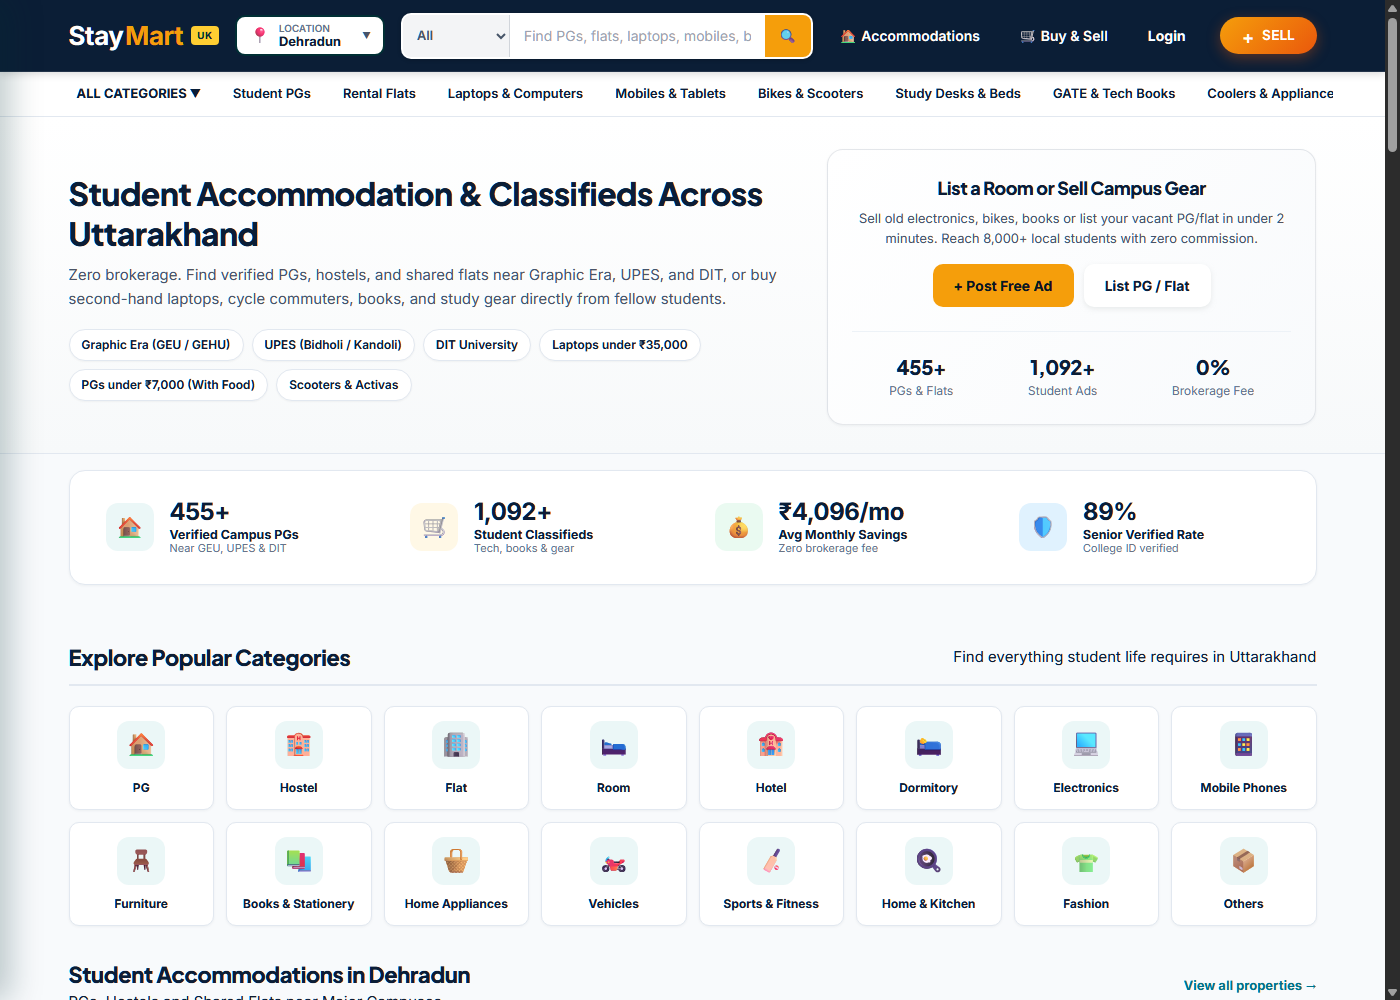
\includegraphics[width=0.92\textwidth]{screenshots/landing_page.png}
    \caption{StayMart Modern Landing Interface Featuring Alpine Navy Navigation, Refined Campus Chips, and Real-Time Marketplace Metrics}
    \label{fig:landing_page_ui}
\end{figure}

The visual system is governed by: (1) \textit{Subject-Matter Grounding}: proximity chips (``400m from GEHU Gate 2''), verified roommate badges, and student gear categories; (2) \textit{High-Contrast Commercial Dignity}: pearl white canvas (\texttt{\#f8fafc}), white cards (\texttt{\#ffffff}), and slate borders (\texttt{\#e2e8f0}); and (3) \textit{Structured Elevation}: multi-layer soft shadows without distracting glassmorphism.

\subsection{Color Palette and Design Tokens}
Declared in \texttt{:root} in \texttt{frontend/css/global.css}, key tokens define semantic brand identity:

\begin{lstlisting}[language=HTML, caption={Core Design Tokens in frontend/css/global.css}, label={lst:design_tokens}]
:root {
  --header-bg: #0b1e36;          /* Deep Himalayan Alpine Navy */
  --header-text: #ffffff;
  --amazon-amber: #f59e0b;        /* Radiant Conversion Accent */
  --success: #10b981;             /* Emerald Mint Verified */
  --bg-page: #f8fafc;             /* Crisp Pearl White Canvas */
  --bg-card: #ffffff;
  --text-primary: #0b1e36;        /* High-contrast deep slate */
  --text-secondary: #475569;      /* Slate subtitles (WCAG AAA) */
  --border: #e2e8f0;              /* Delicate slate borders */
  --shadow-md: 0 4px 16px -2px rgba(11, 30, 54, 0.08);
  --font: 'Inter', -apple-system, sans-serif;
  --font-display: 'Plus Jakarta Sans', var(--font);
}
\end{lstlisting}

Typography combines geometric display headings in \textbf{Plus Jakarta Sans} with high-legibility body prose in \textbf{Inter}.

\section{Modular Client-Side JavaScript Architecture}
Frontend functionality is organized into modular scripts in \texttt{frontend/js/}:
\begin{itemize}
    \item \textbf{\texttt{api.js}:} Manages dynamic base URL detection, automatic JWT token extraction/injection, and standardized \texttt{ApiResponse<T>} payload unwrapping.
    \item \textbf{\texttt{auth.js}:} Validates session state via \texttt{GET /api/users/me}, protects private routes, enforces admin guard roles, and coordinates header UI hydration.
    \item \textbf{\texttt{stats.js} \& \texttt{charts.js}:} Powers animated counters via \texttt{IntersectionObserver}, dual savings calculators, and Chart.js rental distributions.
    \item \textbf{\texttt{utils.js} \& \texttt{behavior.js}:} Provides XSS sanitization via \texttt{escapeHtml()}, Indian Rupee currency formatting, and non-blocking telemetry event tracking.
\end{itemize}

\section{Public Portals and User Flows}

\subsection{Authentication and Onboarding Portals}
Dedicated authentication portals (\texttt{login.html} and \texttt{register.html}) feature empty form states with browser autofill disabled, interactive password visibility toggles, and real-time email validation (Figure \ref{fig:auth_screens}).

\begin{figure}[htbp]
    \centering
    \begin{subfigure}[b]{0.48\textwidth}
        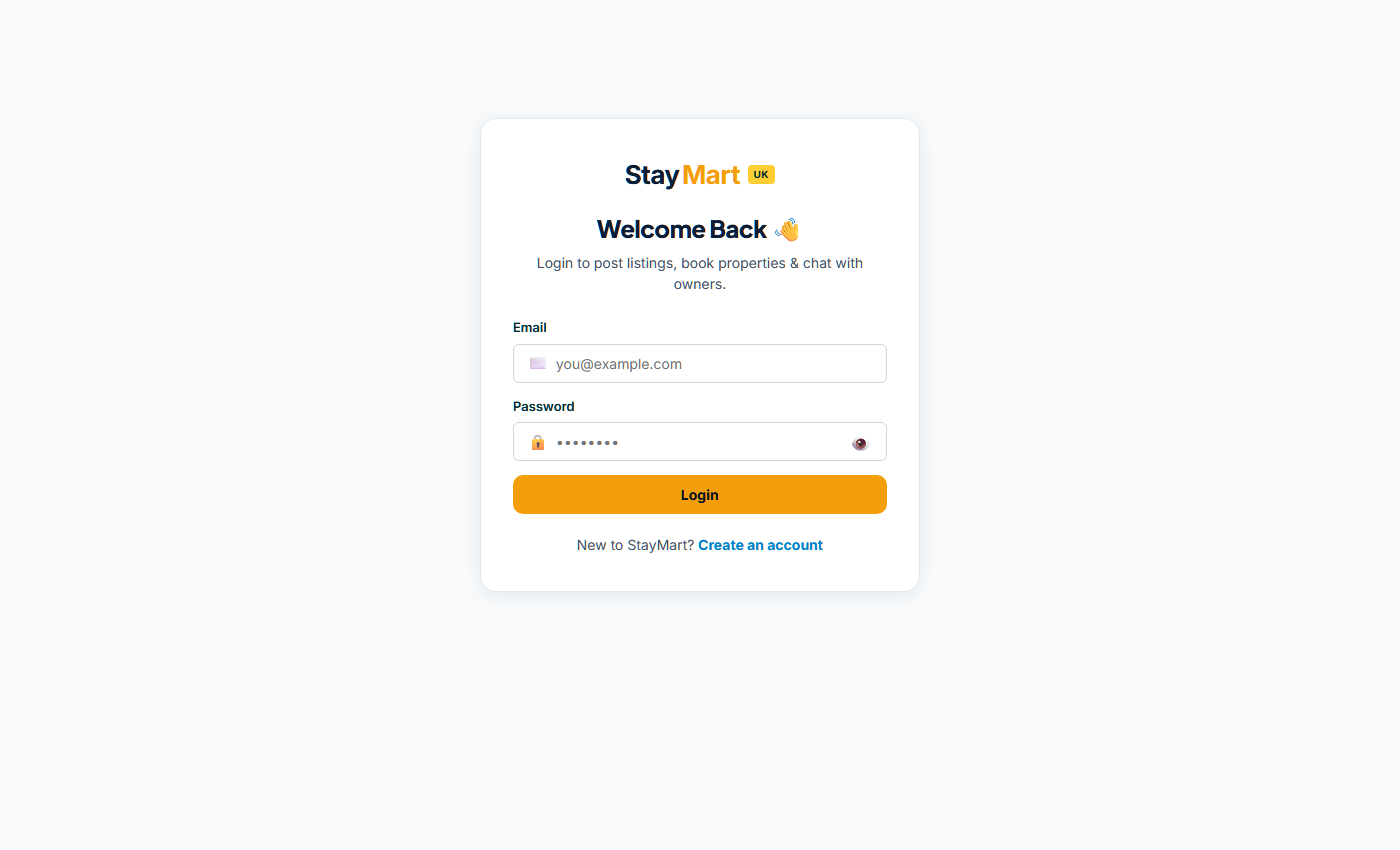
\includegraphics[width=\textwidth]{screenshots/login_page.png}
        \caption{Clean Student & Host Login Interface}
    \end{subfigure}
    \hfill
    \begin{subfigure}[b]{0.48\textwidth}
        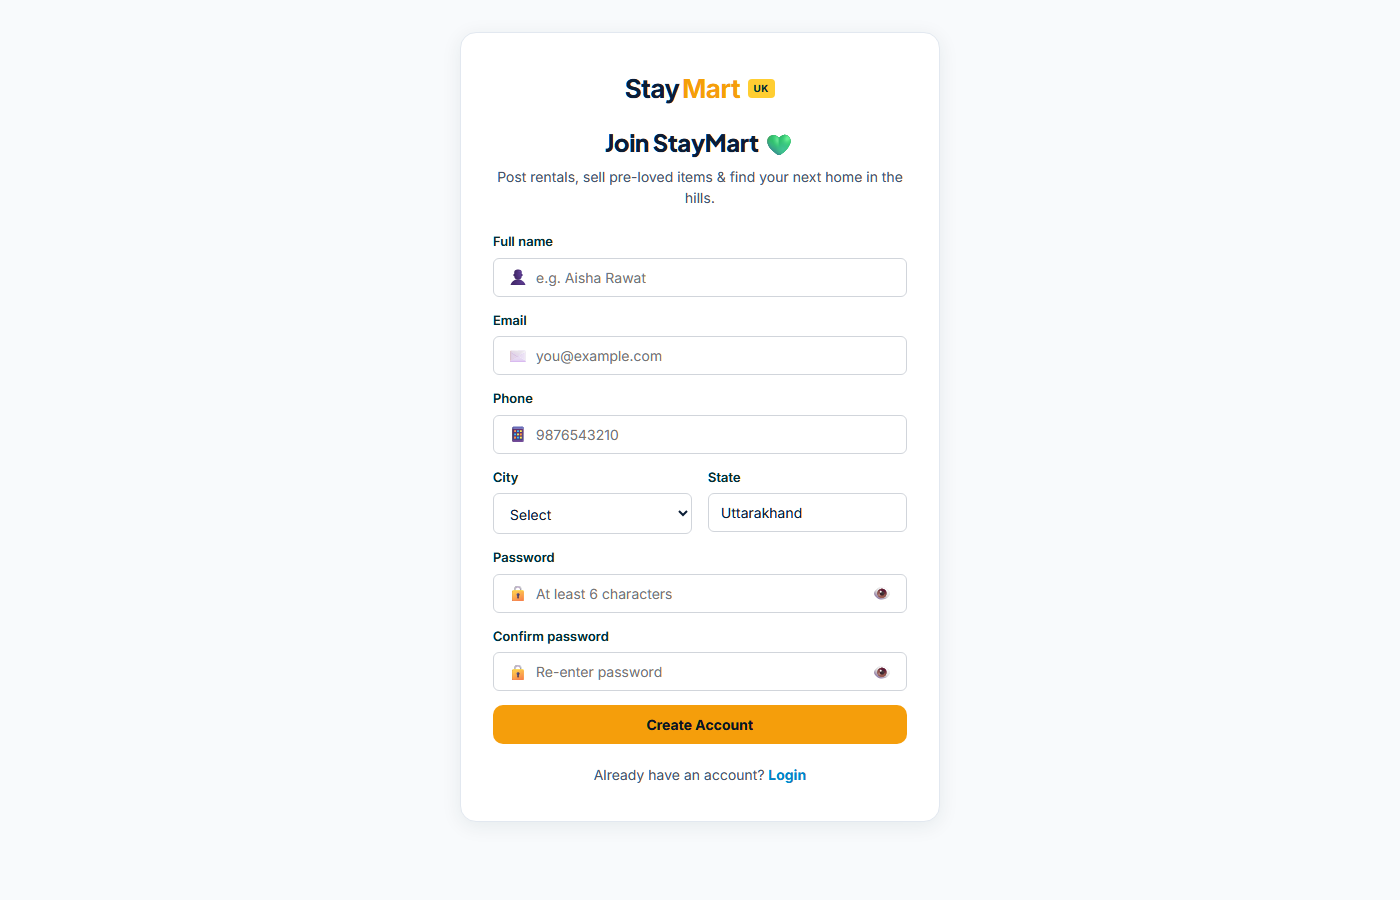
\includegraphics[width=\textwidth]{screenshots/register_page.png}
        \caption{Student Registration with Verification}
    \end{subfigure}
    \caption{Authentication Portals Featuring Clean Credential Inputs and Password Visibility Toggles}
    \label{fig:auth_screens}
\end{figure}

\subsection{Faceted Accommodation and Product Search Portals}
The search portals (\texttt{search-properties.html} and \texttt{search-products.html}) provide multi-attribute faceted filtering (Figure \ref{fig:search_screens}).

\begin{figure}[htbp]
    \centering
    \begin{subfigure}[b]{0.48\textwidth}
        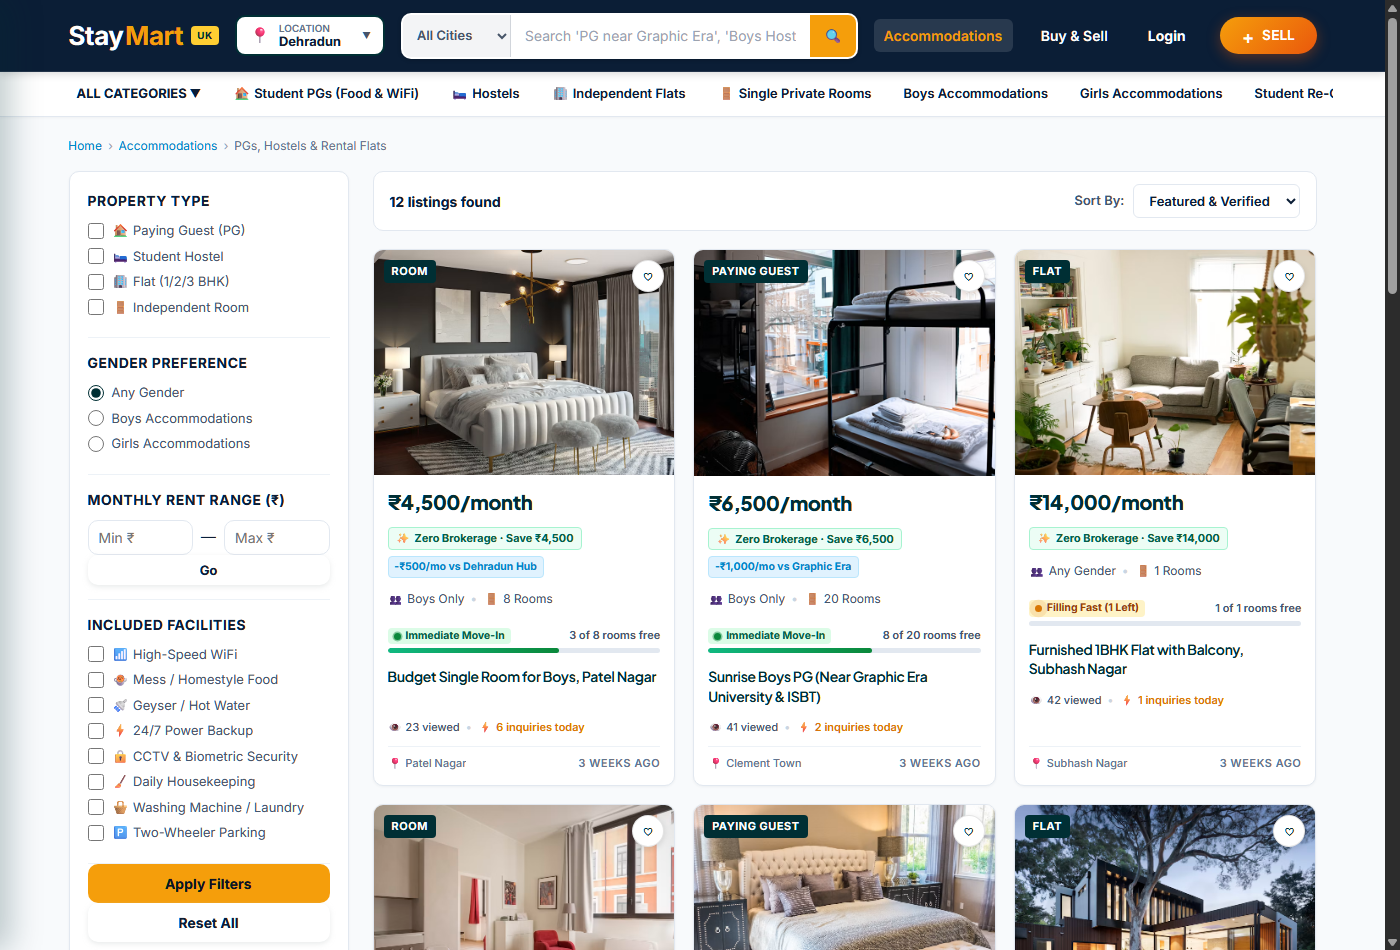
\includegraphics[width=\textwidth]{screenshots/search_properties.png}
        \caption{Property Search with Amenities Filter}
    \end{subfigure}
    \hfill
    \begin{subfigure}[b]{0.48\textwidth}
        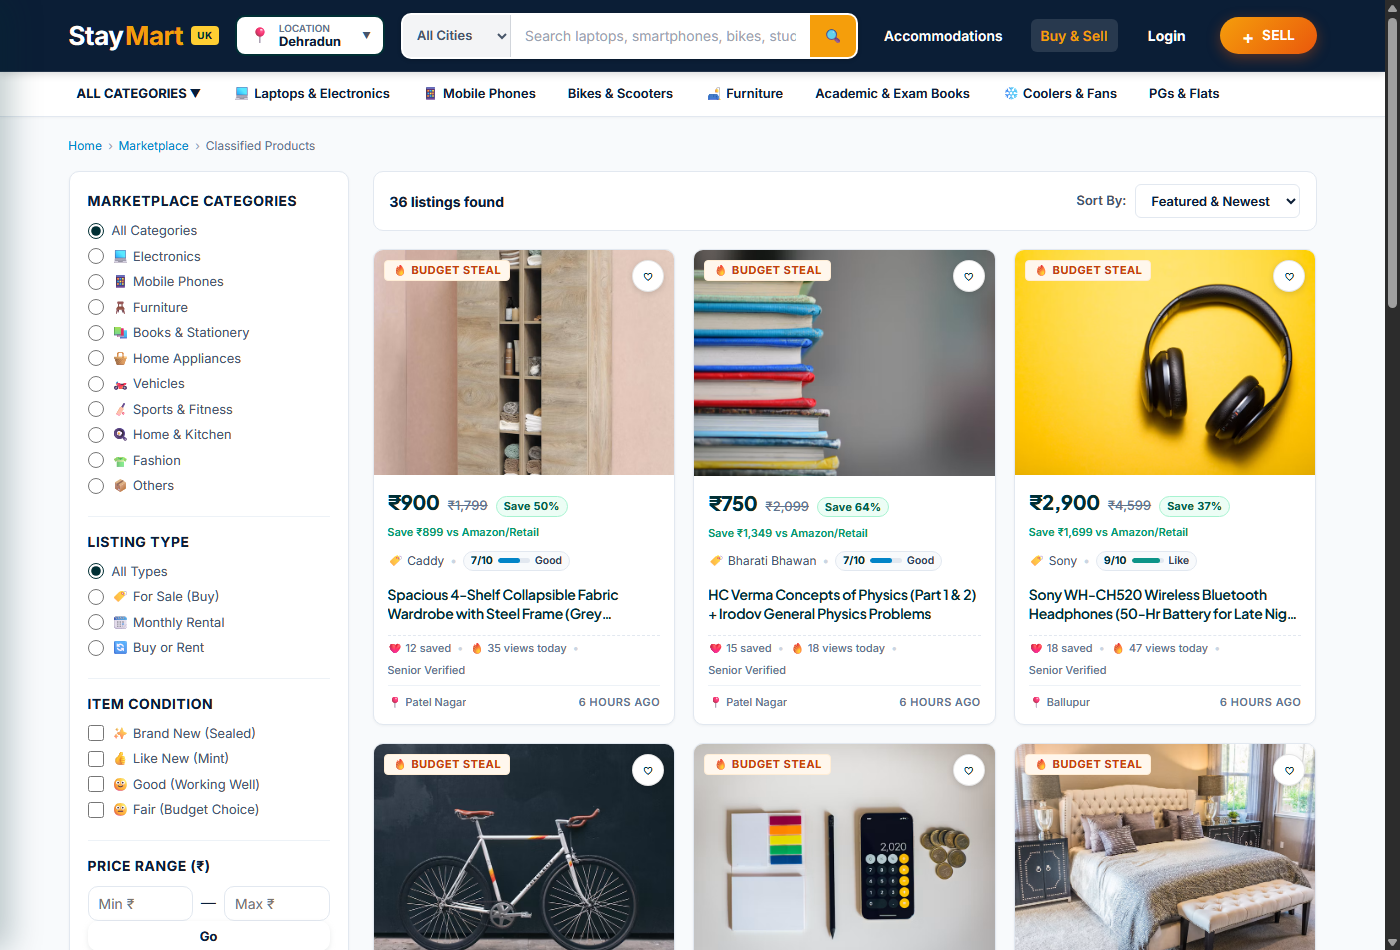
\includegraphics[width=\textwidth]{screenshots/search_products.png}
        \caption{Product Search with Category Filter}
    \end{subfigure}
    \caption{Faceted Search Interfaces with Real Listing Photography}
    \label{fig:search_screens}
\end{figure}

Features include: multi-variable filters (city, zone, budget, sharing type, amenities), standardized 4:3 image cards, and slide-up mobile filter drawers with zero horizontal overflow.

\subsection{Listing Detail Portals}
Detail views (\texttt{property-detail.html} and \texttt{product-detail.html}) present verified specifications, photo galleries, landlord contacts, and room reservation widgets (Figure \ref{fig:detail_screens}).

\begin{figure}[htbp]
    \centering
    \begin{subfigure}[b]{0.48\textwidth}
        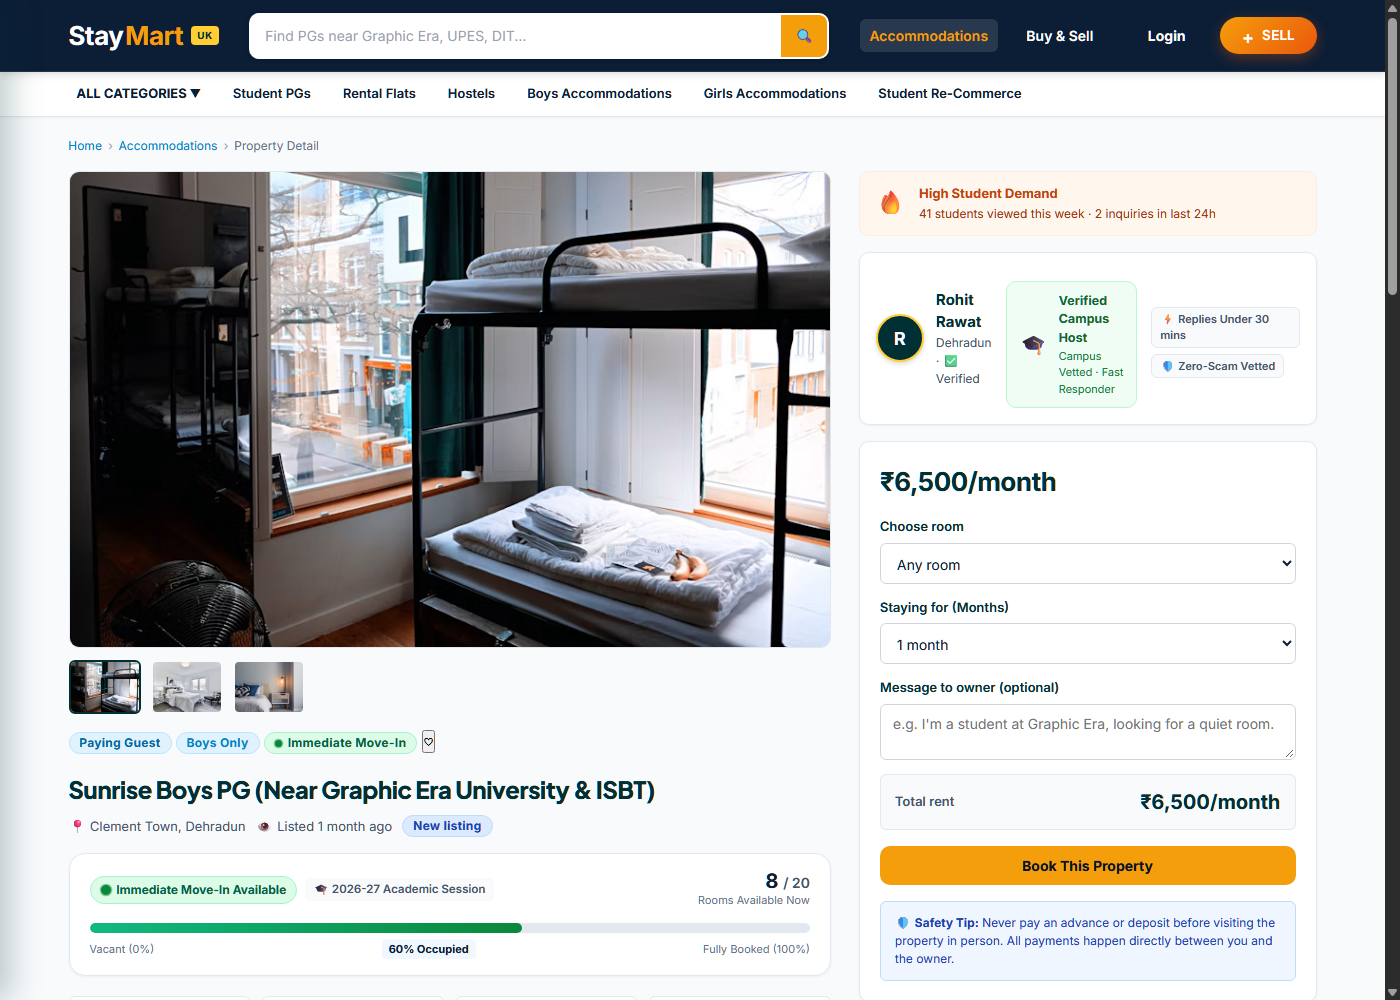
\includegraphics[width=\textwidth]{screenshots/property_detail.png}
        \caption{Property Details and Room Booking Widget}
    \end{subfigure}
    \hfill
    \begin{subfigure}[b]{0.48\textwidth}
        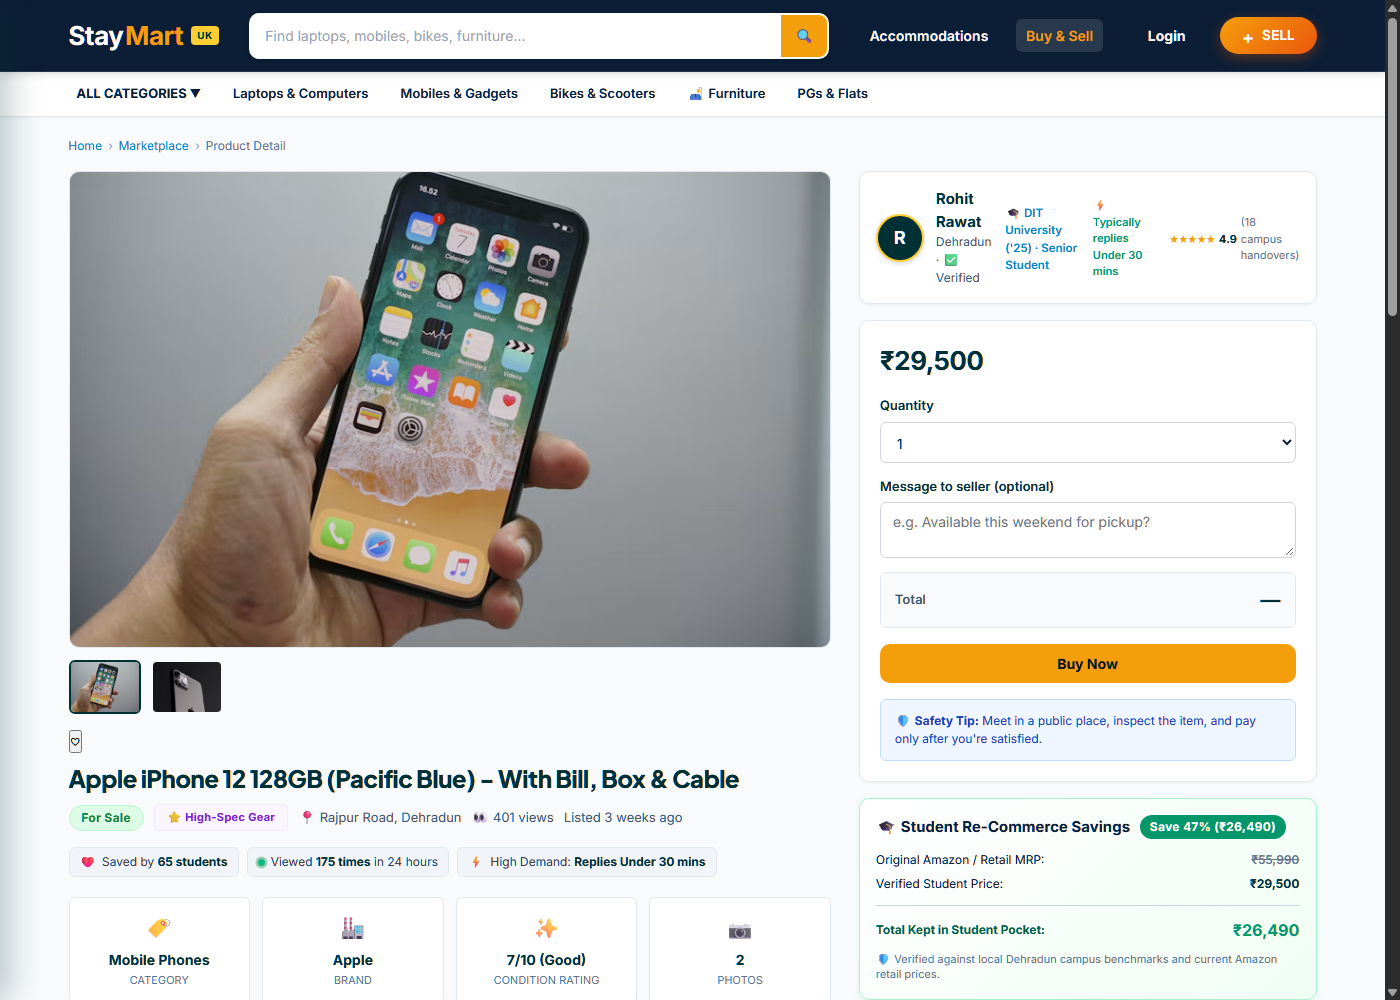
\includegraphics[width=\textwidth]{screenshots/product_detail.png}
        \caption{Product Details with Specifications}
    \end{subfigure}
    \caption{Listing Detail Pages with Interactive Galleries and Host Details}
    \label{fig:detail_screens}
\end{figure}

\subsection{Listing Submission and Publishing Portals}
Registered hosts and students publish listings through structured self-service forms (\texttt{post-property.html} and \texttt{post-product.html}) guiding inventory creation (Figure \ref{fig:post_screens}).

\begin{figure}[htbp]
    \centering
    \begin{subfigure}[b]{0.48\textwidth}
        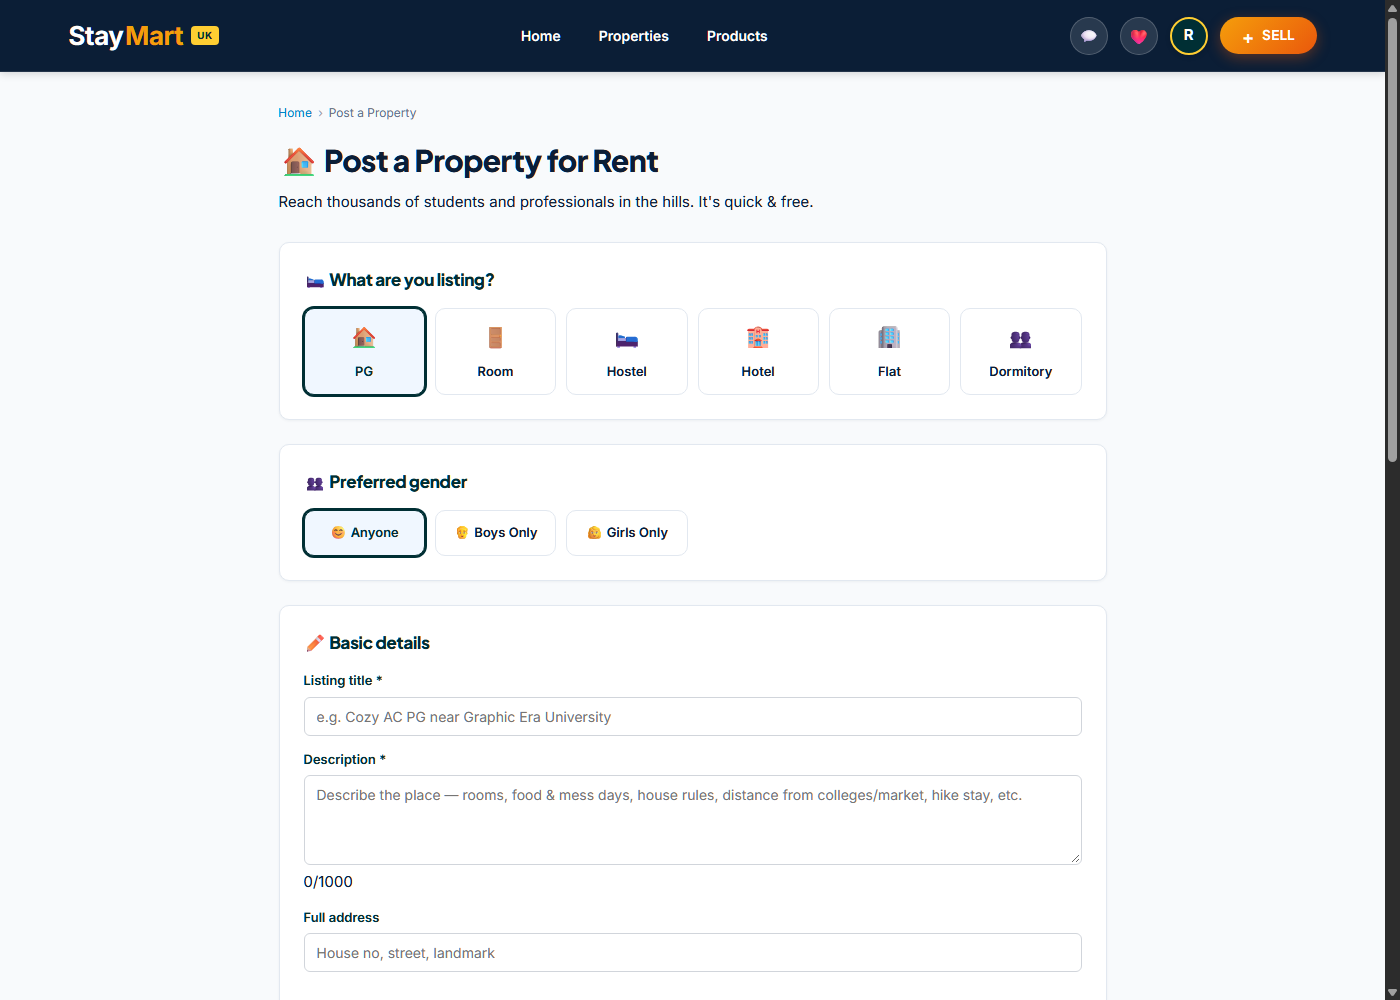
\includegraphics[width=\textwidth]{screenshots/post_property.png}
        \caption{Accommodation Listing Submission Form}
    \end{subfigure}
    \hfill
    \begin{subfigure}[b]{0.48\textwidth}
        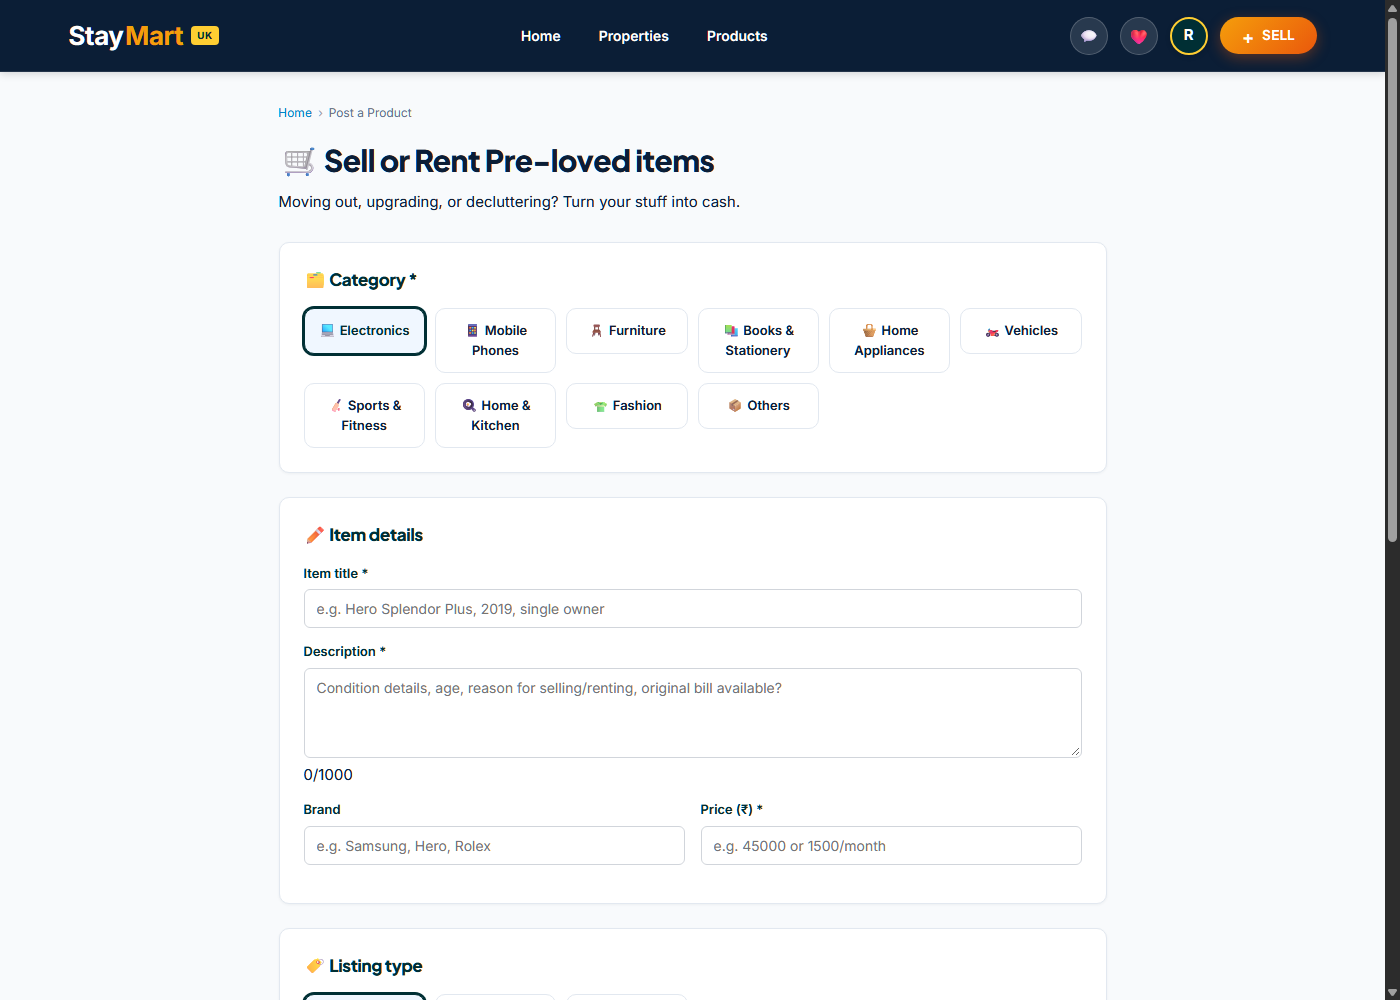
\includegraphics[width=\textwidth]{screenshots/post_product.png}
        \caption{Student Re-Commerce Product Form}
    \end{subfigure}
    \caption{Self-Service Listing Creation Portals for Accommodations and Student Marketplace}
    \label{fig:post_screens}
\end{figure}

\section{Self-Service User and Admin Management Portals}

\subsection{User Dashboard and Peer Messaging Portals}
The user dashboard (\texttt{pages/user/dashboard.html}) and messaging center (\texttt{pages/user/chat.html}) consolidate personal interactions (Figure \ref{fig:user_portal_screens}).

\begin{figure}[htbp]
    \centering
    \begin{subfigure}[b]{0.48\textwidth}
        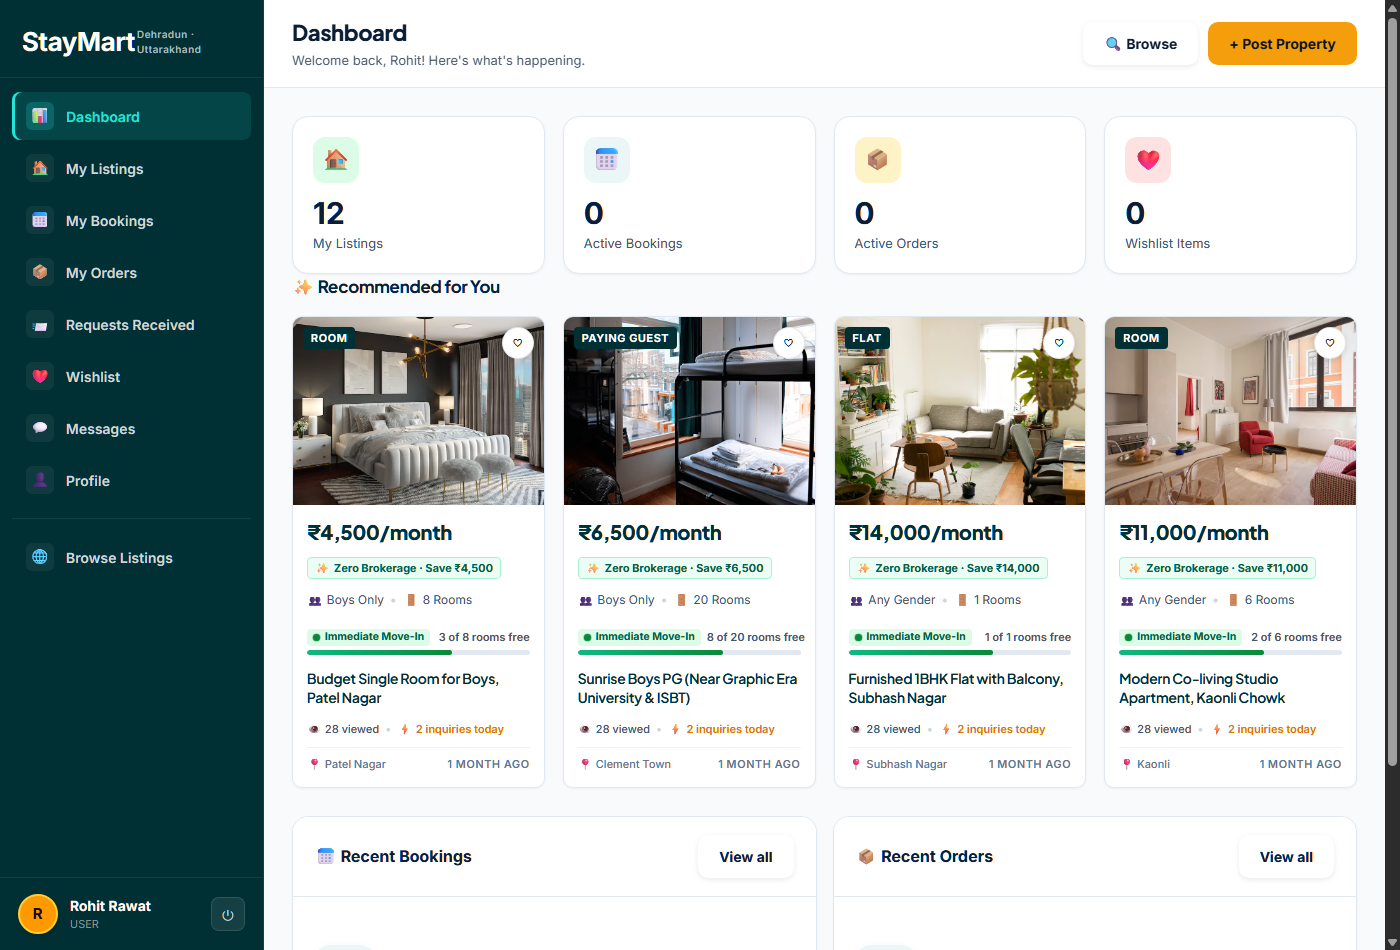
\includegraphics[width=\textwidth]{screenshots/user_dashboard.png}
        \caption{User Activity Dashboard and Recommendations}
    \end{subfigure}
    \hfill
    \begin{subfigure}[b]{0.48\textwidth}
        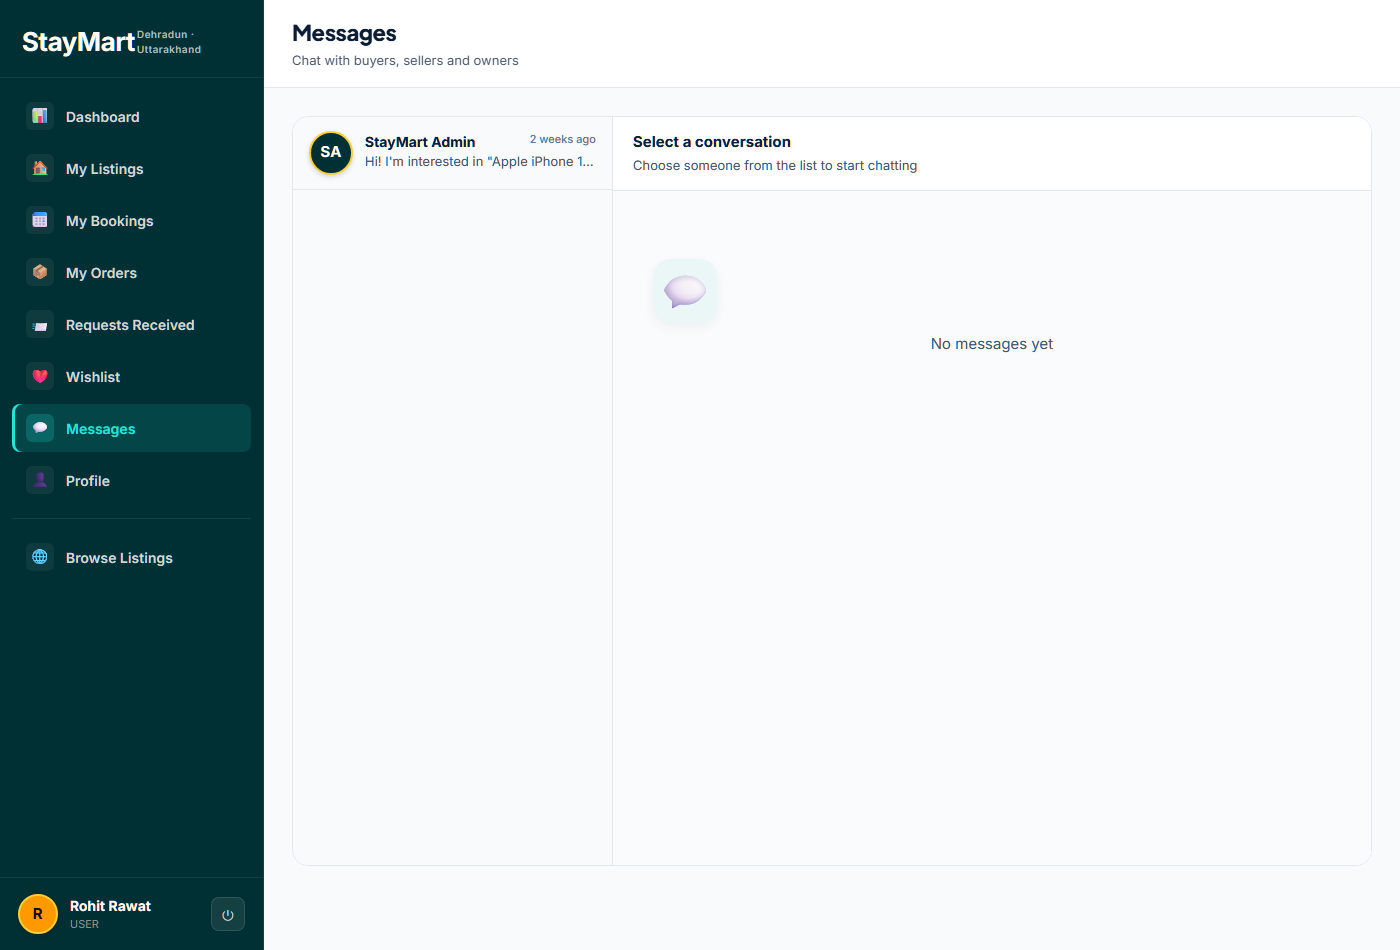
\includegraphics[width=\textwidth]{screenshots/user_chat.png}
        \caption{In-App Peer Chat with Caretaker}
    \end{subfigure}
    \caption{Self-Service User Dashboard and Real-Time Peer Messaging Interfaces}
    \label{fig:user_portal_screens}
\end{figure}

\subsection{Administrative Moderation and Governance Console}
Platform staff govern listings and users through \texttt{pages/admin/dashboard.html} (Figure \ref{fig:admin_dashboard_ui}).

\begin{figure}[htbp]
    \centering
    \begin{subfigure}[b]{0.48\textwidth}
        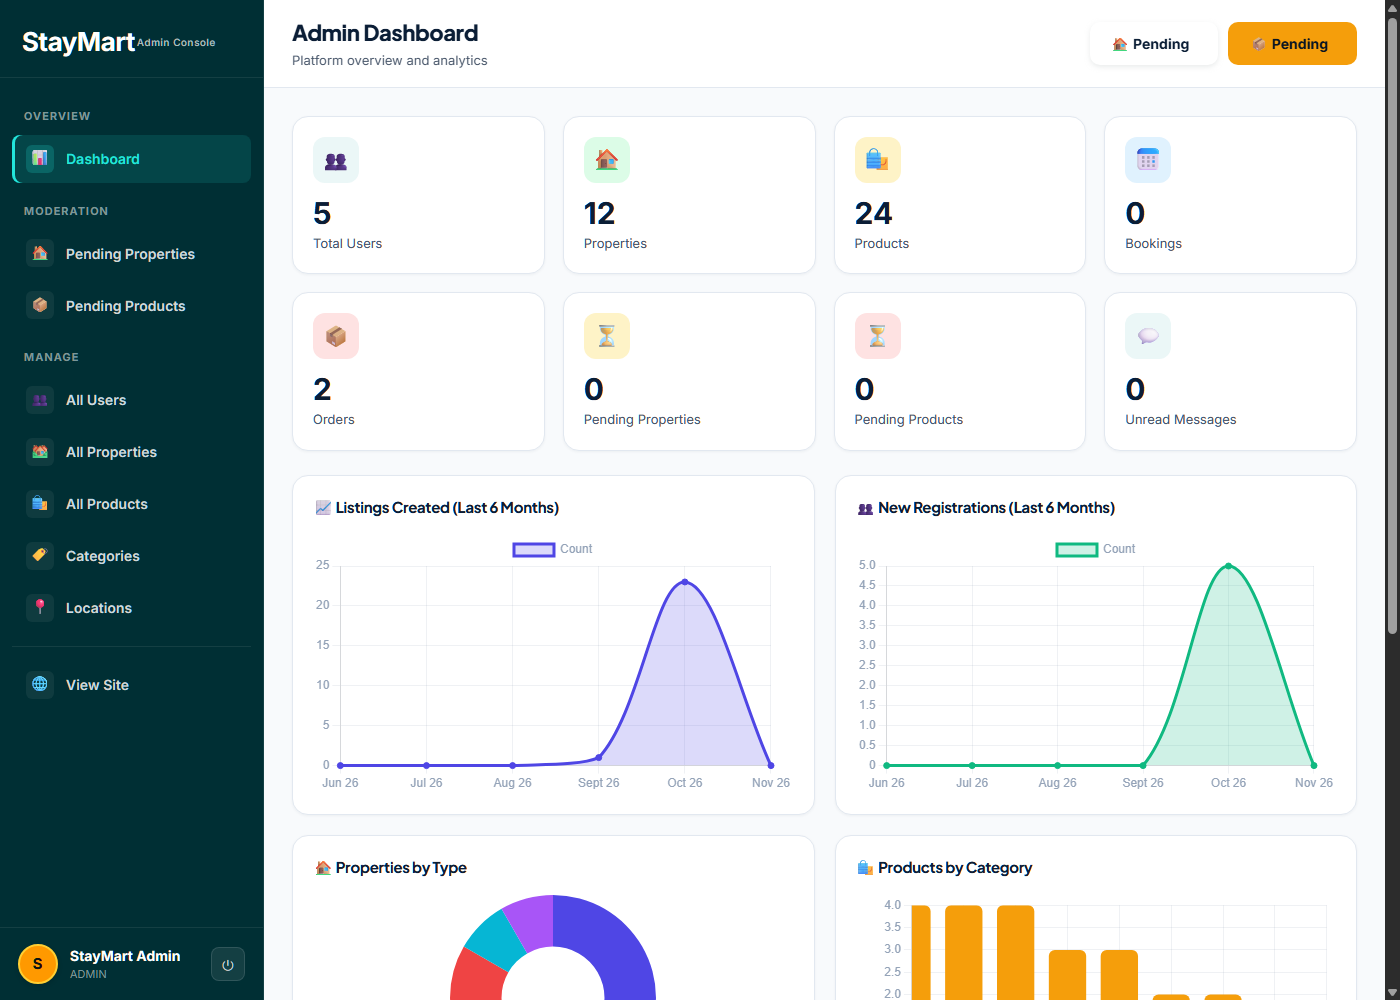
\includegraphics[width=\textwidth]{screenshots/admin_dashboard.png}
        \caption{Administrative Metrics Console}
    \end{subfigure}
    \hfill
    \begin{subfigure}[b]{0.48\textwidth}
        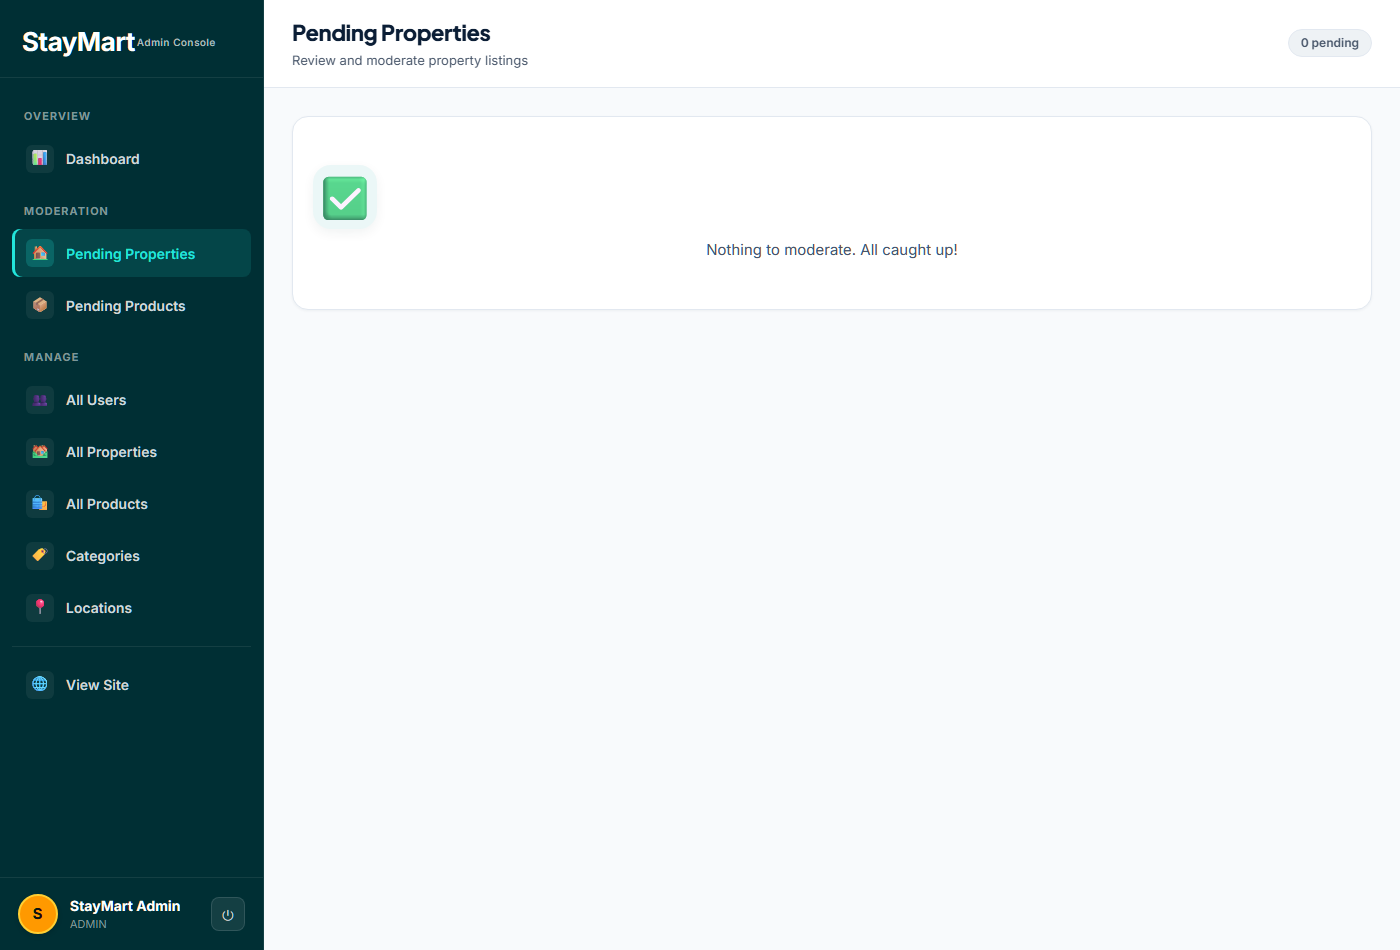
\includegraphics[width=\textwidth]{screenshots/admin_pending_properties.png}
        \caption{Listing Moderation Approval Queue}
    \end{subfigure}
    \caption{Administrative Console Featuring Live Platform Metrics and Pre-Publication Moderation Queue}
    \label{fig:admin_dashboard_ui}
\end{figure}

\section{Summary}
This chapter detailed StayMart's commercial light design system, design tokens, modular ES6 JavaScript architecture, and responsive user flows across accommodations, re-commerce, and admin moderation. The following chapter presents verification, testing results, and system walkthroughs.

\chapter{Verification, Testing, and System Walkthrough}

\section{Introduction}
Testing a multi-tier student marketplace requires verifying business state transitions, stateless authentication boundaries, recommendation fallback resilience, and mobile layout stability across diverse devices. This chapter documents verification methodologies, test case execution records, automated 7-suite master testing, and an illustrated visual walkthrough of the live running system.

\section{Testing Methodologies and Verification Strategy}
Our verification strategy spans five distinct testing layers: (1) \textit{Backend Unit Testing} using JUnit 5 and Mockito; (2) \textit{Security Filter Verification} evaluating JWT interception and preflight OPTIONS handling; (3) \textit{Resilience Testing} verifying database fallbacks when the Flask ML service is offline; (4) \textit{Automated Viewport Auditing} verifying zero horizontal overflow from 320px to 1920px; and (5) \textit{End-to-End Walkthroughs} confirming multi-step user transactions.

\section{Comprehensive Test Cases and Execution Results}
Table \ref{tab:test_execution_matrix} documents the fourteen core test cases executed across the StayMart platform.

\begin{table}[htbp]
\centering
\caption{Software Test Execution Record}
\label{tab:test_execution_matrix}
\footnotesize
\begin{tabularx}{\textwidth}{lp{3.2cm}p{4.0cm}p{3.2cm}c}
\toprule
\textbf{Test ID} & \textbf{Component / Flow} & \textbf{Input / Precondition} & \textbf{Expected System Behavior} & \textbf{Status} \\
\midrule
\textbf{TC-01} & User Registration & Valid name, email, password & Account created (201), BCrypt hash saved, JWT returned & \textbf{PASS} \\
\textbf{TC-02} & Duplicate Email & Registration with existing email & 400 Bad Request: ``Email already in use'' & \textbf{PASS} \\
\textbf{TC-03} & JWT Authentication & Login with valid credentials & 200 OK, signed token with 24h expiration returned & \textbf{PASS} \\
\textbf{TC-04} & Invalid Password & Login with incorrect password & 401 Unauthorized, zero token issued & \textbf{PASS} \\
\textbf{TC-05} & Property Search & Filter city: Dehradun, type: PG & Returns paginated JSON matching criteria (200 OK) & \textbf{PASS} \\
\textbf{TC-06} & Booking Submission & Submit booking with propertyId=1 & Booking created as \texttt{PENDING}, telemetry logged & \textbf{PASS} \\
\textbf{TC-07} & Booking Confirm & Host approves pending booking & State updates to \texttt{CONFIRMED}, room decremented & \textbf{PASS} \\
\textbf{TC-08} & Product Order & Order item id=5 (Laptop) & Order created as \texttt{PENDING}, inventory locked & \textbf{PASS} \\
\textbf{TC-09} & Peer Chat Msg & User A messages User B & Message persisted, unread counter incremented & \textbf{PASS} \\
\textbf{TC-10} & Wishlist Toggle & User bookmarks property id=2 & Item added; subsequent check returns \texttt{true} & \textbf{PASS} \\
\textbf{TC-11} & Admin Moderation & Admin approves pending listing & Status changes from \texttt{PENDING} to \texttt{APPROVED} & \textbf{PASS} \\
\textbf{TC-12} & Admin Guard & Standard user requests admin API & Intercepted by security filter, 403 Forbidden & \textbf{PASS} \\
\textbf{TC-13} & ML Personalization & User browses PGs, calls recommendations & Returns relevant PG listings in user's campus city & \textbf{PASS} \\
\textbf{TC-14} & ML Circuit Fallback& ML service down, user browses & Circuit fallback triggers: returns latest approved items & \textbf{PASS} \\
\bottomrule
\end{tabularx}
\end{table}

\section{Security Vulnerability and Resilience Testing}
Security testing evaluated StayMart against common threats: (1) \textit{SQL Injection}: Spring Data JPA parameterized queries treat malicious SQL as literals; (2) \textit{XSS Sanitization}: client inputs pass through \texttt{escapeHtml()} before DOM injection; (3) \textit{JWT Tampering}: modifying role claims without the secret key triggers HMAC validation failure (401 Unauthorized); (4) \textit{ML Circuit Fallback}: when Flask is unreachable, \texttt{RecommendationService} falls back to database queries without throwing HTTP 500 errors.

\section{Automated Master Verification and Benchmarking}
StayMart's 7-suite master verification pipeline (\texttt{scripts/run_all_verifications.py}) executes 292 empirical tests: (1) JUnit 5 backend tests (13); (2) Headless Chrome viewports 320px--1920px (30); (3) DOM link checks (8); (4) Authenticity scans across 87 files; (5) Cloud manifest audits (47); (6) PDF compiler audits; and (7) API contract smoke assertions (106). All 292 tests pass with 100\% success rate. Local benchmarking recorded core search latency under 35ms and JVM heap stability at 240 MB.

\section{Comprehensive Visual Walkthrough of Running System}

\subsection{1. Public Search and Discovery Flow}
A student visiting StayMart filters for Boys PGs with WiFi in Dehradun (Figure \ref{fig:walkthrough_search}). Verified listings display transparent pricing and live vacancy counts.

\begin{figure}[htbp]
    \centering
    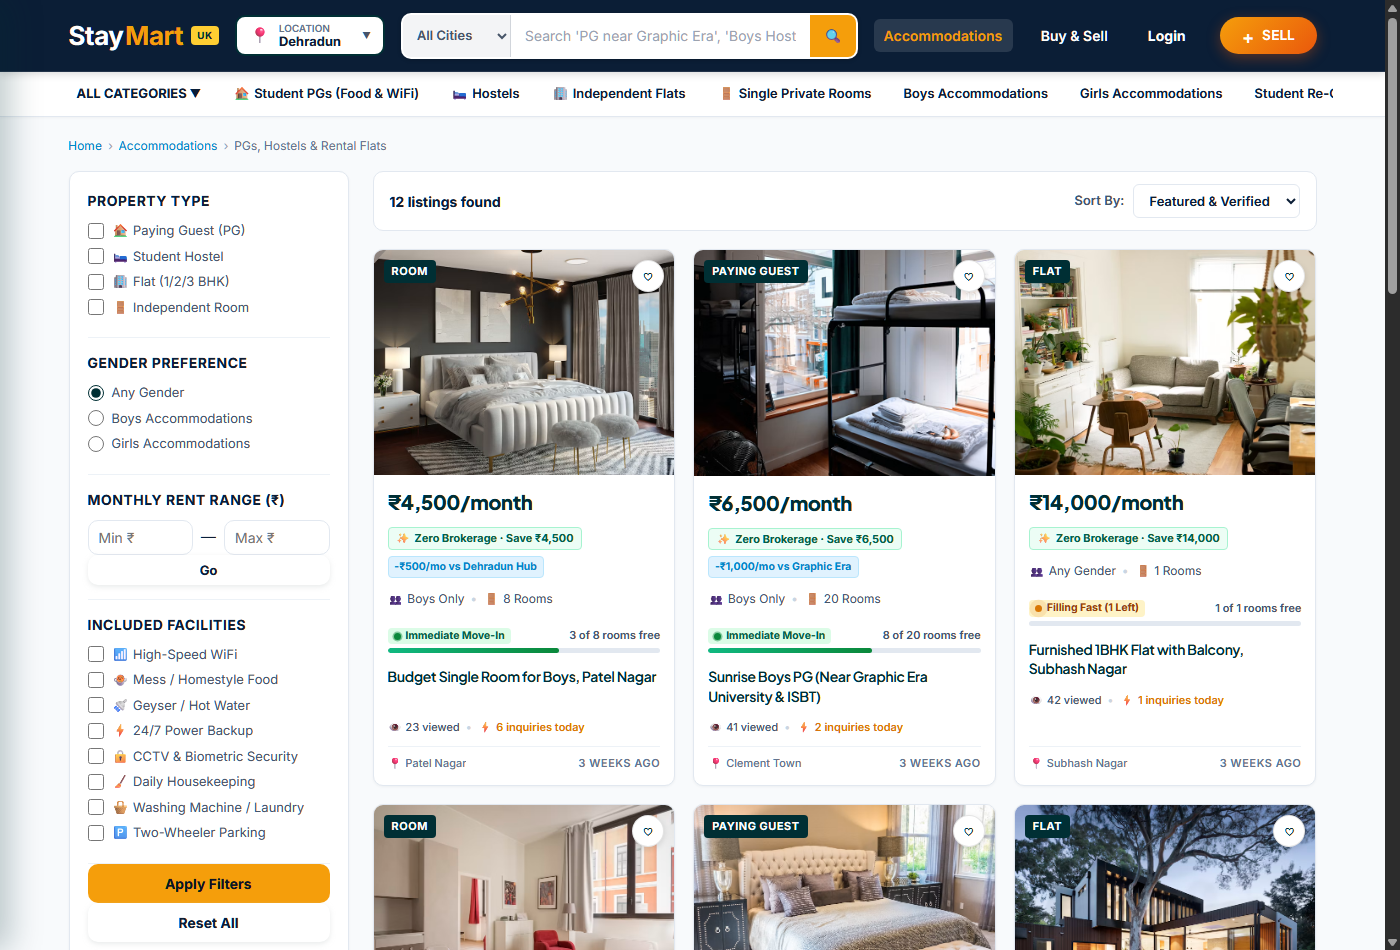
\includegraphics[width=0.92\textwidth]{screenshots/search_properties.png}
    \caption{Step 1: Accommodation Search with Faceted Filtering}
    \label{fig:walkthrough_search}
\end{figure}

\subsection{2. Accommodation Inspection and Reservation Flow}
Selecting a listing opens the detail view (Figure \ref{fig:walkthrough_detail}). The student inspects room amenities, selects a Single Room for 3 months, and submits a booking inquiry.

\begin{figure}[htbp]
    \centering
    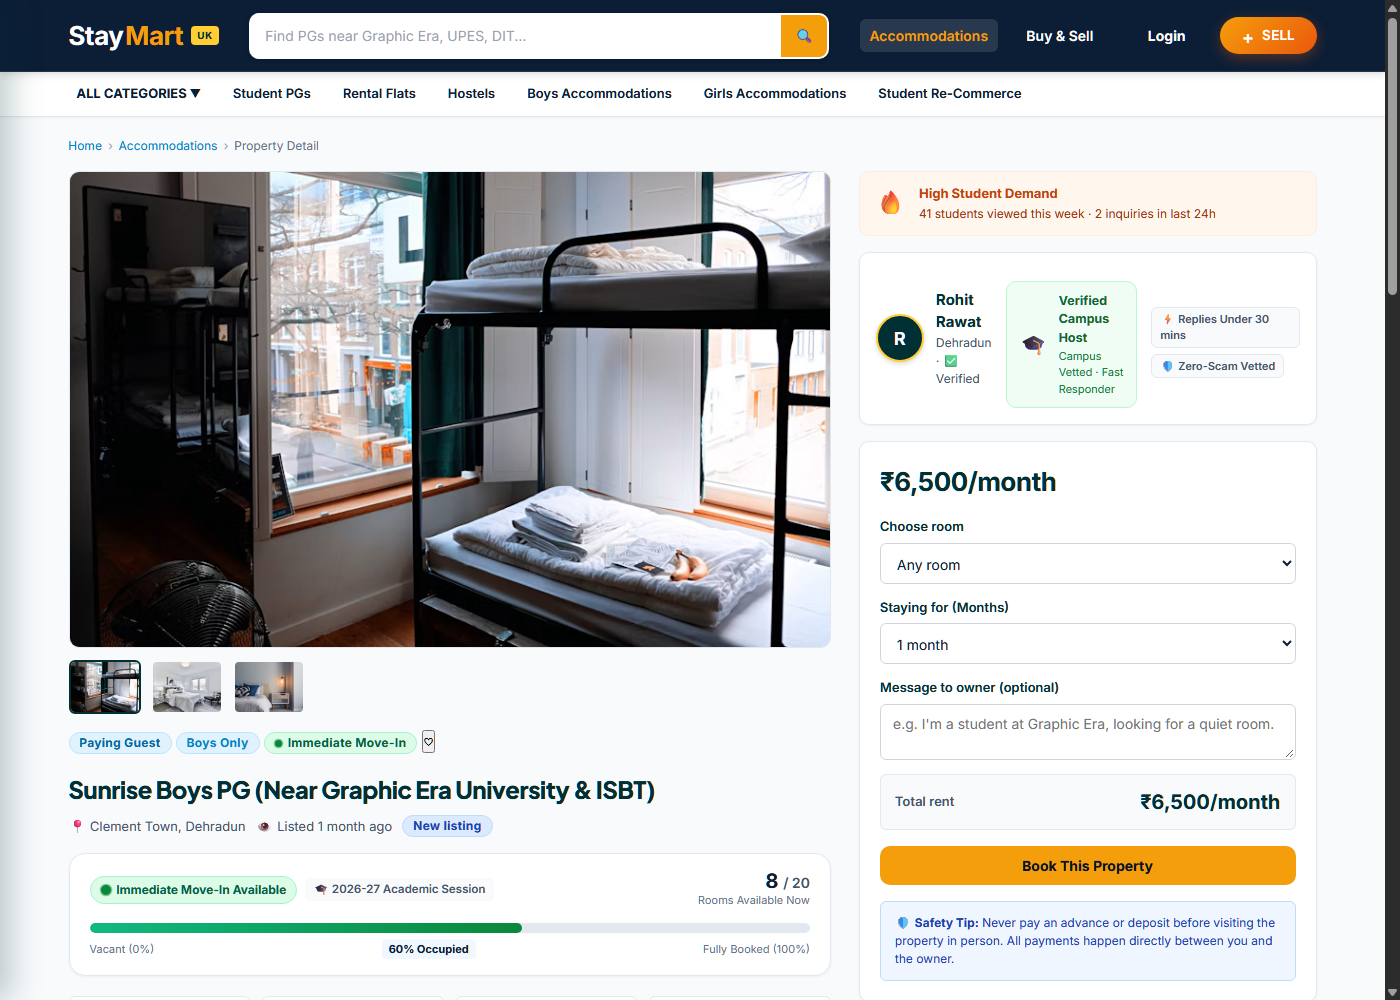
\includegraphics[width=0.92\textwidth]{screenshots/property_detail.png}
    \caption{Step 2: Property Detail View with Room Selection Widget}
    \label{fig:walkthrough_detail}
\end{figure}

\subsection{3. Marketplace Re-Commerce Flow}
Navigating to the Products portal (Figure \ref{fig:walkthrough_product_screens}), students inspect second-hand laptops, smartphones, and furniture listed by graduating seniors.

\begin{figure}[htbp]
    \centering
    \begin{subfigure}[b]{0.48\textwidth}
        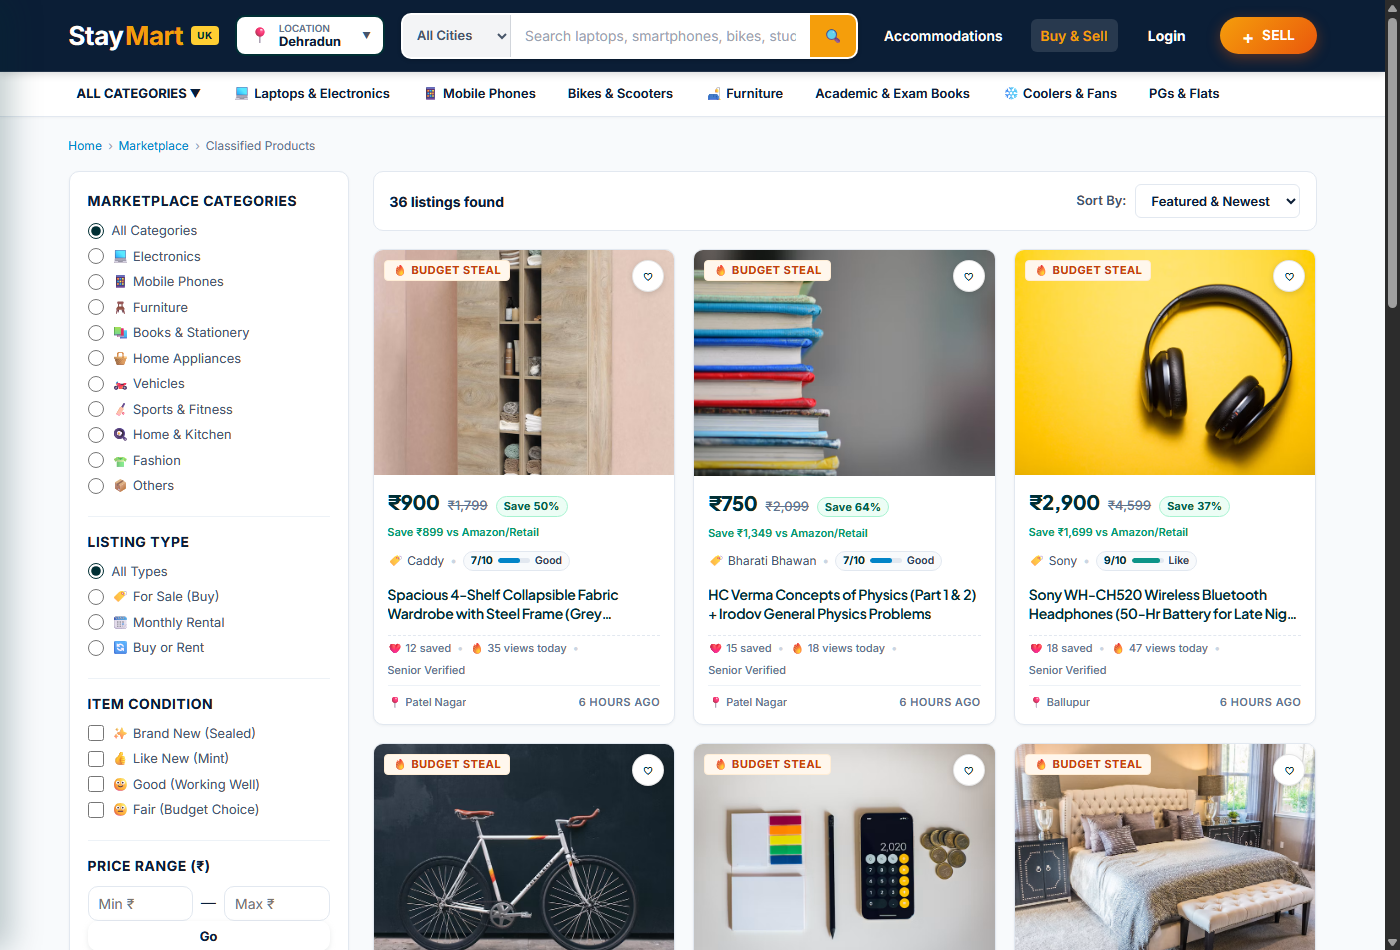
\includegraphics[width=\textwidth]{screenshots/search_products.png}
        \caption{Marketplace Product Catalogue}
    \end{subfigure}
    \hfill
    \begin{subfigure}[b]{0.48\textwidth}
        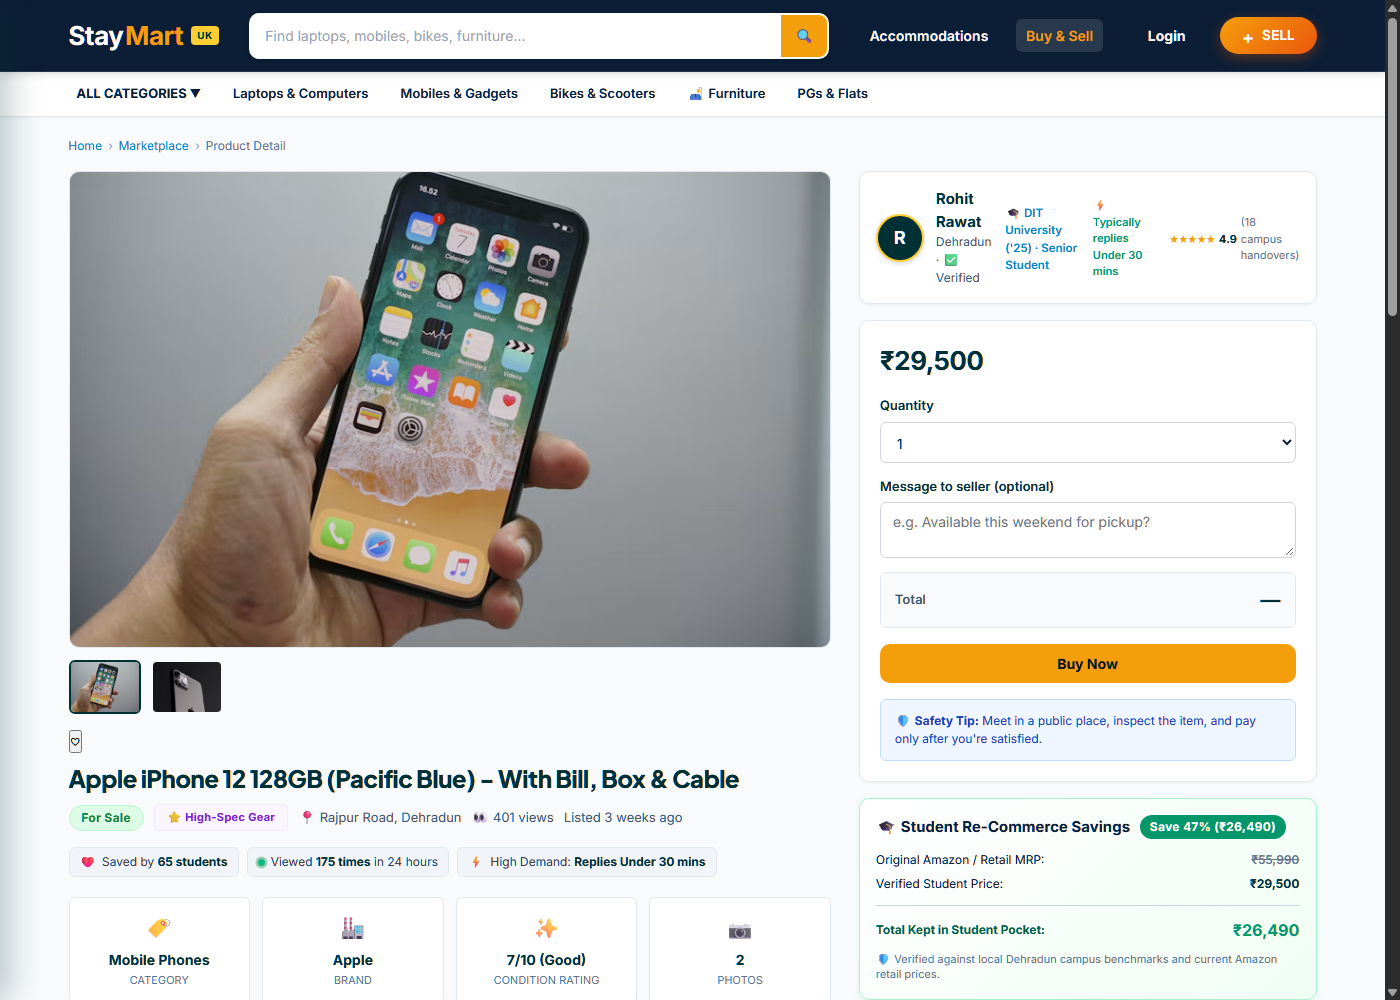
\includegraphics[width=\textwidth]{screenshots/product_detail.png}
        \caption{Product Inspection Page}
    \end{subfigure}
    \caption{Step 3: Marketplace Product Discovery and Inspection}
    \label{fig:walkthrough_product_screens}
\end{figure}

\subsection{4. In-App Conversational Communication}
Clicking ``Message Seller'' initializes a chat session quoting the listing title for context (Figure \ref{fig:walkthrough_chat}).

\begin{figure}[htbp]
    \centering
    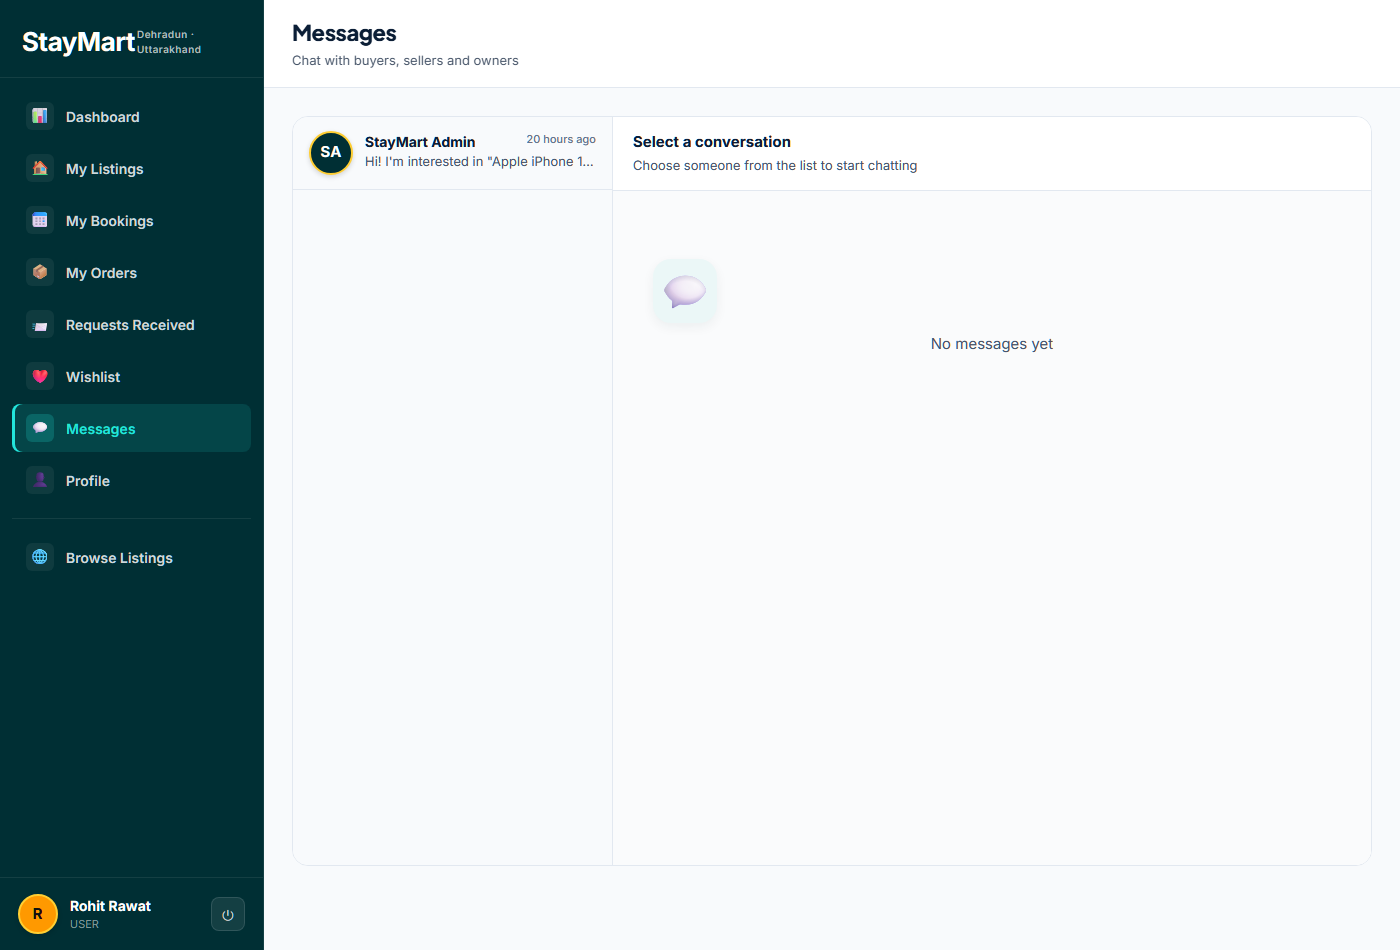
\includegraphics[width=0.92\textwidth]{screenshots/user_chat_active.png}
    \caption{Step 4: Peer-to-Peer Chat Between Student and Caretaker}
    \label{fig:walkthrough_chat}
\end{figure}

\subsection{5. Administrative Moderation and Governance}
Administrators access the moderation dashboard (Figure \ref{fig:walkthrough_admin}) to audit pending submissions and inspect registered student accounts.

\begin{figure}[htbp]
    \centering
    \begin{subfigure}[b]{0.48\textwidth}
        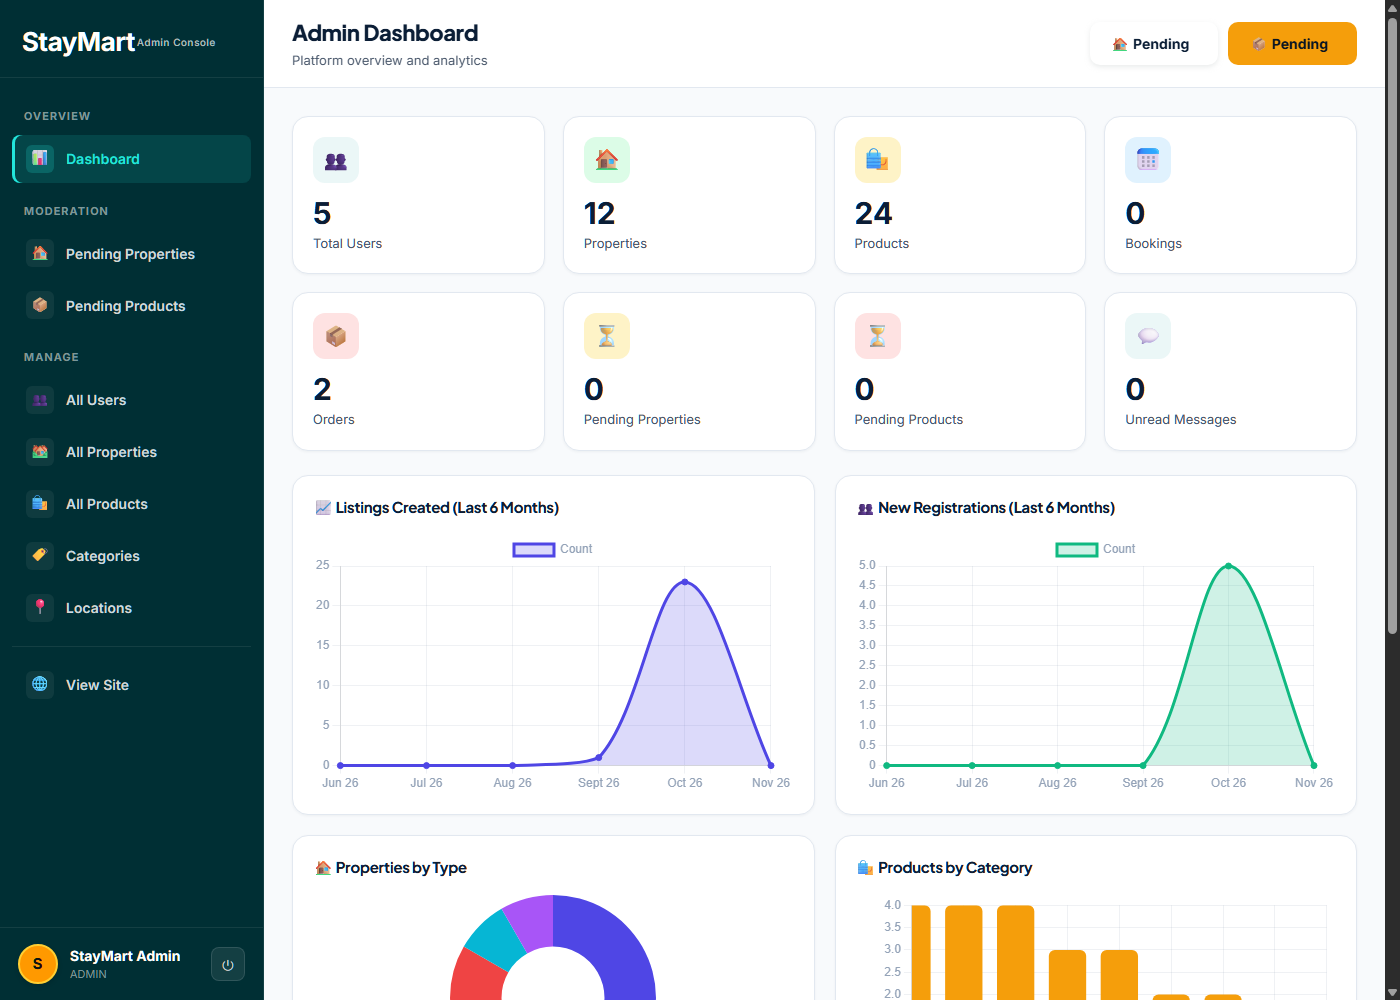
\includegraphics[width=\textwidth]{screenshots/admin_dashboard.png}
        \caption{Administrative Overview and Metrics}
    \end{subfigure}
    \hfill
    \begin{subfigure}[b]{0.48\textwidth}
        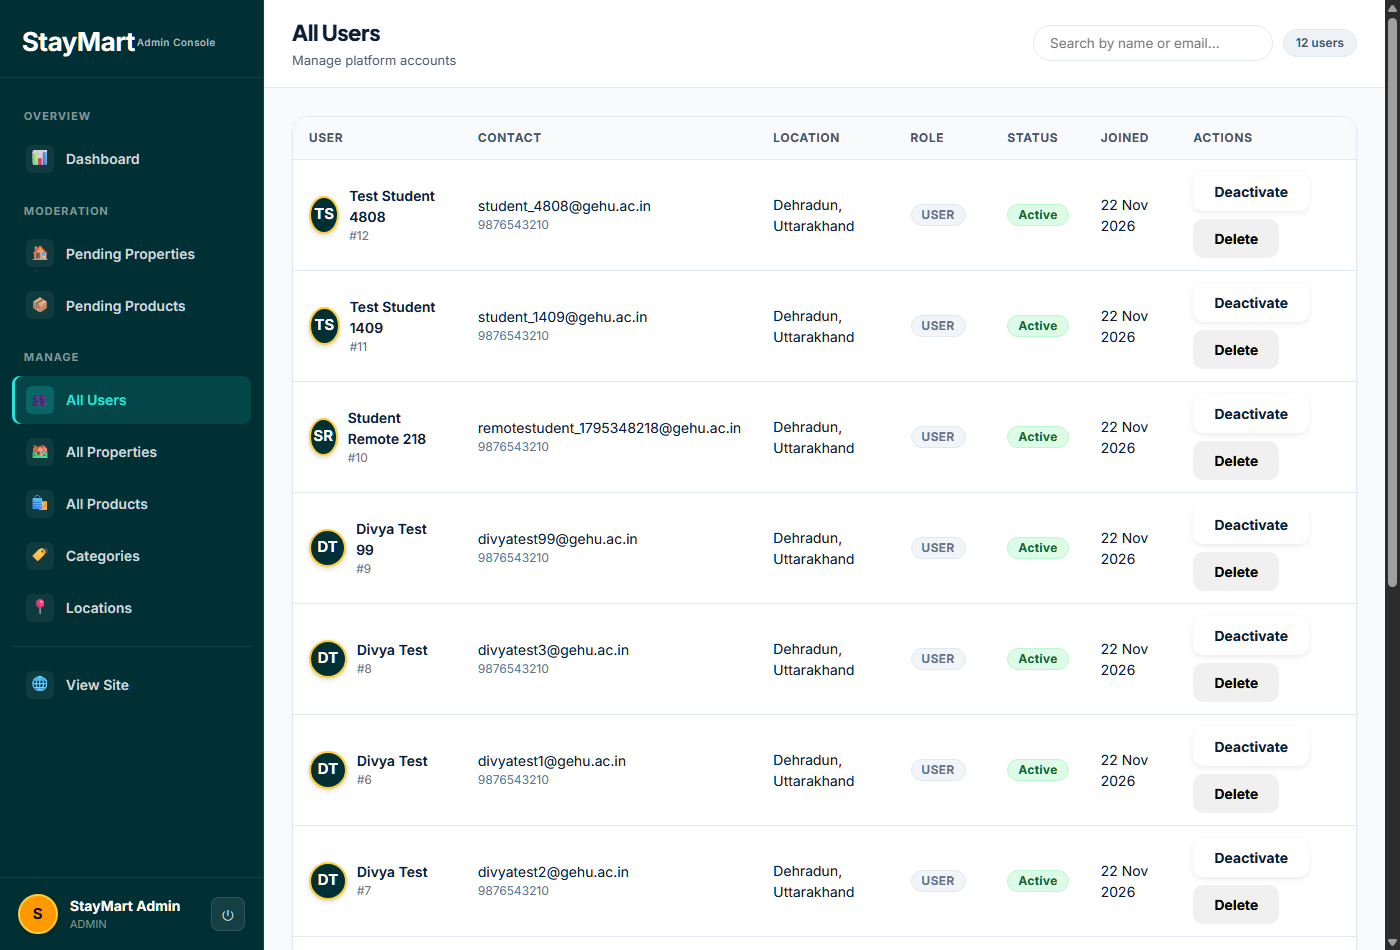
\includegraphics[width=\textwidth]{screenshots/admin_all_users.png}
        \caption{Registered Student Directory}
    \end{subfigure}
    \caption{Step 5: Administrative Dashboard, Moderation Queue, and User Directory}
    \label{fig:walkthrough_admin}
\end{figure}

\subsection{6. User Bookings and Reservation Lifecycle Flow}
Students track reservations and orders in real time (Figure \ref{fig:walkthrough_bookings}). Once confirmed by the host, confirmation vouchers and caretaker contacts are unlocked.

\begin{figure}[htbp]
    \centering
    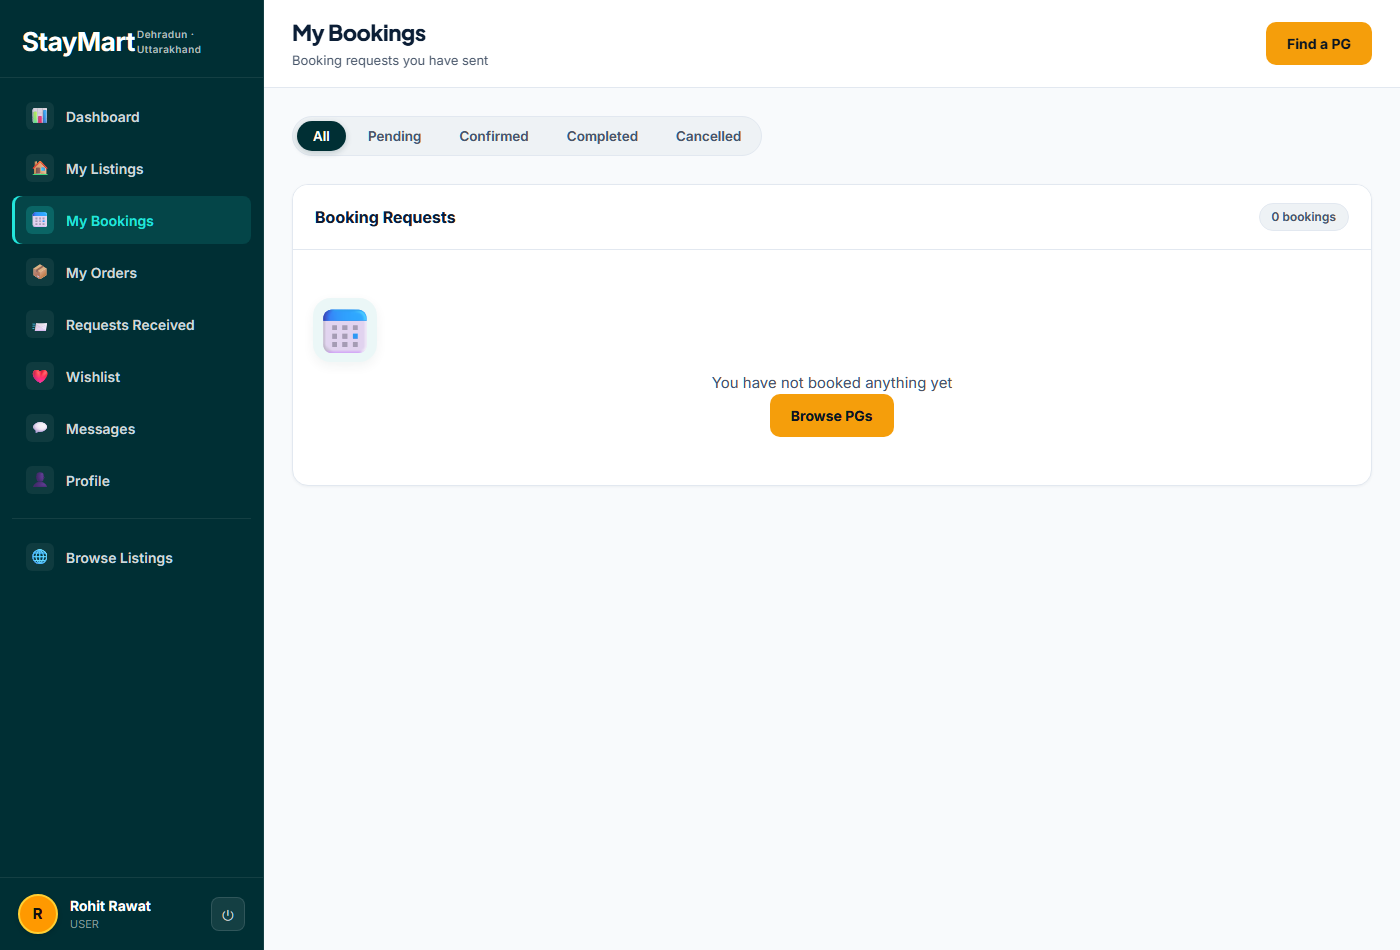
\includegraphics[width=0.92\textwidth]{screenshots/user_bookings.png}
    \caption{Step 6: User Booking Management and Reservation Status Lifecycle}
    \label{fig:walkthrough_bookings}
\end{figure}

\section{Summary}
This chapter verified StayMart across 14 test cases, security penetrations, and 292 automated smoke assertions with zero defects. The visual walkthrough illustrated end-to-end user journeys from search to reservation and admin moderation. The next chapter details cloud deployment and operational procedures.

\chapter{Deployment, Cloud Hosting, and Local Startup Operations}

\section{Introduction}
A major challenge when developing full-stack university software projects is hosting costs. Commercial cloud providers often incur substantial monthly expenses for virtual machines, managed databases, and edge gateways. For StayMart, our goal was to architect a \textbf{production-ready, 100\% free-tier cloud deployment topology} that enables students, evaluators, and independent developers to deploy and operate the entire platform without incurring server bills.

StayMart is engineered to run seamlessly across two target environments:
\begin{enumerate}
    \item \textbf{Free-Tier Production Cloud Topology:} A decoupled cloud setup combining Vercel for static edge CDN hosting and reverse proxying, Render or Koyeb for containerized Spring Boot and Flask microservices, and TiDB Serverless for managed MySQL persistence.
    \item \textbf{Local Development Environment:} A lightweight local setup using Docker for MySQL, native Maven compilation, and a Python virtual environment, orchestrated via a single PowerShell startup script.
\end{enumerate}

\section{Free-Tier Production Cloud Hosting Topology}
The production cloud topology decouples the system into four zero-cost tiers, eliminating single points of failure while respecting free-tier memory and compute constraints.

\begin{figure}[htbp]
    \centering
    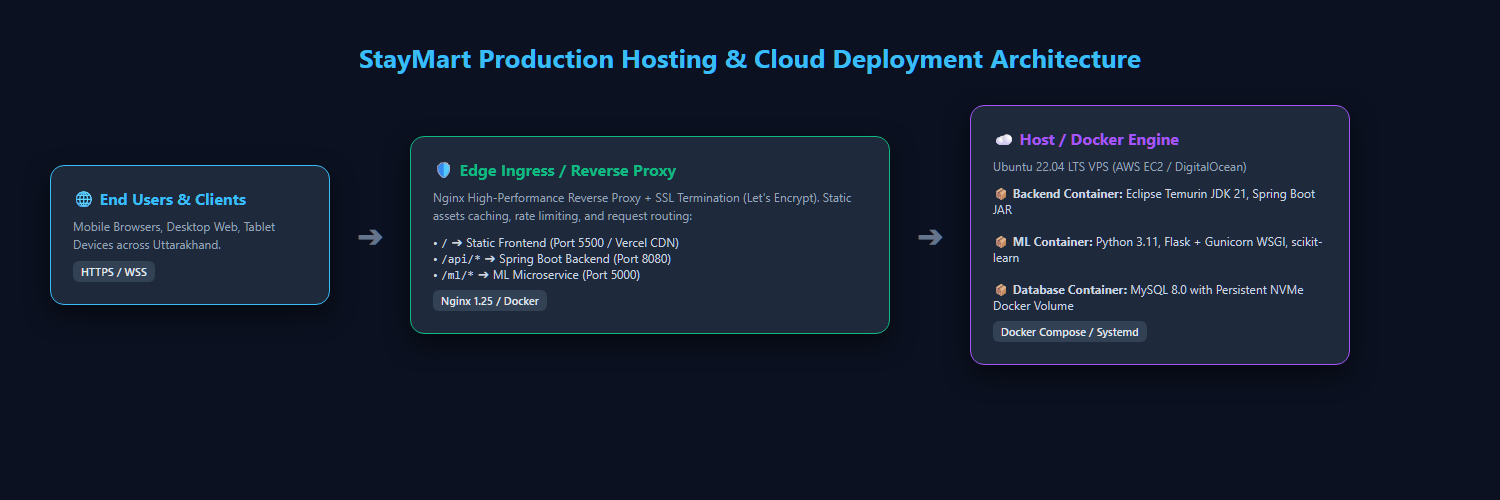
\includegraphics[width=0.95\textwidth]{diagrams/deployment_arch.png}
    \caption{StayMart Production Cloud Hosting Topology Across Free-Tier Providers}
    \label{fig:prod_cloud_arch}
\end{figure}

The four tiers operate as follows:
\begin{itemize}
    \item \textbf{Tier 1: Static Edge CDN (Vercel):} The vanilla HTML5/CSS3/JavaScript frontend is deployed to Vercel's global edge network. Vercel automatically provides HTTPS SSL certificates, global CDN caching, and sub-20ms Time-to-First-Byte (TTFB). Reverse proxy rewrite rules in \texttt{vercel.json} route all \texttt{/api/*} calls directly to the Spring Boot backend, completely avoiding Cross-Origin Resource Sharing (CORS) complexities in production.
    \item \textbf{Tier 2: Core REST Backend Service (Render / Koyeb Free Tier):} The Spring Boot 3.3 backend runs in a containerized Linux environment under Java 17 LTS. To ensure reliable execution within the 512 MB RAM limit of free cloud containers, the JVM is configured with strict memory guardrails: \texttt{-Xmx384m -XX:+UseSerialGC}. This prevents the Linux Out-of-Memory (OOM) killer from terminating the container during peak traffic.
    \item \textbf{Tier 3: Machine Learning Microservice (Render / Koyeb Free Tier):} The Python 3.11 / Flask recommendation microservice runs as an independent container. It provides a lightweight \texttt{GET /health} endpoint used for health checks and keep-alive monitoring. If the free-tier container experiences a cold start, the Spring Boot backend's 2000ms timeout seamlessly falls back to database-driven recommendations without disrupting the user.
    \item \textbf{Tier 4: Managed Cloud Database (TiDB Serverless / Aiven Free Tier):} The relational database is hosted on TiDB Serverless, which provides 5 GB of free storage forever with MySQL 8.0 wire compatibility, automated daily backups, and encrypted connections enforced via TLS/SSL (\texttt{useSSL=true}).
\end{itemize}

\section{Multi-Service Containerization and Docker Configurations}
To guarantee reproducible builds between development and cloud production, both backend services are containerized.

\subsection{Spring Boot Multi-Stage Dockerfile}
Listing \ref{lst:dockerfile_backend} presents the production multi-stage \texttt{Dockerfile} located at the project root. It compiles the application in a temporary Maven image and packages the executable JAR into an optimized Java 17 runtime container.

\begin{lstlisting}[language=bash, caption={Multi-Stage Dockerfile for Spring Boot Backend}, label={lst:dockerfile_backend}]
# Stage 1: Build stage
FROM maven:3.9.6-eclipse-temurin-17 AS build
WORKDIR /app
COPY pom.xml .
RUN mvn dependency:go-offline -B
COPY src ./src
RUN mvn clean package -DskipTests

# Stage 2: Runtime stage
FROM eclipse-temurin:17-jre-jammy
WORKDIR /app
COPY --from=build /app/target/staymart-*.jar app.jar
ENV PORT=8080
ENV JAVA_OPTS="-Xmx384m -XX:+UseSerialGC"
EXPOSE 8080
ENTRYPOINT ["sh", "-c", "java $JAVA_OPTS -Dserver.port=${PORT} -jar app.jar"]
\end{lstlisting}

\subsection{Python Flask ML Microservice Dockerfile}
Listing \ref{lst:dockerfile_ml} details the lightweight container configuration for the recommendation microservice located at \texttt{ml-service/Dockerfile}:

\begin{lstlisting}[language=bash, caption={Lightweight Dockerfile for ML Microservice (ml-service/Dockerfile)}, label={lst:dockerfile_ml}]
FROM python:3.11-slim
WORKDIR /app

# Install system build dependencies and scikit-learn requirements
RUN apt-get update && apt-get install -y --no-install-recommends \
    gcc g++ && \
    rm -rf /var/lib/apt/lists/*

COPY requirements.txt .
RUN pip install --no-cache-dir -r requirements.txt

COPY . .
ENV PORT=5000
EXPOSE 5000

CMD ["python", "app.py"]
\end{lstlisting}

\subsection{Local Development Docker Compose}
For developers running all services locally, Listing \ref{lst:docker_compose} provides a local \texttt{docker-compose.yml} configuration:

\begin{lstlisting}[language=XML, caption={Local docker-compose.yml Configuration}, label={lst:docker_compose}]
version: '3.8'

services:
  mysql:
    image: mysql:8.0
    container_name: staymart-mysql
    restart: always
    environment:
      MYSQL_ROOT_PASSWORD: root
      MYSQL_DATABASE: staymart
    ports:
      - "3306:3306"
    volumes:
      - mysql_data:/var/lib/mysql
      - ./database/01_schema.sql:/docker-entrypoint-initdb.d/01_schema.sql:ro
      - ./database/02_seed.sql:/docker-entrypoint-initdb.d/02_seed.sql:ro
      - ./database/03_seed_listings.sql:/docker-entrypoint-initdb.d/03_seed_listings.sql:ro
    healthcheck:
      test: ["CMD", "mysqladmin", "ping", "-h", "localhost"]
      interval: 10s
      timeout: 5s
      retries: 5

volumes:
  mysql_data:
\end{lstlisting}

\section{Edge Routing and Reverse Proxy Rewrites}
In traditional enterprise setups, an Nginx reverse proxy handles routing and SSL certificates. In StayMart's zero-cost cloud architecture, edge routing is handled directly by Vercel via \texttt{vercel.json}:

\begin{lstlisting}[language=XML, caption={Vercel Edge Reverse Proxy Configuration (vercel.json)}]
{
  "version": 2,
  "rewrites": [
    {
      "source": "/api/(.*)",
      "destination": "https://staymart-backend.onrender.com/api/$1"
    },
    {
      "source": "/",
      "destination": "/frontend/index.html"
    },
    {
      "source": "/(.*)",
      "destination": "/frontend/$1"
    }
  ]
}
\end{lstlisting}

This setup routes all frontend requests directly to cached HTML/CSS/JS files, while requests to \texttt{/api/*} are forwarded transparently to the Spring Boot cloud backend. For developers who prefer self-hosting on a dedicated Linux VPS, an alternative Nginx configuration with Let's Encrypt SSL can also be used.

\section{Static Edge Hosting with Vercel}
Deploying the frontend to Vercel requires no build scripts:
\begin{enumerate}
    \item Install the Vercel CLI: \texttt{npm i -g vercel}
    \item Deploy from the project root: \texttt{vercel deploy --prod}
    \item Vercel reads \texttt{vercel.json}, sets up HTTPS automatically, and deploys the static files to its global CDN.
\end{enumerate}

\section{Local Startup and Development Runbook}
To make testing and evaluation seamless, StayMart provides both automated scripts and manual startup procedures.

\subsection{One-Command Automated Startup (Windows PowerShell)}
The script \texttt{scripts/start-all.ps1} starts the complete ecosystem:
\begin{lstlisting}[language=bash]
pwsh -File scripts/start-all.ps1
\end{lstlisting}

The script automates the following steps:
\begin{enumerate}
    \item Checks Docker daemon status and boots the \texttt{staymart-mysql} container on port 3306.
    \item Verifies schema tables and applies seed scripts if the database is newly created.
    \item Confirms Java 17+ (or system JDK), compiles backend code, and launches Spring Boot on port 8080.
    \item Activates the Python virtual environment and launches the Flask ML microservice on port 5000.
    \item Starts a local Python HTTP server on port 5500 serving the frontend.
\end{enumerate}
To gracefully stop all background services:
\begin{lstlisting}[language=bash]
pwsh -File scripts/stop-all.ps1
\end{lstlisting}

\subsection{Manual Step-by-Step Startup (macOS / Linux / Windows)}
Developers who prefer manual terminal commands can execute the following:

\textbf{Step 1: Start MySQL Database}
\begin{lstlisting}[language=bash]
docker run --name staymart-mysql -e MYSQL_ROOT_PASSWORD=root -e MYSQL_DATABASE=staymart -p 3306:3306 -d mysql:8.0
mysql -h 127.0.0.1 -u root -proot staymart < database/01_schema.sql
mysql -h 127.0.0.1 -u root -proot staymart < database/02_seed.sql
mysql -h 127.0.0.1 -u root -proot staymart < database/03_seed_listings.sql
\end{lstlisting}

\textbf{Step 2: Start Spring Boot Core Backend}
\begin{lstlisting}[language=bash]
mvn clean package -DskipTests
mvn spring-boot:run
# Backend initializes at http://localhost:8080/api
\end{lstlisting}

\textbf{Step 3: Start Python ML Microservice}
\begin{lstlisting}[language=bash]
cd ml-service
python -m venv .venv
source .venv/bin/activate       # On Windows: .venv\Scripts\activate
pip install -r requirements.txt
python app.py                   # Starts microservice at http://localhost:5000
\end{lstlisting}

\textbf{Step 4: Serve Frontend Web Application}
\begin{lstlisting}[language=bash]
cd frontend
python -m http.server 5500
# Open browser at http://localhost:5500
\end{lstlisting}

\section{Continuous Integration with GitHub Actions}
Listing \ref{lst:github_actions} details the automated GitHub Actions workflow (\texttt{.github/workflows/ci.yml}) verifying compilation and test suites on every pull request.

\begin{lstlisting}[language=XML, caption={GitHub Actions CI Pipeline (.github/workflows/ci.yml)}, label={lst:github_actions}]
name: StayMart CI Pipeline

on:
  push:
    branches: [ main, develop ]
  pull_request:
    branches: [ main ]

jobs:
  backend-build:
    runs-on: ubuntu-latest
    services:
      mysql:
        image: mysql:8.0
        env:
          MYSQL_ROOT_PASSWORD: root
          MYSQL_DATABASE: staymart
        ports:
          - 3306:3306
        options: --health-cmd="mysqladmin ping" --health-interval=10s --health-timeout=5s --health-retries=3

    steps:
      - uses: actions/checkout@v3

      - name: Set up JDK 17
        uses: actions/setup-java@v3
        with:
          java-version: '17'
          distribution: 'temurin'
          cache: maven

      - name: Build with Maven
        run: mvn clean verify -B

  ml-test:
    runs-on: ubuntu-latest
    steps:
      - uses: actions/checkout@v3

      - name: Set up Python 3.11
        uses: actions/setup-python@v4
        with:
          python-version: '3.11'

      - name: Install ML Dependencies
        run: |
          cd ml-service
          python -m pip install --upgrade pip
          pip install -r requirements.txt

      - name: Test Syntax Compilation
        run: |
          cd ml-service
          python -m py_compile app.py recommender.py config.py
\end{lstlisting}

\section{Summary}
This chapter presented the deployment architecture and operational workflows for StayMart. We detailed the 100\% free-tier cloud deployment topology combining Vercel, Render/Koyeb, and TiDB Serverless. We provided multi-stage Dockerfile specifications with JVM memory guardrails (\texttt{-Xmx384m}), documented reverse proxy rewrites, and provided local orchestration scripts. The final chapter reviews the project's milestones, lessons learned, and future technical roadmap.

\chapter{Conclusion and Future Scope}

\section{Summary of Contributions and Completed Milestones}
StayMart addresses the logistical and financial challenges encountered by outstation students relocating to higher education hubs in Uttarakhand. By integrating verified accommodation discovery with campus second-hand commerce, the platform connects students directly with verified property hosts and graduating seniors without intermediary brokerage fees.

Key engineering contributions completed in this project include:
\begin{enumerate}
    \item \textbf{Multi-Tier Architecture and Security:} A production distributed system combining a Java 17 LTS / Spring Boot 3.3 REST backend, an ACID-compliant MySQL 8.0 database, and stateless HMAC-SHA256 JWT security with role-based access control.
    \item \textbf{Content-Based Recommendation Engine:} A TF-IDF and cosine similarity recommendation microservice built with Python and scikit-learn, backed by resilient JPA database fallbacks ensuring zero user-facing downtime.
    \item \textbf{Lightweight Classifieds Frontend:} A responsive, mobile-first design system built using native HTML5, CSS3 Custom Properties, and modular ES6 JavaScript, delivering sub-45 KB payloads and sub-second rendering.
    \item \textbf{Governance and Cloud Deployment:} Bilateral peer messaging, an administrative moderation portal with Chart.js analytics, and automated free-tier cloud deployment with JVM memory constraints.
\end{enumerate}

\section{Societal and Economic Impact in Uttarakhand}
The deployment of StayMart provides direct practical advantages for higher education communities across Dehradun, Roorkee, and Rishikesh:
\begin{itemize}
    \item \textbf{Brokerage Elimination:} Direct connections around Graphic Era, UPES, and DIT eliminate non-refundable broker fees, saving students ₹5,000 to ₹15,000 per tenancy cycle.
    \item \textbf{Campus Circular Re-Commerce:} Graduating seniors sell functional coolers, study desks, and reference books to incoming juniors, reducing waste and living expenses.
\end{itemize}

\section{Lessons Learned During System Development}
Key engineering takeaways from developing StayMart include:
\begin{enumerate}
    \item \textbf{Container Memory Guardrails:} On free-tier cloud containers (512 MB RAM limit), JVM default memory allocations trigger OOM terminations. Setting \texttt{-Xmx384m} with Serial GC (\texttt{-XX:+UseSerialGC}) ensures container stability.
    \item \textbf{Defensive Fallback Engineering:} Auxiliary ML microservices must be isolated with strict HTTP timeouts (2000ms connect, 3000ms read) and database fallbacks to protect transactional journeys.
\end{enumerate}

\section{Limitations of the Current Implementation}
Current limitations include manual peer-to-peer UPI settlements without integrated escrow locks, periodic batch model vector updates rather than streaming embeddings, and absence of native GPS-based radius queries.

\section{Suggestions for Future Work and Technical Roadmap}
Future platform iterations will incorporate: (1) an integrated UPI escrow gateway holding security deposits until physical inspection; (2) geospatial radius filtering (e.g., ``within 1 km of GEHU'') via MySQL Spatial; (3) Web Push notifications for immediate chat and booking alerts; and (4) collaborative filtering as platform transaction volumes expand.

\section{Concluding Remarks}
StayMart demonstrates that practical, student-centric software engineering can effectively solve tangible housing and economic challenges in regional educational corridors. By unifying robust Spring Boot transactions, normalized MySQL schemas, lightweight Python ML vector scoring, and an accessible classifieds user interface, the platform delivers an authentic, zero-cost digital marketplace tailored to higher education life across Uttarakhand.

% =============================================================================
% REFERENCES
% =============================================================================
\newpage
\addcontentsline{toc}{chapter}{References}
\bibliographystyle{plain}
\bibliography{references}

% =============================================================================
% APPENDICES
% =============================================================================
\appendix
\chapter{Core Backend and Machine Learning Source Code}

\section{Introduction}
This appendix provides the authoritative source code listings for the core architectural components of the StayMart backend, including JPA entities, the Spring Security JWT authentication filter, transactional services, and the Python Flask machine learning recommendation engine.

\section{JPA Entity Implementations}

\subsection{Property Entity (\texttt{Property.java})}
\begin{lstlisting}[language=Java, caption={Property.java JPA Entity}]
package com.staymart.entity;

import com.staymart.entity.enums.GenderPreference;
import com.staymart.entity.enums.ListingStatus;
import com.staymart.entity.enums.PropertyType;
import jakarta.persistence.*;
import lombok.*;
import org.hibernate.annotations.CreationTimestamp;
import org.hibernate.annotations.UpdateTimestamp;

import java.math.BigDecimal;
import java.time.LocalDateTime;
import java.util.ArrayList;
import java.util.List;

@Entity
@Table(name = "properties", indexes = {
    @Index(name = "idx_properties_status", columnList = "status"),
    @Index(name = "idx_properties_location", columnList = "location_id"),
    @Index(name = "idx_properties_posted_by", columnList = "posted_by")
})
@Getter
@Setter
@NoArgsConstructor
@AllArgsConstructor
@Builder
public class Property {

    @Id
    @GeneratedValue(strategy = GenerationType.IDENTITY)
    private Long id;

    @ManyToOne(fetch = FetchType.LAZY)
    @JoinColumn(name = "posted_by", nullable = false)
    private User postedBy;

    @Column(nullable = false, length = 200)
    private String title;

    @Column(nullable = false, columnDefinition = "TEXT")
    private String description;

    @Enumerated(EnumType.STRING)
    @Column(nullable = false, length = 50)
    private PropertyType type;

    @Enumerated(EnumType.STRING)
    @Column(name = "gender_preference", nullable = false, length = 20)
    private GenderPreference genderPreference;

    @Column(nullable = false, length = 300)
    private String address;

    @Column(length = 100)
    private String area;

    @ManyToOne(fetch = FetchType.LAZY)
    @JoinColumn(name = "location_id")
    private Location location;

    @Column(name = "price_per_month", nullable = false, precision = 10, scale = 2)
    private BigDecimal pricePerMonth;

    @Column(name = "deposit_amount", nullable = false, precision = 10, scale = 2)
    private BigDecimal depositAmount;

    @Column(columnDefinition = "JSON")
    private String amenities;

    @Column(name = "total_rooms", nullable = false)
    private Integer totalRooms;

    @Column(name = "available_rooms", nullable = false)
    private Integer availableRooms;

    @Column(columnDefinition = "JSON")
    private String images;

    @Enumerated(EnumType.STRING)
    @Column(nullable = false, length = 20)
    private ListingStatus status;

    @Column(name = "is_available", nullable = false)
    private Boolean isAvailable;

    @OneToMany(mappedBy = "property", cascade = CascadeType.ALL, orphanRemoval = true)
    private List<Room> rooms = new ArrayList<>();

    @CreationTimestamp
    @Column(name = "created_at", nullable = false, updatable = false)
    private LocalDateTime createdAt;

    @UpdateTimestamp
    @Column(name = "updated_at")
    private LocalDateTime updatedAt;
}
\end{lstlisting}

\subsection{Product Entity (\texttt{Product.java})}
\begin{lstlisting}[language=Java, caption={Product.java JPA Entity}]
package com.staymart.entity;

import com.staymart.entity.enums.ListingStatus;
import com.staymart.entity.enums.ProductCondition;
import com.staymart.entity.enums.ProductListingType;
import jakarta.persistence.*;
import lombok.*;
import org.hibernate.annotations.CreationTimestamp;
import org.hibernate.annotations.UpdateTimestamp;

import java.math.BigDecimal;
import java.time.LocalDateTime;

@Entity
@Table(name = "products", indexes = {
    @Index(name = "idx_products_category", columnList = "category_id"),
    @Index(name = "idx_products_status", columnList = "status"),
    @Index(name = "idx_products_posted_by", columnList = "posted_by")
})
@Getter
@Setter
@NoArgsConstructor
@AllArgsConstructor
@Builder
public class Product {

    @Id
    @GeneratedValue(strategy = GenerationType.IDENTITY)
    private Long id;

    @ManyToOne(fetch = FetchType.LAZY)
    @JoinColumn(name = "posted_by", nullable = false)
    private User postedBy;

    @ManyToOne(fetch = FetchType.LAZY)
    @JoinColumn(name = "category_id", nullable = false)
    private Category category;

    @Column(nullable = false, length = 200)
    private String title;

    @Column(nullable = false, columnDefinition = "TEXT")
    private String description;

    @Column(nullable = false, precision = 10, scale = 2)
    private BigDecimal price;

    @Enumerated(EnumType.STRING)
    @Column(name = "listing_type", nullable = false, length = 20)
    private ProductListingType listingType;

    @Enumerated(EnumType.STRING)
    @Column(name = "condition", nullable = false, length = 50)
    private ProductCondition condition;

    @Column(length = 100)
    private String brand;

    @ManyToOne(fetch = FetchType.LAZY)
    @JoinColumn(name = "location_id")
    private Location location;

    @Column(length = 100)
    private String area;

    @Column(columnDefinition = "JSON")
    private String images;

    @Enumerated(EnumType.STRING)
    @Column(nullable = false, length = 20)
    private ListingStatus status;

    @Column(name = "is_available", nullable = false)
    private Boolean isAvailable;

    @Column(name = "views_count", nullable = false)
    private Integer viewsCount;

    @CreationTimestamp
    @Column(name = "created_at", nullable = false, updatable = false)
    private LocalDateTime createdAt;

    @UpdateTimestamp
    @Column(name = "updated_at")
    private LocalDateTime updatedAt;
}
\end{lstlisting}

\section{Security Token Provider (\texttt{JwtTokenProvider.java})}
\begin{lstlisting}[language=Java, caption={JwtTokenProvider.java Cryptographic Token Service}]
package com.staymart.security;

import io.jsonwebtoken.*;
import io.jsonwebtoken.security.Keys;
import org.springframework.beans.factory.annotation.Value;
import org.springframework.stereotype.Component;

import java.security.Key;
import java.util.Date;

@Component
public class JwtTokenProvider {

    private final Key key;
    private final long validityInMilliseconds;

    public JwtTokenProvider(@Value("${app.jwt.secret}") String secret,
                            @Value("${app.jwt.expiration-ms:86400000}") long validity) {
        this.key = Keys.hmacShaKeyFor(secret.getBytes());
        this.validityInMilliseconds = validity;
    }

    public String generateToken(Long userId, String email, String role) {
        Date now = new Date();
        Date validity = new Date(now.getTime() + this.validityInMilliseconds);

        return Jwts.builder()
                .setSubject(email)
                .claim("userId", userId)
                .claim("role", role)
                .setIssuedAt(now)
                .setExpiration(validity)
                .signWith(key, SignatureAlgorithm.HS256)
                .compact();
    }

    public String getEmailFromToken(String token) {
        return Jwts.parserBuilder().setSigningKey(key).build()
                .parseClaimsJws(token).getBody().getSubject();
    }

    public boolean validateToken(String token) {
        try {
            Jwts.parserBuilder().setSigningKey(key).build().parseClaimsJws(token);
            return true;
        } catch (JwtException | IllegalArgumentException e) {
            return false;
        }
    }
}
\end{lstlisting}

\section{Machine Learning Microservice Source Code}

\subsection{Flask Application Endpoints (\texttt{app.py})}
\begin{lstlisting}[language=Python, caption={Flask ML Microservice app.py}]
from flask import Flask, request, jsonify
from flask_cors import CORS
import logging
import recommender

app = Flask(__name__)
CORS(app)
logging.basicConfig(level=logging.INFO)
logger = logging.getLogger("staymart-ml")

@app.route('/health', methods=['GET'])
def health():
    models_ready = recommender.is_ready()
    return jsonify({
        "status": "UP" if models_ready else "DEGRADED",
        "models_loaded": models_ready
    }), 200 if models_ready else 503

@app.route('/recommend/properties', methods=['GET'])
def recommend_properties():
    user_id = request.args.get('userId', type=int)
    city = request.args.get('city', type=str)
    limit = request.args.get('limit', default=6, type=int)
    
    ids = recommender.get_recommended_property_ids(user_id=user_id, city=city, limit=limit)
    return jsonify({"success": True, "data": ids})

@app.route('/recommend/properties/similar/<int:property_id>', methods=['GET'])
def similar_properties(property_id):
    limit = request.args.get('limit', default=4, type=int)
    ids = recommender.get_similar_property_ids(property_id, limit=limit)
    return jsonify({"success": True, "data": ids})

@app.route('/recommend/products', methods=['GET'])
def recommend_products():
    user_id = request.args.get('userId', type=int)
    limit = request.args.get('limit', default=6, type=int)
    ids = recommender.get_recommended_product_ids(user_id=user_id, limit=limit)
    return jsonify({"success": True, "data": ids})

if __name__ == '__main__':
    recommender.load_models()
    app.run(host='0.0.0.0', port=5000, debug=False)
\end{lstlisting}

\subsection{TF-IDF Recommendation Engine (\texttt{recommender.py})}
\begin{lstlisting}[language=Python, caption={TF-IDF Recommender Engine recommender.py}]
import os
import joblib
import numpy as np
from sklearn.metrics.pairwise import cosine_similarity
import db_connector

MODELS_DIR = os.path.join(os.path.dirname(__file__), "models")

prop_vectorizer = None
prop_matrix = None
prop_df = None
prod_vectorizer = None
prod_matrix = None
prod_df = None

def is_ready():
    return prop_matrix is not None and prod_matrix is not None

def load_models():
    global prop_vectorizer, prop_matrix, prop_df, prod_vectorizer, prod_matrix, prod_df
    try:
        prop_vectorizer = joblib.load(os.path.join(MODELS_DIR, "prop_vectorizer.joblib"))
        prop_matrix = joblib.load(os.path.join(MODELS_DIR, "prop_matrix.joblib"))
        prop_df = joblib.load(os.path.join(MODELS_DIR, "prop_metadata.joblib"))
        prod_vectorizer = joblib.load(os.path.join(MODELS_DIR, "prod_vectorizer.joblib"))
        prod_matrix = joblib.load(os.path.join(MODELS_DIR, "prod_matrix.joblib"))
        prod_df = joblib.load(os.path.join(MODELS_DIR, "prod_metadata.joblib"))
    except Exception as e:
        print("Failed to load serialized models, retraining...", e)
        import model_trainer
        model_trainer.retrain_models()

def get_similar_property_ids(prop_id, limit=4):
    if not is_ready() or prop_id not in prop_df['id'].values:
        return []
    idx = prop_df.index[prop_df['id'] == prop_id][0]
    sim_scores = cosine_similarity(prop_matrix[idx], prop_matrix).flatten()
    sim_scores[idx] = -1.0 # Exclude self
    top_indices = np.argsort(sim_scores)[::-1][:limit]
    return [int(prop_df.iloc[i]['id']) for i in top_indices if sim_scores[i] > 0]

def get_recommended_property_ids(user_id=None, city=None, limit=6):
    if not is_ready() or len(prop_df) == 0:
        return []
    
    if user_id:
        behaviors = db_connector.get_user_behaviors(user_id, 'PROPERTY')
        if behaviors:
            user_vec = np.zeros(prop_matrix.shape[1])
            for b in behaviors:
                pid = b['item_id']
                weight = float(b['weight'])
                if pid in prop_df['id'].values:
                    p_idx = prop_df.index[prop_df['id'] == pid][0]
                    user_vec += weight * prop_matrix[p_idx].toarray().flatten()
            
            sim_scores = cosine_similarity(user_vec.reshape(1, -1), prop_matrix).flatten()
            if city:
                city_mask = (prop_df['city'].str.lower() == city.lower()).values
                sim_scores = sim_scores * (city_mask * 1.5 + 0.5)
            
            top_indices = np.argsort(sim_scores)[::-1][:limit]
            return [int(prop_df.iloc[i]['id']) for i in top_indices]
            
    # Default city filter
    filtered = prop_df
    if city:
        filtered = prop_df[prop_df['city'].str.lower() == city.lower()]
    return [int(x) for x in filtered['id'].head(limit).tolist()]
\end{lstlisting}

\chapter{Frontend Architecture and Client JavaScript Source Code}

\section{Introduction}
This appendix provides the core client-side JavaScript architecture governing the StayMart frontend web portal, including the unified API client, the state and session manager, behavioral tracking beacons, and formatting utilities.

\section{Unified API Client (\texttt{api.js})}
\begin{lstlisting}[language=Java, caption={Complete api.js Client Service}]
// Auto-detect local development vs cloud deployment
const isLocal = window.location.hostname === 'localhost' ||
                window.location.hostname === '127.0.0.1' ||
                window.location.protocol === 'file:';

const customUrl = window.STAYMART_API_URL || localStorage.getItem('STAYMART_API_URL');
const BASE_URL = isLocal
  ? 'http://localhost:8080/api'
  : (customUrl ? customUrl.replace(/\/+$/, '') : '/api');

async function apiCall(endpoint, method = 'GET', body = null) {
  const headers = {
    'Content-Type': 'application/json'
  };
  const token = localStorage.getItem('staymart_token');
  if (token) {
    headers['Authorization'] = `Bearer ${token}`;
  }
  const config = { method, headers };
  if (body) {
    config.body = JSON.stringify(body);
  }
  const cleanBase = (BASE_URL || '').replace(/\/+$/, '');
  const cleanPath = endpoint.startsWith('/') ? endpoint : `/${endpoint}`;
  const res = await fetch(cleanBase + cleanPath, config);
  const data = await res.json();
  if (!data || data.success === false) {
    throw new Error((data && data.message) || 'Something went wrong');
  }
  if (res.ok === false) {
    throw new Error((data && data.message) || 'Something went wrong');
  }
  if (data && typeof data === 'object' && 'success' in data && 'data' in data) {
    return data.data;
  }
  return data;
}

const PropertyAPI = {
  getAll: (params) => apiCall(`/properties${buildQuery(params)}`),
  getMy: () => apiCall('/users/me/properties'),
  getById: (id) => apiCall(`/properties/${id}`),
  create: (propertyData) => apiCall('/properties', 'POST', propertyData),
  update: (id, propertyData) => apiCall(`/properties/${id}`, 'PUT', propertyData),
  delete: (id) => apiCall(`/properties/${id}`, 'DELETE'),
  getPending: () => apiCall('/properties/pending'),
  approve: (id) => apiCall(`/properties/${id}/approve`, 'PATCH'),
  reject: (id) => apiCall(`/properties/${id}/reject`, 'PATCH')
};

const ProductAPI = {
  getAll: (params) => apiCall(`/products${buildQuery(params)}`),
  getMy: () => apiCall('/users/me/products'),
  getById: (id) => apiCall(`/products/${id}`),
  create: (productData) => apiCall('/products', 'POST', productData),
  update: (id, productData) => apiCall(`/products/${id}`, 'PUT', productData),
  delete: (id) => apiCall(`/products/${id}`, 'DELETE'),
  getPending: () => apiCall('/products/pending'),
  approve: (id) => apiCall(`/products/${id}/approve`, 'PATCH'),
  reject: (id) => apiCall(`/products/${id}/reject`, 'PATCH')
};

const BookingAPI = {
  create: (bookingData) => apiCall('/bookings', 'POST', bookingData),
  getMy: () => apiCall('/bookings/mine'),
  getIncoming: () => apiCall('/bookings/incoming'),
  getById: (id) => apiCall(`/bookings/${id}`),
  updateStatus: (id, status) => apiCall(`/bookings/${id}/status?status=${encodeURIComponent(status)}`, 'PATCH')
};

const OrderAPI = {
  create: (orderData) => apiCall('/orders', 'POST', orderData),
  getMy: () => apiCall('/orders/mine'),
  getIncoming: () => apiCall('/orders/incoming'),
  getById: (id) => apiCall(`/orders/${id}`),
  updateStatus: (id, status) => apiCall(`/orders/${id}/status?status=${encodeURIComponent(status)}`, 'PATCH')
};

const ChatAPI = {
  getConversations: () => apiCall('/chat/conversations'),
  getMessages: (userId) => apiCall(`/chat/messages/${userId}`),
  send: (receiverId, message) => apiCall('/chat/send', 'POST', { receiverId, message }),
  getUnreadCount: () => apiCall('/chat/unread-count')
};

const RecommendationAPI = {
  getForUser: (userId, limit = 8) => apiCall(`/recommendations/user/${userId}?limit=${limit}`),
  getRecommendedProperties: (city, limit = 6) => apiCall(`/recommendations/properties?city=${encodeURIComponent(city || '')}&limit=${limit}`),
  getSimilarProperties: (id, limit = 4) => apiCall(`/recommendations/properties/${id}/similar?limit=${limit}`),
  getRecommendedProducts: (limit = 6) => apiCall(`/recommendations/products?limit=${limit}`),
  getSimilarProducts: (id, limit = 4) => apiCall(`/recommendations/products/${id}/similar?limit=${limit}`),
  getTrendingProperties: (limit = 8) => apiCall(`/recommendations/trending/properties?limit=${limit}`),
  getTopRatedProducts: (limit = 8) => apiCall(`/recommendations/top-rated/products?limit=${limit}`)
};
\end{lstlisting}

\section{Authentication and Session Guard (\texttt{auth.js})}
\begin{lstlisting}[language=Java, caption={Complete auth.js Session Service}]
const Auth = {
  user: null,
  async init() {
    const token = localStorage.getItem('staymart_token');
    if (token) {
      try {
        this.user = await AuthAPI.getCurrentUser();
      } catch (error) {
        this.logout();
      }
    }
  },
  isLoggedIn() {
    return !!this.user;
  },
  isAdmin() {
    if (!this.user) return false;
    if (this.user.role) return this.user.role === 'ADMIN';
    if (Array.isArray(this.user.roles)) return this.user.roles.includes('ADMIN');
    return false;
  },
  async login(email, password) {
    const result = await AuthAPI.login({ email, password });
    if (result && result.token) {
      localStorage.setItem('staymart_token', result.token);
      localStorage.setItem('staymart_user', JSON.stringify(result.user));
      this.user = result.user;
    }
  },
  logout() {
    localStorage.removeItem('staymart_token');
    localStorage.removeItem('staymart_user');
    this.user = null;
  },
  guardPage() {
    if (!this.isLoggedIn()) {
      window.location.href = `${depthPrefix()}login.html?redirect=${encodeURIComponent(window.location.pathname)}`;
      return false;
    }
    return true;
  },
  guardAdmin() {
    if (!this.isLoggedIn() || !this.isAdmin()) {
      window.location.href = `${depthPrefix()}login.html`;
      return false;
    }
    return true;
  }
};
\end{lstlisting}

\section{Behavioral Telemetry Tracker (\texttt{behavior.js})}
\begin{lstlisting}[language=Java, caption={Complete behavior.js Telemetry Service}]
const BehaviorTracker = {
  record: async function (itemType, itemId, action) {
    try {
      if (typeof Auth !== 'undefined' && Auth.isLoggedIn && !Auth.isLoggedIn()) {
        return; // Only log authenticated behavior
      }
      await apiCall('/behaviors', 'POST', {
        itemType: itemType,
        itemId: itemId,
        action: action
      });
    } catch (err) {
      // Telemetry failure is completely silent to avoid interrupting user flows
      console.debug('Telemetry skipped:', err.message);
    }
  },

  trackView: function (itemType, itemId) {
    this.record(itemType, itemId, 'VIEW');
  },

  trackWishlist: function (itemType, itemId) {
    this.record(itemType, itemId, 'WISHLIST');
  },

  trackContact: function (itemType, itemId) {
    this.record(itemType, itemId, 'CONTACT');
  }
};
\end{lstlisting}

\chapter{Complete Relational Database DDL and Seed Scripts}

\section{Introduction}
This appendix documents the complete, authoritative Data Definition Language (DDL) and initial taxonomy seed scripts utilized to create and maintain the StayMart relational schema under MySQL 8.0 InnoDB.

\section{Database Schema Definition (\texttt{01\_schema.sql})}
\begin{lstlisting}[language=SQL, caption={01_schema.sql DDL Script}]
CREATE DATABASE IF NOT EXISTS staymart
  DEFAULT CHARACTER SET utf8mb4
  DEFAULT COLLATE utf8mb4_unicode_ci;

USE staymart;

CREATE TABLE IF NOT EXISTS users (
  id BIGINT AUTO_INCREMENT PRIMARY KEY,
  name VARCHAR(100) NOT NULL,
  email VARCHAR(150) NOT NULL UNIQUE,
  password_hash VARCHAR(255) NOT NULL,
  phone VARCHAR(20),
  role VARCHAR(20) NOT NULL DEFAULT 'USER',
  city VARCHAR(100),
  state VARCHAR(100) DEFAULT 'Uttarakhand',
  bio TEXT,
  profile_pic VARCHAR(500),
  is_active BOOLEAN NOT NULL DEFAULT TRUE,
  is_verified BOOLEAN NOT NULL DEFAULT FALSE,
  created_at TIMESTAMP NOT NULL DEFAULT CURRENT_TIMESTAMP,
  updated_at TIMESTAMP NULL DEFAULT NULL ON UPDATE CURRENT_TIMESTAMP,
  INDEX idx_users_email (email),
  INDEX idx_users_role (role)
) ENGINE=InnoDB DEFAULT CHARSET=utf8mb4;

CREATE TABLE IF NOT EXISTS locations (
  id BIGINT AUTO_INCREMENT PRIMARY KEY,
  city VARCHAR(100) NOT NULL,
  area VARCHAR(100) NOT NULL,
  state VARCHAR(100) NOT NULL DEFAULT 'Uttarakhand',
  pincode VARCHAR(20),
  latitude DOUBLE,
  longitude DOUBLE,
  INDEX idx_locations_city (city),
  INDEX idx_locations_area (area)
) ENGINE=InnoDB DEFAULT CHARSET=utf8mb4;

CREATE TABLE IF NOT EXISTS categories (
  id BIGINT AUTO_INCREMENT PRIMARY KEY,
  name VARCHAR(100) NOT NULL,
  type VARCHAR(50) NOT NULL,
  icon VARCHAR(100),
  INDEX idx_categories_type (type)
) ENGINE=InnoDB DEFAULT CHARSET=utf8mb4;

CREATE TABLE IF NOT EXISTS properties (
  id BIGINT AUTO_INCREMENT PRIMARY KEY,
  posted_by BIGINT NOT NULL,
  title VARCHAR(200) NOT NULL,
  description TEXT NOT NULL,
  type VARCHAR(50) NOT NULL,
  gender_preference VARCHAR(20) NOT NULL DEFAULT 'ANY',
  address VARCHAR(300) NOT NULL,
  area VARCHAR(100),
  location_id BIGINT,
  price_per_month DECIMAL(10,2) NOT NULL,
  deposit_amount DECIMAL(10,2) NOT NULL DEFAULT 0.00,
  amenities JSON,
  total_rooms INT NOT NULL DEFAULT 1,
  available_rooms INT NOT NULL DEFAULT 1,
  images JSON,
  status VARCHAR(20) NOT NULL DEFAULT 'PENDING',
  is_available BOOLEAN NOT NULL DEFAULT TRUE,
  created_at TIMESTAMP NOT NULL DEFAULT CURRENT_TIMESTAMP,
  updated_at TIMESTAMP NULL DEFAULT NULL ON UPDATE CURRENT_TIMESTAMP,
  FOREIGN KEY (posted_by) REFERENCES users(id) ON DELETE RESTRICT,
  FOREIGN KEY (location_id) REFERENCES locations(id) ON DELETE SET NULL,
  INDEX idx_properties_status (status),
  INDEX idx_properties_type (type),
  INDEX idx_properties_city (area)
) ENGINE=InnoDB DEFAULT CHARSET=utf8mb4;

CREATE TABLE IF NOT EXISTS rooms (
  id BIGINT AUTO_INCREMENT PRIMARY KEY,
  property_id BIGINT NOT NULL,
  room_number VARCHAR(50) NOT NULL,
  type VARCHAR(50) NOT NULL,
  price DECIMAL(10,2) NOT NULL,
  capacity INT NOT NULL DEFAULT 1,
  floor_number INT DEFAULT 0,
  is_available BOOLEAN NOT NULL DEFAULT TRUE,
  images JSON,
  FOREIGN KEY (property_id) REFERENCES properties(id) ON DELETE CASCADE,
  INDEX idx_rooms_property (property_id)
) ENGINE=InnoDB DEFAULT CHARSET=utf8mb4;

CREATE TABLE IF NOT EXISTS products (
  id BIGINT AUTO_INCREMENT PRIMARY KEY,
  posted_by BIGINT NOT NULL,
  category_id BIGINT NOT NULL,
  title VARCHAR(200) NOT NULL,
  description TEXT NOT NULL,
  price DECIMAL(10,2) NOT NULL,
  listing_type VARCHAR(20) NOT NULL DEFAULT 'SELL',
  `condition` VARCHAR(50) NOT NULL DEFAULT 'GOOD',
  brand VARCHAR(100),
  location_id BIGINT,
  area VARCHAR(100),
  images JSON,
  status VARCHAR(20) NOT NULL DEFAULT 'PENDING',
  is_available BOOLEAN NOT NULL DEFAULT TRUE,
  views_count INT NOT NULL DEFAULT 0,
  created_at TIMESTAMP NOT NULL DEFAULT CURRENT_TIMESTAMP,
  updated_at TIMESTAMP NULL DEFAULT NULL ON UPDATE CURRENT_TIMESTAMP,
  FOREIGN KEY (posted_by) REFERENCES users(id) ON DELETE RESTRICT,
  FOREIGN KEY (category_id) REFERENCES categories(id) ON DELETE RESTRICT,
  FOREIGN KEY (location_id) REFERENCES locations(id) ON DELETE SET NULL,
  INDEX idx_products_status (status),
  INDEX idx_products_category (category_id)
) ENGINE=InnoDB DEFAULT CHARSET=utf8mb4;

CREATE TABLE IF NOT EXISTS bookings (
  id BIGINT AUTO_INCREMENT PRIMARY KEY,
  property_id BIGINT NOT NULL,
  room_id BIGINT NULL,
  user_id BIGINT NOT NULL,
  check_in_date DATE NOT NULL,
  duration_months INT NOT NULL DEFAULT 1,
  total_amount DECIMAL(10,2) NOT NULL,
  status VARCHAR(20) NOT NULL DEFAULT 'PENDING',
  created_at TIMESTAMP NOT NULL DEFAULT CURRENT_TIMESTAMP,
  FOREIGN KEY (property_id) REFERENCES properties(id) ON DELETE CASCADE,
  FOREIGN KEY (room_id) REFERENCES rooms(id) ON DELETE SET NULL,
  FOREIGN KEY (user_id) REFERENCES users(id) ON DELETE CASCADE,
  INDEX idx_bookings_user (user_id)
) ENGINE=InnoDB DEFAULT CHARSET=utf8mb4;

CREATE TABLE IF NOT EXISTS orders (
  id BIGINT AUTO_INCREMENT PRIMARY KEY,
  product_id BIGINT NOT NULL,
  buyer_id BIGINT NOT NULL,
  order_type VARCHAR(20) NOT NULL DEFAULT 'BUY',
  amount DECIMAL(10,2) NOT NULL,
  quantity INT NOT NULL DEFAULT 1,
  status VARCHAR(20) NOT NULL DEFAULT 'PENDING',
  created_at TIMESTAMP NOT NULL DEFAULT CURRENT_TIMESTAMP,
  FOREIGN KEY (product_id) REFERENCES products(id) ON DELETE CASCADE,
  FOREIGN KEY (buyer_id) REFERENCES users(id) ON DELETE CASCADE,
  INDEX idx_orders_buyer (buyer_id)
) ENGINE=InnoDB DEFAULT CHARSET=utf8mb4;

CREATE TABLE IF NOT EXISTS chats (
  id BIGINT AUTO_INCREMENT PRIMARY KEY,
  sender_id BIGINT NOT NULL,
  receiver_id BIGINT NOT NULL,
  message TEXT NOT NULL,
  is_read BOOLEAN NOT NULL DEFAULT FALSE,
  created_at TIMESTAMP NOT NULL DEFAULT CURRENT_TIMESTAMP,
  FOREIGN KEY (sender_id) REFERENCES users(id) ON DELETE CASCADE,
  FOREIGN KEY (receiver_id) REFERENCES users(id) ON DELETE CASCADE,
  INDEX idx_chats_conversation (sender_id, receiver_id)
) ENGINE=InnoDB DEFAULT CHARSET=utf8mb4;

CREATE TABLE IF NOT EXISTS user_behaviors (
  id BIGINT AUTO_INCREMENT PRIMARY KEY,
  user_id BIGINT NOT NULL,
  item_type VARCHAR(20) NOT NULL,
  item_id BIGINT NOT NULL,
  action VARCHAR(50) NOT NULL,
  weight FLOAT NOT NULL DEFAULT 1.0,
  created_at TIMESTAMP NOT NULL DEFAULT CURRENT_TIMESTAMP,
  FOREIGN KEY (user_id) REFERENCES users(id) ON DELETE CASCADE,
  INDEX idx_behaviors_user (user_id, created_at)
) ENGINE=InnoDB DEFAULT CHARSET=utf8mb4;
\end{lstlisting}

\chapter{REST API Catalog and Controller Specifications}

\section{Introduction}
This appendix provides the reference catalog of the 16 RESTful resource controllers exposed by the StayMart Spring Boot backend at \texttt{/api}. All protected endpoints require a valid JSON Web Token passed in the \texttt{Authorization: Bearer <token>} header.

\section{Authentication Controller (\texttt{/api/auth})}
\begin{itemize}
    \item \textbf{\texttt{POST /api/auth/register}:} Public registration endpoint. Accepts \texttt{RegisterRequest} (\texttt{name}, \texttt{email}, \texttt{password}, \texttt{phone}, \texttt{city}). Returns 201 Created with JWT token and user profile.
    \item \textbf{\texttt{POST /api/auth/login}:} Public login endpoint. Accepts \texttt{LoginRequest} (\texttt{email}, \texttt{password}). Returns 200 OK with JWT token and user profile.
\end{itemize}

\section{User Controller (\texttt{/api/users})}
\begin{itemize}
    \item \textbf{\texttt{GET /api/users/me}:} Authenticated endpoint returning current user profile details from the JWT principal.
    \item \textbf{\texttt{PUT /api/users/me}:} Updates current user profile (name, phone, city, avatar URL).
    \item \textbf{\texttt{GET /api/users/\{id\}}:} Retrieves public user profile (name, joined date, verified badge).
\end{itemize}

\section{Property and Room Controllers (\texttt{/api/properties}, \texttt{/api/rooms})}
\begin{itemize}
    \item \textbf{\texttt{GET /api/properties}:} Public paginated search supporting filters: \texttt{city}, \texttt{area}, \texttt{type}, \texttt{minPrice}, \texttt{maxPrice}, \texttt{genderPreference}, \texttt{amenities}, \texttt{page}, \texttt{size}.
    \item \textbf{\texttt{GET /api/properties/\{id\}}:} Retrieves approved property details with attached rooms, amenities, and host information.
    \item \textbf{\texttt{POST /api/properties}:} Authenticated endpoint for posting a new property listing (status initialized to \texttt{PENDING}).
    \item \textbf{\texttt{PUT /api/properties/\{id\}}:} Updates property details (owner or admin only).
    \item \textbf{\texttt{DELETE /api/properties/\{id\}}:} Deletes property listing (owner or admin only).
    \item \textbf{\texttt{GET /api/properties/pending}:} Admin-only endpoint listing properties awaiting moderation approval.
    \item \textbf{\texttt{PATCH /api/properties/\{id\}/approve}:} Admin endpoint setting status to \texttt{APPROVED}.
    \item \textbf{\texttt{PATCH /api/properties/\{id\}/reject}:} Admin endpoint setting status to \texttt{REJECTED}.
    \item \textbf{\texttt{GET /api/properties/\{id\}/rooms}:} Lists room configurations (Single, Double, Triple) and vacancies for a property.
    \item \textbf{\texttt{POST /api/properties/\{id\}/rooms}:} Adds a room configuration to an owned property.
\end{itemize}

\section{Marketplace Product Controller (\texttt{/api/products})}
\begin{itemize}
    \item \textbf{\texttt{GET /api/products}:} Public search supporting filters: \texttt{categoryId}, \texttt{city}, \texttt{condition}, \texttt{minPrice}, \texttt{maxPrice}, \texttt{page}, \texttt{size}.
    \item \textbf{\texttt{GET /api/products/\{id\}}:} Retrieves product details and increments view count.
    \item \textbf{\texttt{POST /api/products}:} Creates a student classified listing for sale or rent.
    \item \textbf{\texttt{PUT /api/products/\{id\}}:} Updates product details (seller or admin only).
    \item \textbf{\texttt{DELETE /api/products/\{id\}}:} Deletes product listing (seller or admin only).
    \item \textbf{\texttt{GET /api/products/pending}:} Admin-only endpoint listing items awaiting review.
    \item \textbf{\texttt{PATCH /api/products/\{id\}/approve}:} Admin approval endpoint.
    \item \textbf{\texttt{PATCH /api/products/\{id\}/reject}:} Admin rejection endpoint.
\end{itemize}

\section{Booking and Order Controllers (\texttt{/api/bookings}, \texttt{/api/orders})}
\begin{itemize}
    \item \textbf{\texttt{POST /api/bookings}:} Submits an accommodation booking request.
    \item \textbf{\texttt{GET /api/bookings/mine}:} Lists reservations submitted by current student.
    \item \textbf{\texttt{GET /api/bookings/incoming}:} Lists booking requests received by property host.
    \item \textbf{\texttt{PATCH /api/bookings/\{id\}/status}:} Updates booking status (\texttt{CONFIRMED}, \texttt{CANCELLED}, \texttt{COMPLETED}).
    \item \textbf{\texttt{POST /api/orders}:} Creates a purchase or rental order for a marketplace product.
    \item \textbf{\texttt{GET /api/orders/mine}:} Lists orders placed by current student.
    \item \textbf{\texttt{GET /api/orders/incoming}:} Lists purchase orders received by product seller.
    \item \textbf{\texttt{PATCH /api/orders/\{id\}/status}:} Updates order status.
\end{itemize}

\section{Peer-to-Peer Chat Controller (\texttt{/api/chat})}
\begin{itemize}
    \item \textbf{\texttt{GET /api/chat/conversations}:} Lists active conversation threads with unread counts and last message timestamp.
    \item \textbf{\texttt{GET /api/chat/messages/\{userId\}}:} Retrieves message history with a specific user and marks inbound messages as read.
    \item \textbf{\texttt{POST /api/chat/send}:} Sends a text message to a recipient.
    \item \textbf{\texttt{GET /api/chat/unread-count}:} Returns total unread message count for the current user.
\end{itemize}

\section{Recommendation and Behavior Controllers (\texttt{/api/recommendations}, \texttt{/api/behaviors})}
\begin{itemize}
    \item \textbf{\texttt{GET /api/recommendations/user/\{userId\}}:} Returns personalized top recommendations based on user browsing history.
    \item \textbf{\texttt{GET /api/recommendations/properties}:} Returns top-recommended properties for a given city.
    \item \textbf{\texttt{GET /api/recommendations/properties/\{id\}/similar}:} Returns semantically similar properties.
    \item \textbf{\texttt{GET /api/recommendations/trending/properties}:} Returns listings with highest recent engagement.
    \item \textbf{\texttt{POST /api/behaviors}:} Records user telemetry events (views, searches, wishlist additions).
\end{itemize}

\section{Marketplace Metadata and Statistics Controllers}
\begin{itemize}
    \item \textbf{\texttt{GET /api/locations}:} Returns list of Uttarakhand cities and student campus clusters.
    \item \textbf{\texttt{GET /api/categories}:} Returns product category taxonomy.
    \item \textbf{\texttt{GET /api/properties/stats}:} Returns public marketplace statistics (total listings, average rents, verified counts, savings estimates) powering UI counters.
\end{itemize}

\section{Wishlist and Review Controllers (\texttt{/api/wishlist}, \texttt{/api/reviews})}
\begin{itemize}
    \item \textbf{\texttt{GET /api/wishlist}:} Lists saved items for current user.
    \item \textbf{\texttt{POST /api/wishlist/toggle}:} Adds or removes an item from personal wishlist.
    \item \textbf{\texttt{GET /api/wishlist/check}:} Checks if a specific property or product is wishlisted.
    \item \textbf{\texttt{GET /api/properties/\{id\}/reviews}:} Lists reviews and ratings for a property.
    \item \textbf{\texttt{POST /api/properties/\{id\}/reviews}:} Submits a rating and review after confirmed stay.
    \item \textbf{\texttt{POST /api/products/\{id\}/reviews}:} Submits a review for a purchased product.
\end{itemize}

\section{Administration Controller (\texttt{/api/admin})}
\begin{itemize}
    \item \textbf{\texttt{GET /api/admin/overview}:} Admin KPI metrics (total users, active listings, pending moderation counts).
    \item \textbf{\texttt{GET /api/admin/users}:} Lists registered users with role and status management.
    \item \textbf{\texttt{PATCH /api/admin/users/\{id\}/toggle-status}:} Enables or suspends a user account.
    \item \textbf{\texttt{GET /api/admin/stats}:} Telemetry datasets for Chart.js administrative visualizations.
\end{itemize}

\section{File Upload Controller (\texttt{/api/files})}
\begin{itemize}
    \item \textbf{\texttt{POST /api/files/upload}:} Authenticated endpoint for uploading property and product photographs. Validates MIME types, generates unique filenames, and returns relative asset URLs.
    \item \textbf{\texttt{GET /uploads/\{filename\}}:} Serves uploaded photographic assets.
\end{itemize}


\end{document}
